\documentclass[twoside]{book}

% Packages required by doxygen
\usepackage{fixltx2e}
\usepackage{calc}
\usepackage{doxygen}
\usepackage[export]{adjustbox} % also loads graphicx
\usepackage{graphicx}
\usepackage[utf8]{inputenc}
\usepackage{makeidx}
\usepackage{multicol}
\usepackage{multirow}
\PassOptionsToPackage{warn}{textcomp}
\usepackage{textcomp}
\usepackage[nointegrals]{wasysym}
\usepackage[table]{xcolor}

% Font selection
\usepackage[T1]{fontenc}
\usepackage[scaled=.90]{helvet}
\usepackage{courier}
\usepackage{amssymb}
\usepackage{sectsty}
\renewcommand{\familydefault}{\sfdefault}
\allsectionsfont{%
  \fontseries{bc}\selectfont%
  \color{darkgray}%
}
\renewcommand{\DoxyLabelFont}{%
  \fontseries{bc}\selectfont%
  \color{darkgray}%
}
\newcommand{\+}{\discretionary{\mbox{\scriptsize$\hookleftarrow$}}{}{}}

% Page & text layout
\usepackage{geometry}
\geometry{%
  a4paper,%
  top=2.5cm,%
  bottom=2.5cm,%
  left=2.5cm,%
  right=2.5cm%
}
\tolerance=750
\hfuzz=15pt
\hbadness=750
\setlength{\emergencystretch}{15pt}
\setlength{\parindent}{0cm}
\setlength{\parskip}{3ex plus 2ex minus 2ex}
\makeatletter
\renewcommand{\paragraph}{%
  \@startsection{paragraph}{4}{0ex}{-1.0ex}{1.0ex}{%
    \normalfont\normalsize\bfseries\SS@parafont%
  }%
}
\renewcommand{\subparagraph}{%
  \@startsection{subparagraph}{5}{0ex}{-1.0ex}{1.0ex}{%
    \normalfont\normalsize\bfseries\SS@subparafont%
  }%
}
\makeatother

% Headers & footers
\usepackage{fancyhdr}
\pagestyle{fancyplain}
\fancyhead[LE]{\fancyplain{}{\bfseries\thepage}}
\fancyhead[CE]{\fancyplain{}{}}
\fancyhead[RE]{\fancyplain{}{\bfseries\leftmark}}
\fancyhead[LO]{\fancyplain{}{\bfseries\rightmark}}
\fancyhead[CO]{\fancyplain{}{}}
\fancyhead[RO]{\fancyplain{}{\bfseries\thepage}}
\fancyfoot[LE]{\fancyplain{}{}}
\fancyfoot[CE]{\fancyplain{}{}}
\fancyfoot[RE]{\fancyplain{}{\bfseries\scriptsize Generated by Doxygen }}
\fancyfoot[LO]{\fancyplain{}{\bfseries\scriptsize Generated by Doxygen }}
\fancyfoot[CO]{\fancyplain{}{}}
\fancyfoot[RO]{\fancyplain{}{}}
\renewcommand{\footrulewidth}{0.4pt}
\renewcommand{\chaptermark}[1]{%
  \markboth{#1}{}%
}
\renewcommand{\sectionmark}[1]{%
  \markright{\thesection\ #1}%
}

% Indices & bibliography
\usepackage{natbib}
\usepackage[titles]{tocloft}
\setcounter{tocdepth}{3}
\setcounter{secnumdepth}{5}
\makeindex

% Hyperlinks (required, but should be loaded last)
\usepackage{ifpdf}
\ifpdf
  \usepackage[pdftex,pagebackref=true]{hyperref}
\else
  \usepackage[ps2pdf,pagebackref=true]{hyperref}
\fi
\hypersetup{%
  colorlinks=true,%
  linkcolor=blue,%
  citecolor=blue,%
  unicode%
}

% Custom commands
\newcommand{\clearemptydoublepage}{%
  \newpage{\pagestyle{empty}\cleardoublepage}%
}

\usepackage{caption}
\captionsetup{labelsep=space,justification=centering,font={bf},singlelinecheck=off,skip=4pt,position=top}

%===== C O N T E N T S =====

\begin{document}

% Titlepage & ToC
\hypersetup{pageanchor=false,
             bookmarksnumbered=true,
             pdfencoding=unicode
            }
\pagenumbering{alph}
\begin{titlepage}
\vspace*{7cm}
\begin{center}%
{\Large My Project }\\
\vspace*{1cm}
{\large Generated by Doxygen 1.8.13}\\
\end{center}
\end{titlepage}
\clearemptydoublepage
\pagenumbering{roman}
\tableofcontents
\clearemptydoublepage
\pagenumbering{arabic}
\hypersetup{pageanchor=true}

%--- Begin generated contents ---
\chapter{Namespace Index}
\section{Namespace List}
Here is a list of all documented namespaces with brief descriptions\+:\begin{DoxyCompactList}
\item\contentsline{section}{\hyperlink{namespaceProject__Codename__Olympia__v1}{Project\+\_\+\+Codename\+\_\+\+Olympia\+\_\+v1} }{\pageref{namespaceProject__Codename__Olympia__v1}}{}
\item\contentsline{section}{\hyperlink{namespaceProject__Codename__Olympia__v1_1_1__0}{Project\+\_\+\+Codename\+\_\+\+Olympia\+\_\+v1.\+\_\+0} }{\pageref{namespaceProject__Codename__Olympia__v1_1_1__0}}{}
\end{DoxyCompactList}

\chapter{Hierarchical Index}
\section{Class Hierarchy}
This inheritance list is sorted roughly, but not completely, alphabetically\+:\begin{DoxyCompactList}
\item \contentsline{section}{Athlete}{\pageref{classAthlete}}{}
\item \contentsline{section}{Database}{\pageref{classDatabase}}{}
\item Form\begin{DoxyCompactList}
\item \contentsline{section}{P\+C\+O.\+\_\+0.\+Athlete\+Form}{\pageref{classPCO_1_1__0_1_1AthleteForm}}{}
\item \contentsline{section}{P\+C\+O.\+\_\+0.\+Display}{\pageref{classPCO_1_1__0_1_1Display}}{}
\item \contentsline{section}{P\+C\+O.\+\_\+0.\+Form1}{\pageref{classPCO_1_1__0_1_1Form1}}{}
\item \contentsline{section}{P\+C\+O.\+\_\+0.\+Register\+Event\+Form}{\pageref{classPCO_1_1__0_1_1RegisterEventForm}}{}
\item \contentsline{section}{P\+C\+O.\+\_\+0.\+Scoring\+Form}{\pageref{classPCO_1_1__0_1_1ScoringForm}}{}
\item \contentsline{section}{P\+C\+O.\+\_\+0.\+Team\+Form}{\pageref{classPCO_1_1__0_1_1TeamForm}}{}
\end{DoxyCompactList}
\item \contentsline{section}{Ice\+Dance}{\pageref{classIceDance}}{}
\item \contentsline{section}{Pair\+Skating}{\pageref{classPairSkating}}{}
\item \contentsline{section}{Registration}{\pageref{classRegistration}}{}
\item \contentsline{section}{Scoring}{\pageref{classScoring}}{}
\item \contentsline{section}{Single\+Skating}{\pageref{classSingleSkating}}{}
\item \contentsline{section}{S\+S1000m}{\pageref{classSS1000m}}{}
\item \contentsline{section}{S\+S1500m}{\pageref{classSS1500m}}{}
\item \contentsline{section}{S\+S500m}{\pageref{classSS500m}}{}
\item \contentsline{section}{Team}{\pageref{classTeam}}{}
\end{DoxyCompactList}

\chapter{Class Index}
\section{Class List}
Here are the classes, structs, unions and interfaces with brief descriptions\+:\begin{DoxyCompactList}
\item\contentsline{section}{\hyperlink{classPCO_1_1Athlete}{P\+C\+O.\+Athlete} \\*\hyperlink{classPCO_1_1Athlete}{Athlete} class to input individual's personal information and events to partake in }{\pageref{classPCO_1_1Athlete}}{}
\item\contentsline{section}{\hyperlink{classPCO_1_1Database}{P\+C\+O.\+Database} \\*D\+E\+P\+R\+E\+C\+A\+T\+E\+D!!! \hyperlink{classPCO_1_1Database}{Database} S\+U\+B\+S\+Y\+S\+T\+E\+M houses all the information of the Winter Olympics }{\pageref{classPCO_1_1Database}}{}
\item\contentsline{section}{\hyperlink{classPCO_1_1Event}{P\+C\+O.\+Event} \\*\hyperlink{classPCO_1_1Event}{Event} class is the superclass of all the 2 event types and 6 specific events }{\pageref{classPCO_1_1Event}}{}
\item\contentsline{section}{\hyperlink{interfacePCO_1_1Event_1_1eventInheritance}{P\+C\+O.\+Event.\+event\+Inheritance} }{\pageref{interfacePCO_1_1Event_1_1eventInheritance}}{}
\item\contentsline{section}{\hyperlink{classPCO_1_1FigureSkating}{P\+C\+O.\+Figure\+Skating} \\*\hyperlink{classPCO_1_1FigureSkating}{Figure\+Skating} class is the superclass of the 3 \hyperlink{classPCO_1_1FigureSkating}{Figure\+Skating} events }{\pageref{classPCO_1_1FigureSkating}}{}
\item\contentsline{section}{\hyperlink{interfacePCO_1_1FigureSkating_1_1fsInheritance}{P\+C\+O.\+Figure\+Skating.\+fs\+Inheritance} }{\pageref{interfacePCO_1_1FigureSkating_1_1fsInheritance}}{}
\item\contentsline{section}{\hyperlink{classPCO_1_1IceDance}{P\+C\+O.\+Ice\+Dance} \\*\hyperlink{classPCO_1_1IceDance}{Ice\+Dance} class is one of the 3 \hyperlink{classPCO_1_1FigureSkating}{Figure\+Skating} events }{\pageref{classPCO_1_1IceDance}}{}
\item\contentsline{section}{\hyperlink{classPCO_1_1Judge}{P\+C\+O.\+Judge} \\*\hyperlink{classPCO_1_1Judge}{Judge} class houses and disperses all the qualified judges }{\pageref{classPCO_1_1Judge}}{}
\item\contentsline{section}{\hyperlink{classPCO_1_1MainClass}{P\+C\+O.\+Main\+Class} }{\pageref{classPCO_1_1MainClass}}{}
\item\contentsline{section}{\hyperlink{classPCO_1_1PairSkating}{P\+C\+O.\+Pair\+Skating} \\*\hyperlink{classPCO_1_1PairSkating}{Pair\+Skating} class is one of the 3 \hyperlink{classPCO_1_1FigureSkating}{Figure\+Skating} events }{\pageref{classPCO_1_1PairSkating}}{}
\item\contentsline{section}{\hyperlink{classPCO_1_1Registration}{P\+C\+O.\+Registration} \\*\hyperlink{classPCO_1_1Registration}{Registration} class registers Teams and Athletes }{\pageref{classPCO_1_1Registration}}{}
\item\contentsline{section}{\hyperlink{classPCO_1_1Rink}{P\+C\+O.\+Rink} \\*\hyperlink{classPCO_1_1Rink}{Rink} class is the physical area in which events are held }{\pageref{classPCO_1_1Rink}}{}
\item\contentsline{section}{\hyperlink{classPCO_1_1Schedule}{P\+C\+O.\+Schedule} \\*\hyperlink{classPCO_1_1Schedule}{Schedule} class is the organization of athletes and events }{\pageref{classPCO_1_1Schedule}}{}
\item\contentsline{section}{\hyperlink{classPCO_1_1Scoring}{P\+C\+O.\+Scoring} \\*\hyperlink{classPCO_1_1Scoring}{Scoring} class manages the official scores/times recorded by the judges }{\pageref{classPCO_1_1Scoring}}{}
\item\contentsline{section}{\hyperlink{classPCO_1_1SingleSkating}{P\+C\+O.\+Single\+Skating} \\*\hyperlink{classPCO_1_1SingleSkating}{Single\+Skating} class is one of the 3 \hyperlink{classPCO_1_1FigureSkating}{Figure\+Skating} events }{\pageref{classPCO_1_1SingleSkating}}{}
\item\contentsline{section}{\hyperlink{classPCO_1_1SpeedSkating}{P\+C\+O.\+Speed\+Skating} \\*\hyperlink{classPCO_1_1SpeedSkating}{Speed\+Skating} class is the superclass of the 3 \hyperlink{classPCO_1_1SpeedSkating}{Speed\+Skating} events }{\pageref{classPCO_1_1SpeedSkating}}{}
\item\contentsline{section}{\hyperlink{classPCO_1_1SS1000m}{P\+C\+O.\+S\+S1000m} \\*\hyperlink{classPCO_1_1SS1000m}{S\+S1000m} is one of the 3 \hyperlink{classPCO_1_1SpeedSkating}{Speed\+Skating} events }{\pageref{classPCO_1_1SS1000m}}{}
\item\contentsline{section}{\hyperlink{classPCO_1_1SS1500m}{P\+C\+O.\+S\+S1500m} \\*\hyperlink{classPCO_1_1SS1500m}{S\+S1500m} is one of the 3 \hyperlink{classPCO_1_1SpeedSkating}{Speed\+Skating} events }{\pageref{classPCO_1_1SS1500m}}{}
\item\contentsline{section}{\hyperlink{classPCO_1_1SS500m}{P\+C\+O.\+S\+S500m} \\*\hyperlink{classPCO_1_1SS500m}{S\+S500m} is one of the 3 \hyperlink{classPCO_1_1SpeedSkating}{Speed\+Skating} events }{\pageref{classPCO_1_1SS500m}}{}
\item\contentsline{section}{\hyperlink{interfacePCO_1_1SpeedSkating_1_1ssInheritance}{P\+C\+O.\+Speed\+Skating.\+ss\+Inheritance} }{\pageref{interfacePCO_1_1SpeedSkating_1_1ssInheritance}}{}
\item\contentsline{section}{\hyperlink{classPCO_1_1Team}{P\+C\+O.\+Team} \\*\hyperlink{classPCO_1_1Team}{Team} class to house the team name }{\pageref{classPCO_1_1Team}}{}
\end{DoxyCompactList}

\chapter{Namespace Documentation}
\hypertarget{namespaceProject__Codename__Olympia__v1}{}\section{Project\+\_\+\+Codename\+\_\+\+Olympia\+\_\+v1 Namespace Reference}
\label{namespaceProject__Codename__Olympia__v1}\index{Project\+\_\+\+Codename\+\_\+\+Olympia\+\_\+v1@{Project\+\_\+\+Codename\+\_\+\+Olympia\+\_\+v1}}
\subsection*{Namespaces}
\begin{DoxyCompactItemize}
\item 
namespace \hyperlink{namespaceProject__Codename__Olympia__v1_1_1__0}{\+\_\+0}
\end{DoxyCompactItemize}

\hypertarget{namespaceProject__Codename__Olympia__v1_1_1__0}{}\section{Project\+\_\+\+Codename\+\_\+\+Olympia\+\_\+v1.\+\_\+0 Namespace Reference}
\label{namespaceProject__Codename__Olympia__v1_1_1__0}\index{Project\+\_\+\+Codename\+\_\+\+Olympia\+\_\+v1.\+\_\+0@{Project\+\_\+\+Codename\+\_\+\+Olympia\+\_\+v1.\+\_\+0}}
\subsection*{Classes}
\begin{DoxyCompactItemize}
\item 
class \hyperlink{classProject__Codename__Olympia__v1_1_1__0_1_1Athlete}{Athlete}
\begin{DoxyCompactList}\small\item\em \hyperlink{classProject__Codename__Olympia__v1_1_1__0_1_1Athlete}{Athlete} class to input individual\textquotesingle{}s personal information and events to partake in. \end{DoxyCompactList}\item 
class \hyperlink{classProject__Codename__Olympia__v1_1_1__0_1_1AthleteForm}{Athlete\+Form}
\item 
class \hyperlink{classProject__Codename__Olympia__v1_1_1__0_1_1Database}{Database}
\begin{DoxyCompactList}\small\item\em D\+E\+P\+R\+E\+C\+A\+T\+E\+D!!! \hyperlink{classProject__Codename__Olympia__v1_1_1__0_1_1Database}{Database} S\+U\+B\+S\+Y\+S\+T\+EM houses all the information of the Winter Olympics. \end{DoxyCompactList}\item 
class \hyperlink{classProject__Codename__Olympia__v1_1_1__0_1_1Event}{Event}
\begin{DoxyCompactList}\small\item\em \hyperlink{classProject__Codename__Olympia__v1_1_1__0_1_1Event}{Event} class is the superclass of all the 2 event types and 6 specific events. \end{DoxyCompactList}\item 
class \hyperlink{classProject__Codename__Olympia__v1_1_1__0_1_1FigureSkating}{Figure\+Skating}
\begin{DoxyCompactList}\small\item\em \hyperlink{classProject__Codename__Olympia__v1_1_1__0_1_1FigureSkating}{Figure\+Skating} class is the superclass of the 3 \hyperlink{classProject__Codename__Olympia__v1_1_1__0_1_1FigureSkating}{Figure\+Skating} events. \end{DoxyCompactList}\item 
class \hyperlink{classProject__Codename__Olympia__v1_1_1__0_1_1Form1}{Form1}
\item 
class \hyperlink{classProject__Codename__Olympia__v1_1_1__0_1_1Form6}{Form6}
\item 
class \hyperlink{classProject__Codename__Olympia__v1_1_1__0_1_1IceDance}{Ice\+Dance}
\begin{DoxyCompactList}\small\item\em \hyperlink{classProject__Codename__Olympia__v1_1_1__0_1_1IceDance}{Ice\+Dance} class is one of the 3 \hyperlink{classProject__Codename__Olympia__v1_1_1__0_1_1FigureSkating}{Figure\+Skating} events. \end{DoxyCompactList}\item 
class \hyperlink{classProject__Codename__Olympia__v1_1_1__0_1_1Judge}{Judge}
\begin{DoxyCompactList}\small\item\em \hyperlink{classProject__Codename__Olympia__v1_1_1__0_1_1Judge}{Judge} class houses and disperses all the qualified judges. \end{DoxyCompactList}\item 
class \hyperlink{classProject__Codename__Olympia__v1_1_1__0_1_1PairSkating}{Pair\+Skating}
\begin{DoxyCompactList}\small\item\em \hyperlink{classProject__Codename__Olympia__v1_1_1__0_1_1PairSkating}{Pair\+Skating} class is one of the 3 \hyperlink{classProject__Codename__Olympia__v1_1_1__0_1_1FigureSkating}{Figure\+Skating} events. \end{DoxyCompactList}\item 
class {\bfseries Program}
\item 
class \hyperlink{classProject__Codename__Olympia__v1_1_1__0_1_1RegisterEventForm}{Register\+Event\+Form}
\item 
class \hyperlink{classProject__Codename__Olympia__v1_1_1__0_1_1Registration}{Registration}
\begin{DoxyCompactList}\small\item\em \hyperlink{classProject__Codename__Olympia__v1_1_1__0_1_1Registration}{Registration} class registers Teams and Athletes. \end{DoxyCompactList}\item 
class \hyperlink{classProject__Codename__Olympia__v1_1_1__0_1_1Rink}{Rink}
\begin{DoxyCompactList}\small\item\em \hyperlink{classProject__Codename__Olympia__v1_1_1__0_1_1Rink}{Rink} class is the physical area in which events are held. \end{DoxyCompactList}\item 
class \hyperlink{classProject__Codename__Olympia__v1_1_1__0_1_1Schedule}{Schedule}
\begin{DoxyCompactList}\small\item\em \hyperlink{classProject__Codename__Olympia__v1_1_1__0_1_1Schedule}{Schedule} class is the organization of athletes and events. \end{DoxyCompactList}\item 
class \hyperlink{classProject__Codename__Olympia__v1_1_1__0_1_1Scoring}{Scoring}
\begin{DoxyCompactList}\small\item\em \hyperlink{classProject__Codename__Olympia__v1_1_1__0_1_1Scoring}{Scoring} class manages the official scores/times recorded by the judges. \end{DoxyCompactList}\item 
class \hyperlink{classProject__Codename__Olympia__v1_1_1__0_1_1ScoringForm}{Scoring\+Form}
\item 
class \hyperlink{classProject__Codename__Olympia__v1_1_1__0_1_1SingleSkating}{Single\+Skating}
\begin{DoxyCompactList}\small\item\em \hyperlink{classProject__Codename__Olympia__v1_1_1__0_1_1SingleSkating}{Single\+Skating} class is one of the 3 \hyperlink{classProject__Codename__Olympia__v1_1_1__0_1_1FigureSkating}{Figure\+Skating} events. \end{DoxyCompactList}\item 
class \hyperlink{classProject__Codename__Olympia__v1_1_1__0_1_1SpeedSkating}{Speed\+Skating}
\begin{DoxyCompactList}\small\item\em \hyperlink{classProject__Codename__Olympia__v1_1_1__0_1_1SpeedSkating}{Speed\+Skating} class is the superclass of the 3 \hyperlink{classProject__Codename__Olympia__v1_1_1__0_1_1SpeedSkating}{Speed\+Skating} events. \end{DoxyCompactList}\item 
class \hyperlink{classProject__Codename__Olympia__v1_1_1__0_1_1SS1000m}{S\+S1000m}
\begin{DoxyCompactList}\small\item\em \hyperlink{classProject__Codename__Olympia__v1_1_1__0_1_1SS1000m}{S\+S1000m} is one of the 3 \hyperlink{classProject__Codename__Olympia__v1_1_1__0_1_1SpeedSkating}{Speed\+Skating} events. \end{DoxyCompactList}\item 
class \hyperlink{classProject__Codename__Olympia__v1_1_1__0_1_1SS1500m}{S\+S1500m}
\begin{DoxyCompactList}\small\item\em \hyperlink{classProject__Codename__Olympia__v1_1_1__0_1_1SS1500m}{S\+S1500m} is one of the 3 \hyperlink{classProject__Codename__Olympia__v1_1_1__0_1_1SpeedSkating}{Speed\+Skating} events. \end{DoxyCompactList}\item 
class \hyperlink{classProject__Codename__Olympia__v1_1_1__0_1_1SS500m}{S\+S500m}
\begin{DoxyCompactList}\small\item\em \hyperlink{classProject__Codename__Olympia__v1_1_1__0_1_1SS500m}{S\+S500m} is one of the 3 \hyperlink{classProject__Codename__Olympia__v1_1_1__0_1_1SpeedSkating}{Speed\+Skating} events. \end{DoxyCompactList}\item 
class \hyperlink{classProject__Codename__Olympia__v1_1_1__0_1_1Team}{Team}
\begin{DoxyCompactList}\small\item\em \hyperlink{classProject__Codename__Olympia__v1_1_1__0_1_1Team}{Team} class to house the team name. \end{DoxyCompactList}\item 
class \hyperlink{classProject__Codename__Olympia__v1_1_1__0_1_1TeamForm}{Team\+Form}
\end{DoxyCompactItemize}

\chapter{Class Documentation}
\hypertarget{classProject__Codename__Olympia__v1_1_1__0_1_1Athlete}{}\section{Project\+\_\+\+Codename\+\_\+\+Olympia\+\_\+v1.\+\_\+0.\+Athlete Class Reference}
\label{classProject__Codename__Olympia__v1_1_1__0_1_1Athlete}\index{Project\+\_\+\+Codename\+\_\+\+Olympia\+\_\+v1.\+\_\+0.\+Athlete@{Project\+\_\+\+Codename\+\_\+\+Olympia\+\_\+v1.\+\_\+0.\+Athlete}}


\hyperlink{classProject__Codename__Olympia__v1_1_1__0_1_1Athlete}{Athlete} class to input individual\textquotesingle{}s personal information and events to partake in.  


\subsection*{Public Member Functions}
\begin{DoxyCompactItemize}
\item 
\hyperlink{classProject__Codename__Olympia__v1_1_1__0_1_1Athlete_a9f7a395fab9d43787087a2041a4b7507}{Athlete} ()
\end{DoxyCompactItemize}
\subsection*{Properties}
\begin{DoxyCompactItemize}
\item 
string \hyperlink{classProject__Codename__Olympia__v1_1_1__0_1_1Athlete_a2aff06b4778db2b8c2574b68cfdca6b6}{first\+Name}\hspace{0.3cm}{\ttfamily  \mbox{[}get, set\mbox{]}}
\item 
string \hyperlink{classProject__Codename__Olympia__v1_1_1__0_1_1Athlete_a406e55fe8ee98f331effe28eb7d6bd8a}{last\+Name}\hspace{0.3cm}{\ttfamily  \mbox{[}get, set\mbox{]}}
\item 
string \hyperlink{classProject__Codename__Olympia__v1_1_1__0_1_1Athlete_af3549b001122e0e0a9bc9cbef7880d5a}{gender}\hspace{0.3cm}{\ttfamily  \mbox{[}get, set\mbox{]}}
\end{DoxyCompactItemize}


\subsection{Detailed Description}
\hyperlink{classProject__Codename__Olympia__v1_1_1__0_1_1Athlete}{Athlete} class to input individual\textquotesingle{}s personal information and events to partake in. 

D\+E\+F\+I\+N\+I\+T\+I\+ON\+: An individual who is a part of a team in the Winter Olympics.

C\+O\+N\+S\+T\+R\+A\+I\+N\+TS\+: Can only be registered if maximum allotted space on their respective team has not been reached. This also includes the gender portion.\begin{DoxyAuthor}{Author}
Landen Marchand 
\end{DoxyAuthor}


\subsection{Constructor \& Destructor Documentation}
\mbox{\Hypertarget{classProject__Codename__Olympia__v1_1_1__0_1_1Athlete_a9f7a395fab9d43787087a2041a4b7507}\label{classProject__Codename__Olympia__v1_1_1__0_1_1Athlete_a9f7a395fab9d43787087a2041a4b7507}} 
\index{Project\+\_\+\+Codename\+\_\+\+Olympia\+\_\+v1\+::\+\_\+0\+::\+Athlete@{Project\+\_\+\+Codename\+\_\+\+Olympia\+\_\+v1\+::\+\_\+0\+::\+Athlete}!Athlete@{Athlete}}
\index{Athlete@{Athlete}!Project\+\_\+\+Codename\+\_\+\+Olympia\+\_\+v1\+::\+\_\+0\+::\+Athlete@{Project\+\_\+\+Codename\+\_\+\+Olympia\+\_\+v1\+::\+\_\+0\+::\+Athlete}}
\subsubsection{\texorpdfstring{Athlete()}{Athlete()}}
{\footnotesize\ttfamily Project\+\_\+\+Codename\+\_\+\+Olympia\+\_\+v1.\+\_\+0.\+Athlete.\+Athlete (\begin{DoxyParamCaption}{ }\end{DoxyParamCaption})\hspace{0.3cm}{\ttfamily [inline]}}

Default Constructor Provided Automatically 
\begin{DoxyParams}{Parameters}
{\em None} & \\
\hline
\end{DoxyParams}
\begin{DoxyReturn}{Returns}
Default Values 
\end{DoxyReturn}


\subsection{Property Documentation}
\mbox{\Hypertarget{classProject__Codename__Olympia__v1_1_1__0_1_1Athlete_a2aff06b4778db2b8c2574b68cfdca6b6}\label{classProject__Codename__Olympia__v1_1_1__0_1_1Athlete_a2aff06b4778db2b8c2574b68cfdca6b6}} 
\index{Project\+\_\+\+Codename\+\_\+\+Olympia\+\_\+v1\+::\+\_\+0\+::\+Athlete@{Project\+\_\+\+Codename\+\_\+\+Olympia\+\_\+v1\+::\+\_\+0\+::\+Athlete}!first\+Name@{first\+Name}}
\index{first\+Name@{first\+Name}!Project\+\_\+\+Codename\+\_\+\+Olympia\+\_\+v1\+::\+\_\+0\+::\+Athlete@{Project\+\_\+\+Codename\+\_\+\+Olympia\+\_\+v1\+::\+\_\+0\+::\+Athlete}}
\subsubsection{\texorpdfstring{first\+Name}{firstName}}
{\footnotesize\ttfamily string Project\+\_\+\+Codename\+\_\+\+Olympia\+\_\+v1.\+\_\+0.\+Athlete.\+first\+Name\hspace{0.3cm}{\ttfamily [get]}, {\ttfamily [set]}}

Sets and gets athlete\textquotesingle{}s first name 
\begin{DoxyParams}{Parameters}
{\em string} & for first name \\
\hline
\end{DoxyParams}
\begin{DoxyReturn}{Returns}
string of first name 
\end{DoxyReturn}
\mbox{\Hypertarget{classProject__Codename__Olympia__v1_1_1__0_1_1Athlete_af3549b001122e0e0a9bc9cbef7880d5a}\label{classProject__Codename__Olympia__v1_1_1__0_1_1Athlete_af3549b001122e0e0a9bc9cbef7880d5a}} 
\index{Project\+\_\+\+Codename\+\_\+\+Olympia\+\_\+v1\+::\+\_\+0\+::\+Athlete@{Project\+\_\+\+Codename\+\_\+\+Olympia\+\_\+v1\+::\+\_\+0\+::\+Athlete}!gender@{gender}}
\index{gender@{gender}!Project\+\_\+\+Codename\+\_\+\+Olympia\+\_\+v1\+::\+\_\+0\+::\+Athlete@{Project\+\_\+\+Codename\+\_\+\+Olympia\+\_\+v1\+::\+\_\+0\+::\+Athlete}}
\subsubsection{\texorpdfstring{gender}{gender}}
{\footnotesize\ttfamily string Project\+\_\+\+Codename\+\_\+\+Olympia\+\_\+v1.\+\_\+0.\+Athlete.\+gender\hspace{0.3cm}{\ttfamily [get]}, {\ttfamily [set]}}

Sets and gets athlete\textquotesingle{}s gender 
\begin{DoxyParams}{Parameters}
{\em string} & for gender \\
\hline
\end{DoxyParams}
\begin{DoxyReturn}{Returns}
string of gender 
\end{DoxyReturn}
\mbox{\Hypertarget{classProject__Codename__Olympia__v1_1_1__0_1_1Athlete_a406e55fe8ee98f331effe28eb7d6bd8a}\label{classProject__Codename__Olympia__v1_1_1__0_1_1Athlete_a406e55fe8ee98f331effe28eb7d6bd8a}} 
\index{Project\+\_\+\+Codename\+\_\+\+Olympia\+\_\+v1\+::\+\_\+0\+::\+Athlete@{Project\+\_\+\+Codename\+\_\+\+Olympia\+\_\+v1\+::\+\_\+0\+::\+Athlete}!last\+Name@{last\+Name}}
\index{last\+Name@{last\+Name}!Project\+\_\+\+Codename\+\_\+\+Olympia\+\_\+v1\+::\+\_\+0\+::\+Athlete@{Project\+\_\+\+Codename\+\_\+\+Olympia\+\_\+v1\+::\+\_\+0\+::\+Athlete}}
\subsubsection{\texorpdfstring{last\+Name}{lastName}}
{\footnotesize\ttfamily string Project\+\_\+\+Codename\+\_\+\+Olympia\+\_\+v1.\+\_\+0.\+Athlete.\+last\+Name\hspace{0.3cm}{\ttfamily [get]}, {\ttfamily [set]}}

Sets and gets athlete\textquotesingle{}s last name 
\begin{DoxyParams}{Parameters}
{\em string} & for last name \\
\hline
\end{DoxyParams}
\begin{DoxyReturn}{Returns}
string of last name 
\end{DoxyReturn}


The documentation for this class was generated from the following file\+:\begin{DoxyCompactItemize}
\item 
\hyperlink{Class1_8cs}{Class1.\+cs}\end{DoxyCompactItemize}

\hypertarget{classProject__Codename__Olympia__v1_1_1__0_1_1AthleteForm}{}\section{Project\+\_\+\+Codename\+\_\+\+Olympia\+\_\+v1.\+\_\+0.\+Athlete\+Form Class Reference}
\label{classProject__Codename__Olympia__v1_1_1__0_1_1AthleteForm}\index{Project\+\_\+\+Codename\+\_\+\+Olympia\+\_\+v1.\+\_\+0.\+Athlete\+Form@{Project\+\_\+\+Codename\+\_\+\+Olympia\+\_\+v1.\+\_\+0.\+Athlete\+Form}}


Inheritance diagram for Project\+\_\+\+Codename\+\_\+\+Olympia\+\_\+v1.\+\_\+0.\+Athlete\+Form\+:
\nopagebreak
\begin{figure}[H]
\begin{center}
\leavevmode
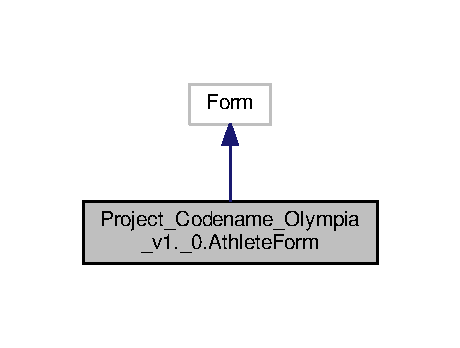
\includegraphics[width=221pt]{classProject__Codename__Olympia__v1_1_1__0_1_1AthleteForm__inherit__graph}
\end{center}
\end{figure}


Collaboration diagram for Project\+\_\+\+Codename\+\_\+\+Olympia\+\_\+v1.\+\_\+0.\+Athlete\+Form\+:
\nopagebreak
\begin{figure}[H]
\begin{center}
\leavevmode
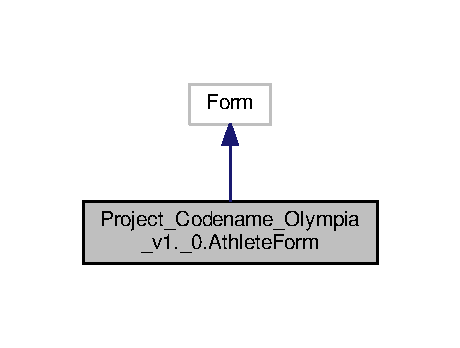
\includegraphics[width=221pt]{classProject__Codename__Olympia__v1_1_1__0_1_1AthleteForm__coll__graph}
\end{center}
\end{figure}
\subsection*{Protected Member Functions}
\begin{DoxyCompactItemize}
\item 
override void \hyperlink{classProject__Codename__Olympia__v1_1_1__0_1_1AthleteForm_a96cf7be874bb0c7f6e0a0a4039cc19eb}{Dispose} (bool disposing)
\begin{DoxyCompactList}\small\item\em Clean up any resources being used. \end{DoxyCompactList}\end{DoxyCompactItemize}


\subsection{Member Function Documentation}
\mbox{\Hypertarget{classProject__Codename__Olympia__v1_1_1__0_1_1AthleteForm_a96cf7be874bb0c7f6e0a0a4039cc19eb}\label{classProject__Codename__Olympia__v1_1_1__0_1_1AthleteForm_a96cf7be874bb0c7f6e0a0a4039cc19eb}} 
\index{Project\+\_\+\+Codename\+\_\+\+Olympia\+\_\+v1\+::\+\_\+0\+::\+Athlete\+Form@{Project\+\_\+\+Codename\+\_\+\+Olympia\+\_\+v1\+::\+\_\+0\+::\+Athlete\+Form}!Dispose@{Dispose}}
\index{Dispose@{Dispose}!Project\+\_\+\+Codename\+\_\+\+Olympia\+\_\+v1\+::\+\_\+0\+::\+Athlete\+Form@{Project\+\_\+\+Codename\+\_\+\+Olympia\+\_\+v1\+::\+\_\+0\+::\+Athlete\+Form}}
\subsubsection{\texorpdfstring{Dispose()}{Dispose()}}
{\footnotesize\ttfamily override void Project\+\_\+\+Codename\+\_\+\+Olympia\+\_\+v1.\+\_\+0.\+Athlete\+Form.\+Dispose (\begin{DoxyParamCaption}\item[{bool}]{disposing }\end{DoxyParamCaption})\hspace{0.3cm}{\ttfamily [inline]}, {\ttfamily [protected]}}



Clean up any resources being used. 


\begin{DoxyParams}{Parameters}
{\em disposing} & true if managed resources should be disposed; otherwise, false.\\
\hline
\end{DoxyParams}


The documentation for this class was generated from the following files\+:\begin{DoxyCompactItemize}
\item 
Form3.\+cs\item 
Form3.\+Designer.\+cs\end{DoxyCompactItemize}

\hypertarget{classProject__Codename__Olympia__v1_1_1__0_1_1Database}{}\section{Project\+\_\+\+Codename\+\_\+\+Olympia\+\_\+v1.\+\_\+0.\+Database Class Reference}
\label{classProject__Codename__Olympia__v1_1_1__0_1_1Database}\index{Project\+\_\+\+Codename\+\_\+\+Olympia\+\_\+v1.\+\_\+0.\+Database@{Project\+\_\+\+Codename\+\_\+\+Olympia\+\_\+v1.\+\_\+0.\+Database}}


Schedule class is the organization of athletes and events.  


\subsection*{Public Member Functions}
\begin{DoxyCompactItemize}
\item 
\hyperlink{classProject__Codename__Olympia__v1_1_1__0_1_1Database_a21b7504aee323670b290e303530b3da7}{Database} ()
\end{DoxyCompactItemize}


\subsection{Detailed Description}
Schedule class is the organization of athletes and events. 

D\+E\+F\+I\+N\+T\+I\+ON\+: The chronological listing of events over the course of two weeks. Scheduling implements where and when events are held. Schedule is also the organization of athletes placed into their respective events.

C\+O\+N\+S\+T\+R\+A\+I\+N\+TS\+: Must not organize events such that they happen concurrently on the same rink. Must not allot more than the appropriate amount of athletes per event. Must make sure any event is done as a pair contains one male and one female athlete per team.\begin{DoxyAuthor}{Author}
Landen Marchand\+D\+E\+P\+R\+E\+C\+A\+T\+E\+D!!! \hyperlink{classProject__Codename__Olympia__v1_1_1__0_1_1Database}{Database} S\+U\+B\+S\+Y\+S\+T\+EM houses all the information of the Winter Olympics
\end{DoxyAuthor}
D\+E\+F\+I\+N\+I\+T\+I\+ON\+: The collection of all information for all events in the Winter Olympics. A database also is a collection of all registrants information.

C\+O\+N\+S\+T\+R\+A\+I\+N\+TS\+: Must contain information apropos to the event and registrants at hand.\begin{DoxyAuthor}{Author}
Landen Marchand 
\end{DoxyAuthor}


\subsection{Constructor \& Destructor Documentation}
\mbox{\Hypertarget{classProject__Codename__Olympia__v1_1_1__0_1_1Database_a21b7504aee323670b290e303530b3da7}\label{classProject__Codename__Olympia__v1_1_1__0_1_1Database_a21b7504aee323670b290e303530b3da7}} 
\index{Project\+\_\+\+Codename\+\_\+\+Olympia\+\_\+v1\+::\+\_\+0\+::\+Database@{Project\+\_\+\+Codename\+\_\+\+Olympia\+\_\+v1\+::\+\_\+0\+::\+Database}!Database@{Database}}
\index{Database@{Database}!Project\+\_\+\+Codename\+\_\+\+Olympia\+\_\+v1\+::\+\_\+0\+::\+Database@{Project\+\_\+\+Codename\+\_\+\+Olympia\+\_\+v1\+::\+\_\+0\+::\+Database}}
\subsubsection{\texorpdfstring{Database()}{Database()}}
{\footnotesize\ttfamily Project\+\_\+\+Codename\+\_\+\+Olympia\+\_\+v1.\+\_\+0.\+Database.\+Database (\begin{DoxyParamCaption}{ }\end{DoxyParamCaption})\hspace{0.3cm}{\ttfamily [inline]}}



The documentation for this class was generated from the following file\+:\begin{DoxyCompactItemize}
\item 
\hyperlink{Class1_8cs}{Class1.\+cs}\end{DoxyCompactItemize}

\hypertarget{classProject__Codename__Olympia__v1_1_1__0_1_1Event}{}\section{Project\+\_\+\+Codename\+\_\+\+Olympia\+\_\+v1.\+\_\+0.\+Event Class Reference}
\label{classProject__Codename__Olympia__v1_1_1__0_1_1Event}\index{Project\+\_\+\+Codename\+\_\+\+Olympia\+\_\+v1.\+\_\+0.\+Event@{Project\+\_\+\+Codename\+\_\+\+Olympia\+\_\+v1.\+\_\+0.\+Event}}


\hyperlink{classProject__Codename__Olympia__v1_1_1__0_1_1Event}{Event} class is the superclass of all the 2 event types and 6 specific events.  


\subsection*{Public Member Functions}
\begin{DoxyCompactItemize}
\item 
\hyperlink{classProject__Codename__Olympia__v1_1_1__0_1_1Event_a1ad8588cb7e2442f64ee90ca32614f85}{Event} ()
\end{DoxyCompactItemize}


\subsection{Detailed Description}
\hyperlink{classProject__Codename__Olympia__v1_1_1__0_1_1Event}{Event} class is the superclass of all the 2 event types and 6 specific events. 

D\+E\+F\+I\+N\+I\+T\+I\+ON\+: The specific competition at a specified rink determined by the schedule.

C\+O\+N\+S\+T\+R\+A\+I\+N\+TS\+: Limited to the six official events of the Winter Olympics. Events will not disturb those who are not registered for that specific event. Expunges the highest and lowest scores an individual or pair receives. Total score is the average of the remaining judges scores. Timed events utilize time as the score which a judge verifies.\begin{DoxyAuthor}{Author}
Landen Marchand 
\end{DoxyAuthor}


\subsection{Constructor \& Destructor Documentation}
\mbox{\Hypertarget{classProject__Codename__Olympia__v1_1_1__0_1_1Event_a1ad8588cb7e2442f64ee90ca32614f85}\label{classProject__Codename__Olympia__v1_1_1__0_1_1Event_a1ad8588cb7e2442f64ee90ca32614f85}} 
\index{Project\+\_\+\+Codename\+\_\+\+Olympia\+\_\+v1\+::\+\_\+0\+::\+Event@{Project\+\_\+\+Codename\+\_\+\+Olympia\+\_\+v1\+::\+\_\+0\+::\+Event}!Event@{Event}}
\index{Event@{Event}!Project\+\_\+\+Codename\+\_\+\+Olympia\+\_\+v1\+::\+\_\+0\+::\+Event@{Project\+\_\+\+Codename\+\_\+\+Olympia\+\_\+v1\+::\+\_\+0\+::\+Event}}
\subsubsection{\texorpdfstring{Event()}{Event()}}
{\footnotesize\ttfamily Project\+\_\+\+Codename\+\_\+\+Olympia\+\_\+v1.\+\_\+0.\+Event.\+Event (\begin{DoxyParamCaption}{ }\end{DoxyParamCaption})\hspace{0.3cm}{\ttfamily [inline]}}

Default Constructor Provided Automatically 
\begin{DoxyParams}{Parameters}
{\em None} & \\
\hline
\end{DoxyParams}
\begin{DoxyReturn}{Returns}
Default Values 
\end{DoxyReturn}


The documentation for this class was generated from the following file\+:\begin{DoxyCompactItemize}
\item 
\hyperlink{Class1_8cs}{Class1.\+cs}\end{DoxyCompactItemize}

\hypertarget{interfaceProject__Codename__Olympia__v1_1_1__0_1_1Event_1_1eventInheritance}{}\section{Project\+\_\+\+Codename\+\_\+\+Olympia\+\_\+v1.\+\_\+0.\+Event.\+event\+Inheritance Interface Reference}
\label{interfaceProject__Codename__Olympia__v1_1_1__0_1_1Event_1_1eventInheritance}\index{Project\+\_\+\+Codename\+\_\+\+Olympia\+\_\+v1.\+\_\+0.\+Event.\+event\+Inheritance@{Project\+\_\+\+Codename\+\_\+\+Olympia\+\_\+v1.\+\_\+0.\+Event.\+event\+Inheritance}}
\subsection*{Public Member Functions}
\begin{DoxyCompactItemize}
\item 
\mbox{\Hypertarget{interfaceProject__Codename__Olympia__v1_1_1__0_1_1Event_1_1eventInheritance_adda2d1d9122f9327f73a0af670551e59}\label{interfaceProject__Codename__Olympia__v1_1_1__0_1_1Event_1_1eventInheritance_adda2d1d9122f9327f73a0af670551e59}} 
int {\bfseries event\+Num} ()
\item 
\mbox{\Hypertarget{interfaceProject__Codename__Olympia__v1_1_1__0_1_1Event_1_1eventInheritance_a89c0953ab749607d5d4e34338e1daac3}\label{interfaceProject__Codename__Olympia__v1_1_1__0_1_1Event_1_1eventInheritance_a89c0953ab749607d5d4e34338e1daac3}} 
void {\bfseries run\+Event} (List$<$ \hyperlink{classProject__Codename__Olympia__v1_1_1__0_1_1Judge}{Judge} $>$ j, List$<$ \hyperlink{classProject__Codename__Olympia__v1_1_1__0_1_1Team}{Team} $>$ t)
\item 
\mbox{\Hypertarget{interfaceProject__Codename__Olympia__v1_1_1__0_1_1Event_1_1eventInheritance_a440deb71af87d95041fb3a64e869de39}\label{interfaceProject__Codename__Olympia__v1_1_1__0_1_1Event_1_1eventInheritance_a440deb71af87d95041fb3a64e869de39}} 
void {\bfseries sched\+Event} (List$<$ \hyperlink{classProject__Codename__Olympia__v1_1_1__0_1_1Judge}{Judge} $>$ j, List$<$ \hyperlink{classProject__Codename__Olympia__v1_1_1__0_1_1Team}{Team} $>$ t)
\end{DoxyCompactItemize}


\subsection{Detailed Description}
Inheritance member function for \hyperlink{classProject__Codename__Olympia__v1_1_1__0_1_1SpeedSkating}{Speed\+Skating} and \hyperlink{classProject__Codename__Olympia__v1_1_1__0_1_1FigureSkating}{Figure\+Skating} events /$\ast$$\ast$ Interface so \hyperlink{classProject__Codename__Olympia__v1_1_1__0_1_1SpeedSkating}{Speed\+Skating} and \hyperlink{classProject__Codename__Olympia__v1_1_1__0_1_1FigureSkating}{Figure\+Skating} events can utilize inherited functions 

The documentation for this interface was generated from the following file\+:\begin{DoxyCompactItemize}
\item 
Class1.\+cs\end{DoxyCompactItemize}

\hypertarget{classProject__Codename__Olympia__v1_1_1__0_1_1FigureSkating}{}\section{Project\+\_\+\+Codename\+\_\+\+Olympia\+\_\+v1.\+\_\+0.\+Figure\+Skating Class Reference}
\label{classProject__Codename__Olympia__v1_1_1__0_1_1FigureSkating}\index{Project\+\_\+\+Codename\+\_\+\+Olympia\+\_\+v1.\+\_\+0.\+Figure\+Skating@{Project\+\_\+\+Codename\+\_\+\+Olympia\+\_\+v1.\+\_\+0.\+Figure\+Skating}}


\hyperlink{classProject__Codename__Olympia__v1_1_1__0_1_1FigureSkating}{Figure\+Skating} class is the superclass of the 3 \hyperlink{classProject__Codename__Olympia__v1_1_1__0_1_1FigureSkating}{Figure\+Skating} events.  




Inheritance diagram for Project\+\_\+\+Codename\+\_\+\+Olympia\+\_\+v1.\+\_\+0.\+Figure\+Skating\+:
\nopagebreak
\begin{figure}[H]
\begin{center}
\leavevmode
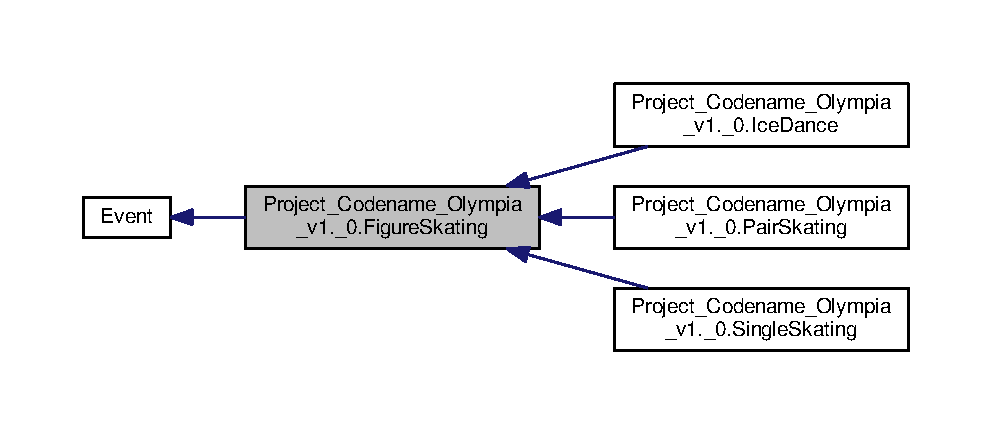
\includegraphics[width=350pt]{classProject__Codename__Olympia__v1_1_1__0_1_1FigureSkating__inherit__graph}
\end{center}
\end{figure}


Collaboration diagram for Project\+\_\+\+Codename\+\_\+\+Olympia\+\_\+v1.\+\_\+0.\+Figure\+Skating\+:
\nopagebreak
\begin{figure}[H]
\begin{center}
\leavevmode
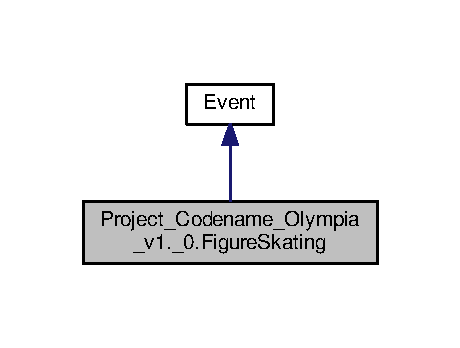
\includegraphics[width=221pt]{classProject__Codename__Olympia__v1_1_1__0_1_1FigureSkating__coll__graph}
\end{center}
\end{figure}
\subsection*{Classes}
\begin{DoxyCompactItemize}
\item 
interface \hyperlink{interfaceProject__Codename__Olympia__v1_1_1__0_1_1FigureSkating_1_1ssInheritance}{ss\+Inheritance}
\end{DoxyCompactItemize}
\subsection*{Public Member Functions}
\begin{DoxyCompactItemize}
\item 
\hyperlink{classProject__Codename__Olympia__v1_1_1__0_1_1FigureSkating_a8b84d8dab64fc0add779a2579c3df1b0}{Figure\+Skating} ()
\item 
abstract double \hyperlink{classProject__Codename__Olympia__v1_1_1__0_1_1FigureSkating_a437e794fec382863421f8c65e31295f8}{fs\+Score} ()
\end{DoxyCompactItemize}


\subsection{Detailed Description}
\hyperlink{classProject__Codename__Olympia__v1_1_1__0_1_1FigureSkating}{Figure\+Skating} class is the superclass of the 3 \hyperlink{classProject__Codename__Olympia__v1_1_1__0_1_1FigureSkating}{Figure\+Skating} events. 

D\+E\+F\+I\+N\+I\+T\+I\+ON\+: Skating done on ice in synchronization with music that is scored based upon technical tricks and or the synchronization of each athlete in a pair. One of the two main sporting categories that consist of three unique events which athletes participate separately as well as in pairs.

C\+O\+N\+S\+T\+R\+A\+I\+N\+TS\+: None\begin{DoxyAuthor}{Author}
Landen Marchand 
\end{DoxyAuthor}


\subsection{Constructor \& Destructor Documentation}
\mbox{\Hypertarget{classProject__Codename__Olympia__v1_1_1__0_1_1FigureSkating_a8b84d8dab64fc0add779a2579c3df1b0}\label{classProject__Codename__Olympia__v1_1_1__0_1_1FigureSkating_a8b84d8dab64fc0add779a2579c3df1b0}} 
\index{Project\+\_\+\+Codename\+\_\+\+Olympia\+\_\+v1\+::\+\_\+0\+::\+Figure\+Skating@{Project\+\_\+\+Codename\+\_\+\+Olympia\+\_\+v1\+::\+\_\+0\+::\+Figure\+Skating}!Figure\+Skating@{Figure\+Skating}}
\index{Figure\+Skating@{Figure\+Skating}!Project\+\_\+\+Codename\+\_\+\+Olympia\+\_\+v1\+::\+\_\+0\+::\+Figure\+Skating@{Project\+\_\+\+Codename\+\_\+\+Olympia\+\_\+v1\+::\+\_\+0\+::\+Figure\+Skating}}
\subsubsection{\texorpdfstring{Figure\+Skating()}{FigureSkating()}}
{\footnotesize\ttfamily Project\+\_\+\+Codename\+\_\+\+Olympia\+\_\+v1.\+\_\+0.\+Figure\+Skating.\+Figure\+Skating (\begin{DoxyParamCaption}{ }\end{DoxyParamCaption})\hspace{0.3cm}{\ttfamily [inline]}}

Default Constructor Provided Automatically 
\begin{DoxyParams}{Parameters}
{\em None} & \\
\hline
\end{DoxyParams}
\begin{DoxyReturn}{Returns}
Default Values 
\end{DoxyReturn}


\subsection{Member Function Documentation}
\mbox{\Hypertarget{classProject__Codename__Olympia__v1_1_1__0_1_1FigureSkating_a437e794fec382863421f8c65e31295f8}\label{classProject__Codename__Olympia__v1_1_1__0_1_1FigureSkating_a437e794fec382863421f8c65e31295f8}} 
\index{Project\+\_\+\+Codename\+\_\+\+Olympia\+\_\+v1\+::\+\_\+0\+::\+Figure\+Skating@{Project\+\_\+\+Codename\+\_\+\+Olympia\+\_\+v1\+::\+\_\+0\+::\+Figure\+Skating}!fs\+Score@{fs\+Score}}
\index{fs\+Score@{fs\+Score}!Project\+\_\+\+Codename\+\_\+\+Olympia\+\_\+v1\+::\+\_\+0\+::\+Figure\+Skating@{Project\+\_\+\+Codename\+\_\+\+Olympia\+\_\+v1\+::\+\_\+0\+::\+Figure\+Skating}}
\subsubsection{\texorpdfstring{fs\+Score()}{fsScore()}}
{\footnotesize\ttfamily abstract double Project\+\_\+\+Codename\+\_\+\+Olympia\+\_\+v1.\+\_\+0.\+Figure\+Skating.\+fs\+Score (\begin{DoxyParamCaption}{ }\end{DoxyParamCaption})\hspace{0.3cm}{\ttfamily [pure virtual]}}

Inheritance member function for \hyperlink{classProject__Codename__Olympia__v1_1_1__0_1_1FigureSkating}{Figure\+Skating} events 
\begin{DoxyParams}{Parameters}
{\em none} & \\
\hline
\end{DoxyParams}
\begin{DoxyReturn}{Returns}
double pertaining to scores (completion of event of athlete) 
\end{DoxyReturn}


Implemented in \hyperlink{classProject__Codename__Olympia__v1_1_1__0_1_1SingleSkating_a0f1837cfe29187ca1c2402f6312f2465}{Project\+\_\+\+Codename\+\_\+\+Olympia\+\_\+v1.\+\_\+0.\+Single\+Skating}, \hyperlink{classProject__Codename__Olympia__v1_1_1__0_1_1PairSkating_aef6f7313446386c4e6bdf8a438e246a1}{Project\+\_\+\+Codename\+\_\+\+Olympia\+\_\+v1.\+\_\+0.\+Pair\+Skating}, and \hyperlink{classProject__Codename__Olympia__v1_1_1__0_1_1IceDance_ad7e7867e61839151b62fd0bbafc09fad}{Project\+\_\+\+Codename\+\_\+\+Olympia\+\_\+v1.\+\_\+0.\+Ice\+Dance}.



The documentation for this class was generated from the following file\+:\begin{DoxyCompactItemize}
\item 
Class1.\+cs\end{DoxyCompactItemize}

\hypertarget{classProject__Codename__Olympia__v1_1_1__0_1_1Form1}{}\section{Project\+\_\+\+Codename\+\_\+\+Olympia\+\_\+v1.\+\_\+0.\+Form1 Class Reference}
\label{classProject__Codename__Olympia__v1_1_1__0_1_1Form1}\index{Project\+\_\+\+Codename\+\_\+\+Olympia\+\_\+v1.\+\_\+0.\+Form1@{Project\+\_\+\+Codename\+\_\+\+Olympia\+\_\+v1.\+\_\+0.\+Form1}}


Inheritance diagram for Project\+\_\+\+Codename\+\_\+\+Olympia\+\_\+v1.\+\_\+0.\+Form1\+:\nopagebreak
\begin{figure}[H]
\begin{center}
\leavevmode
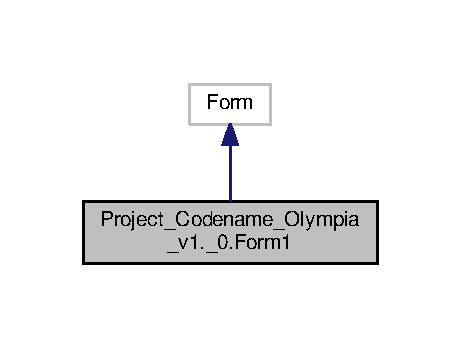
\includegraphics[width=241pt]{classProject__Codename__Olympia__v1_1_1__0_1_1Form1__inherit__graph}
\end{center}
\end{figure}


Collaboration diagram for Project\+\_\+\+Codename\+\_\+\+Olympia\+\_\+v1.\+\_\+0.\+Form1\+:\nopagebreak
\begin{figure}[H]
\begin{center}
\leavevmode
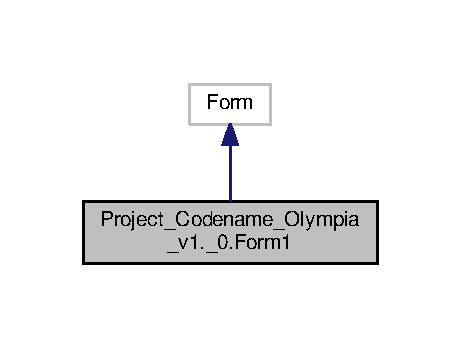
\includegraphics[width=249pt]{classProject__Codename__Olympia__v1_1_1__0_1_1Form1__coll__graph}
\end{center}
\end{figure}
\subsection*{Public Member Functions}
\begin{DoxyCompactItemize}
\item 
\hyperlink{classProject__Codename__Olympia__v1_1_1__0_1_1Form1_acb6249f34e074a6f5edbc137df25bc4c}{Form1} ()
\end{DoxyCompactItemize}
\subsection*{Protected Member Functions}
\begin{DoxyCompactItemize}
\item 
override void \hyperlink{classProject__Codename__Olympia__v1_1_1__0_1_1Form1_aaa9416dc0391b442a1b3d54968a89123}{Dispose} (bool disposing)
\begin{DoxyCompactList}\small\item\em Clean up any resources being used. \end{DoxyCompactList}\end{DoxyCompactItemize}
\subsection*{Private Member Functions}
\begin{DoxyCompactItemize}
\item 
void \hyperlink{classProject__Codename__Olympia__v1_1_1__0_1_1Form1_aa3c3d74fba87a109ffba8cf0100dd0fd}{Form1\+\_\+\+Load} (object sender, Event\+Args e)
\item 
void \hyperlink{classProject__Codename__Olympia__v1_1_1__0_1_1Form1_a4ad71033ec8c4dfd985e859f26d8a506}{button1\+\_\+\+Click} (object sender, Event\+Args e)
\item 
void \hyperlink{classProject__Codename__Olympia__v1_1_1__0_1_1Form1_ad8c23cc40fa8242ec003291e553d2d50}{button2\+\_\+\+Click} (object sender, Event\+Args e)
\item 
void \hyperlink{classProject__Codename__Olympia__v1_1_1__0_1_1Form1_a76210a69592d0b1adc336d9837a32afa}{button5\+\_\+\+Click} (object sender, Event\+Args e)
\item 
void \hyperlink{classProject__Codename__Olympia__v1_1_1__0_1_1Form1_a53663e1408c2ef4ab861d5022be2ed14}{button3\+\_\+\+Click} (object sender, Event\+Args e)
\item 
void \hyperlink{classProject__Codename__Olympia__v1_1_1__0_1_1Form1_a464a4a8e8798de8a1f12242da6b917b7}{button4\+\_\+\+Click} (object sender, Event\+Args e)
\item 
void \hyperlink{classProject__Codename__Olympia__v1_1_1__0_1_1Form1_a63f3e34c4506e1339de2ce5880414cd8}{Initialize\+Component} ()
\begin{DoxyCompactList}\small\item\em Required method for Designer support -\/ do not modify the contents of this method with the code editor. \end{DoxyCompactList}\end{DoxyCompactItemize}
\subsection*{Private Attributes}
\begin{DoxyCompactItemize}
\item 
System.\+Component\+Model.\+I\+Container \hyperlink{classProject__Codename__Olympia__v1_1_1__0_1_1Form1_afc1f1595dbcf8ab191592c6930301a0f}{components} = null
\begin{DoxyCompactList}\small\item\em Required designer variable. \end{DoxyCompactList}\item 
System.\+Windows.\+Forms.\+Button \hyperlink{classProject__Codename__Olympia__v1_1_1__0_1_1Form1_a5656361ec4351d173db39628515c9a5a}{button1}
\item 
System.\+Windows.\+Forms.\+Button \hyperlink{classProject__Codename__Olympia__v1_1_1__0_1_1Form1_a642b0136b529a2ce0b193657ea742059}{button2}
\item 
System.\+Windows.\+Forms.\+Button \hyperlink{classProject__Codename__Olympia__v1_1_1__0_1_1Form1_afc577c228081df6efa01a0dc28e5f209}{button3}
\item 
System.\+Windows.\+Forms.\+Button \hyperlink{classProject__Codename__Olympia__v1_1_1__0_1_1Form1_ac04935f86732650f5f64798f289e2017}{button4}
\item 
System.\+Windows.\+Forms.\+Label \hyperlink{classProject__Codename__Olympia__v1_1_1__0_1_1Form1_a37bc2a4e841f3a2b5ca4ff064f0d2a9c}{label1}
\item 
System.\+Windows.\+Forms.\+Label \hyperlink{classProject__Codename__Olympia__v1_1_1__0_1_1Form1_a8f282aae1178b3cc1b18ee8f37115b53}{label2}
\item 
System.\+Windows.\+Forms.\+Label \hyperlink{classProject__Codename__Olympia__v1_1_1__0_1_1Form1_a79cfe899ae6a084d7fe28674e7fab51c}{label3}
\item 
System.\+Windows.\+Forms.\+Label \hyperlink{classProject__Codename__Olympia__v1_1_1__0_1_1Form1_a948d2092c62f8251d48232e6c1fe1813}{label4}
\item 
System.\+Windows.\+Forms.\+Label \hyperlink{classProject__Codename__Olympia__v1_1_1__0_1_1Form1_adac4bdce2b9b0118cb9344967ce6d851}{label5}
\item 
System.\+Windows.\+Forms.\+Button \hyperlink{classProject__Codename__Olympia__v1_1_1__0_1_1Form1_a0af2249b8906aca5a318040729e95fc0}{button5}
\end{DoxyCompactItemize}


\subsection{Detailed Description}


Definition at line 17 of file Form1.\+cs.



\subsection{Constructor \& Destructor Documentation}
\mbox{\Hypertarget{classProject__Codename__Olympia__v1_1_1__0_1_1Form1_acb6249f34e074a6f5edbc137df25bc4c}\label{classProject__Codename__Olympia__v1_1_1__0_1_1Form1_acb6249f34e074a6f5edbc137df25bc4c}} 
\index{Project\+\_\+\+Codename\+\_\+\+Olympia\+\_\+v1\+::\+\_\+0\+::\+Form1@{Project\+\_\+\+Codename\+\_\+\+Olympia\+\_\+v1\+::\+\_\+0\+::\+Form1}!Form1@{Form1}}
\index{Form1@{Form1}!Project\+\_\+\+Codename\+\_\+\+Olympia\+\_\+v1\+::\+\_\+0\+::\+Form1@{Project\+\_\+\+Codename\+\_\+\+Olympia\+\_\+v1\+::\+\_\+0\+::\+Form1}}
\subsubsection{\texorpdfstring{Form1()}{Form1()}}
{\footnotesize\ttfamily Project\+\_\+\+Codename\+\_\+\+Olympia\+\_\+v1.\+\_\+0.\+Form1.\+Form1 (\begin{DoxyParamCaption}{ }\end{DoxyParamCaption})\hspace{0.3cm}{\ttfamily [inline]}}



Definition at line 20 of file Form1.\+cs.



\subsection{Member Function Documentation}
\mbox{\Hypertarget{classProject__Codename__Olympia__v1_1_1__0_1_1Form1_a4ad71033ec8c4dfd985e859f26d8a506}\label{classProject__Codename__Olympia__v1_1_1__0_1_1Form1_a4ad71033ec8c4dfd985e859f26d8a506}} 
\index{Project\+\_\+\+Codename\+\_\+\+Olympia\+\_\+v1\+::\+\_\+0\+::\+Form1@{Project\+\_\+\+Codename\+\_\+\+Olympia\+\_\+v1\+::\+\_\+0\+::\+Form1}!button1\+\_\+\+Click@{button1\+\_\+\+Click}}
\index{button1\+\_\+\+Click@{button1\+\_\+\+Click}!Project\+\_\+\+Codename\+\_\+\+Olympia\+\_\+v1\+::\+\_\+0\+::\+Form1@{Project\+\_\+\+Codename\+\_\+\+Olympia\+\_\+v1\+::\+\_\+0\+::\+Form1}}
\subsubsection{\texorpdfstring{button1\+\_\+\+Click()}{button1\_Click()}}
{\footnotesize\ttfamily void Project\+\_\+\+Codename\+\_\+\+Olympia\+\_\+v1.\+\_\+0.\+Form1.\+button1\+\_\+\+Click (\begin{DoxyParamCaption}\item[{object}]{sender,  }\item[{Event\+Args}]{e }\end{DoxyParamCaption})\hspace{0.3cm}{\ttfamily [inline]}, {\ttfamily [private]}}



Definition at line 30 of file Form1.\+cs.

\mbox{\Hypertarget{classProject__Codename__Olympia__v1_1_1__0_1_1Form1_ad8c23cc40fa8242ec003291e553d2d50}\label{classProject__Codename__Olympia__v1_1_1__0_1_1Form1_ad8c23cc40fa8242ec003291e553d2d50}} 
\index{Project\+\_\+\+Codename\+\_\+\+Olympia\+\_\+v1\+::\+\_\+0\+::\+Form1@{Project\+\_\+\+Codename\+\_\+\+Olympia\+\_\+v1\+::\+\_\+0\+::\+Form1}!button2\+\_\+\+Click@{button2\+\_\+\+Click}}
\index{button2\+\_\+\+Click@{button2\+\_\+\+Click}!Project\+\_\+\+Codename\+\_\+\+Olympia\+\_\+v1\+::\+\_\+0\+::\+Form1@{Project\+\_\+\+Codename\+\_\+\+Olympia\+\_\+v1\+::\+\_\+0\+::\+Form1}}
\subsubsection{\texorpdfstring{button2\+\_\+\+Click()}{button2\_Click()}}
{\footnotesize\ttfamily void Project\+\_\+\+Codename\+\_\+\+Olympia\+\_\+v1.\+\_\+0.\+Form1.\+button2\+\_\+\+Click (\begin{DoxyParamCaption}\item[{object}]{sender,  }\item[{Event\+Args}]{e }\end{DoxyParamCaption})\hspace{0.3cm}{\ttfamily [inline]}, {\ttfamily [private]}}



Definition at line 36 of file Form1.\+cs.

\mbox{\Hypertarget{classProject__Codename__Olympia__v1_1_1__0_1_1Form1_a53663e1408c2ef4ab861d5022be2ed14}\label{classProject__Codename__Olympia__v1_1_1__0_1_1Form1_a53663e1408c2ef4ab861d5022be2ed14}} 
\index{Project\+\_\+\+Codename\+\_\+\+Olympia\+\_\+v1\+::\+\_\+0\+::\+Form1@{Project\+\_\+\+Codename\+\_\+\+Olympia\+\_\+v1\+::\+\_\+0\+::\+Form1}!button3\+\_\+\+Click@{button3\+\_\+\+Click}}
\index{button3\+\_\+\+Click@{button3\+\_\+\+Click}!Project\+\_\+\+Codename\+\_\+\+Olympia\+\_\+v1\+::\+\_\+0\+::\+Form1@{Project\+\_\+\+Codename\+\_\+\+Olympia\+\_\+v1\+::\+\_\+0\+::\+Form1}}
\subsubsection{\texorpdfstring{button3\+\_\+\+Click()}{button3\_Click()}}
{\footnotesize\ttfamily void Project\+\_\+\+Codename\+\_\+\+Olympia\+\_\+v1.\+\_\+0.\+Form1.\+button3\+\_\+\+Click (\begin{DoxyParamCaption}\item[{object}]{sender,  }\item[{Event\+Args}]{e }\end{DoxyParamCaption})\hspace{0.3cm}{\ttfamily [inline]}, {\ttfamily [private]}}



Definition at line 48 of file Form1.\+cs.

\mbox{\Hypertarget{classProject__Codename__Olympia__v1_1_1__0_1_1Form1_a464a4a8e8798de8a1f12242da6b917b7}\label{classProject__Codename__Olympia__v1_1_1__0_1_1Form1_a464a4a8e8798de8a1f12242da6b917b7}} 
\index{Project\+\_\+\+Codename\+\_\+\+Olympia\+\_\+v1\+::\+\_\+0\+::\+Form1@{Project\+\_\+\+Codename\+\_\+\+Olympia\+\_\+v1\+::\+\_\+0\+::\+Form1}!button4\+\_\+\+Click@{button4\+\_\+\+Click}}
\index{button4\+\_\+\+Click@{button4\+\_\+\+Click}!Project\+\_\+\+Codename\+\_\+\+Olympia\+\_\+v1\+::\+\_\+0\+::\+Form1@{Project\+\_\+\+Codename\+\_\+\+Olympia\+\_\+v1\+::\+\_\+0\+::\+Form1}}
\subsubsection{\texorpdfstring{button4\+\_\+\+Click()}{button4\_Click()}}
{\footnotesize\ttfamily void Project\+\_\+\+Codename\+\_\+\+Olympia\+\_\+v1.\+\_\+0.\+Form1.\+button4\+\_\+\+Click (\begin{DoxyParamCaption}\item[{object}]{sender,  }\item[{Event\+Args}]{e }\end{DoxyParamCaption})\hspace{0.3cm}{\ttfamily [inline]}, {\ttfamily [private]}}



Definition at line 54 of file Form1.\+cs.

\mbox{\Hypertarget{classProject__Codename__Olympia__v1_1_1__0_1_1Form1_a76210a69592d0b1adc336d9837a32afa}\label{classProject__Codename__Olympia__v1_1_1__0_1_1Form1_a76210a69592d0b1adc336d9837a32afa}} 
\index{Project\+\_\+\+Codename\+\_\+\+Olympia\+\_\+v1\+::\+\_\+0\+::\+Form1@{Project\+\_\+\+Codename\+\_\+\+Olympia\+\_\+v1\+::\+\_\+0\+::\+Form1}!button5\+\_\+\+Click@{button5\+\_\+\+Click}}
\index{button5\+\_\+\+Click@{button5\+\_\+\+Click}!Project\+\_\+\+Codename\+\_\+\+Olympia\+\_\+v1\+::\+\_\+0\+::\+Form1@{Project\+\_\+\+Codename\+\_\+\+Olympia\+\_\+v1\+::\+\_\+0\+::\+Form1}}
\subsubsection{\texorpdfstring{button5\+\_\+\+Click()}{button5\_Click()}}
{\footnotesize\ttfamily void Project\+\_\+\+Codename\+\_\+\+Olympia\+\_\+v1.\+\_\+0.\+Form1.\+button5\+\_\+\+Click (\begin{DoxyParamCaption}\item[{object}]{sender,  }\item[{Event\+Args}]{e }\end{DoxyParamCaption})\hspace{0.3cm}{\ttfamily [inline]}, {\ttfamily [private]}}



Definition at line 42 of file Form1.\+cs.

\mbox{\Hypertarget{classProject__Codename__Olympia__v1_1_1__0_1_1Form1_aaa9416dc0391b442a1b3d54968a89123}\label{classProject__Codename__Olympia__v1_1_1__0_1_1Form1_aaa9416dc0391b442a1b3d54968a89123}} 
\index{Project\+\_\+\+Codename\+\_\+\+Olympia\+\_\+v1\+::\+\_\+0\+::\+Form1@{Project\+\_\+\+Codename\+\_\+\+Olympia\+\_\+v1\+::\+\_\+0\+::\+Form1}!Dispose@{Dispose}}
\index{Dispose@{Dispose}!Project\+\_\+\+Codename\+\_\+\+Olympia\+\_\+v1\+::\+\_\+0\+::\+Form1@{Project\+\_\+\+Codename\+\_\+\+Olympia\+\_\+v1\+::\+\_\+0\+::\+Form1}}
\subsubsection{\texorpdfstring{Dispose()}{Dispose()}}
{\footnotesize\ttfamily override void Project\+\_\+\+Codename\+\_\+\+Olympia\+\_\+v1.\+\_\+0.\+Form1.\+Dispose (\begin{DoxyParamCaption}\item[{bool}]{disposing }\end{DoxyParamCaption})\hspace{0.3cm}{\ttfamily [inline]}, {\ttfamily [protected]}}



Clean up any resources being used. 


\begin{DoxyParams}{Parameters}
{\em disposing} & true if managed resources should be disposed; otherwise, false.\\
\hline
\end{DoxyParams}


Definition at line 14 of file Form1.\+Designer.\+cs.

\mbox{\Hypertarget{classProject__Codename__Olympia__v1_1_1__0_1_1Form1_aa3c3d74fba87a109ffba8cf0100dd0fd}\label{classProject__Codename__Olympia__v1_1_1__0_1_1Form1_aa3c3d74fba87a109ffba8cf0100dd0fd}} 
\index{Project\+\_\+\+Codename\+\_\+\+Olympia\+\_\+v1\+::\+\_\+0\+::\+Form1@{Project\+\_\+\+Codename\+\_\+\+Olympia\+\_\+v1\+::\+\_\+0\+::\+Form1}!Form1\+\_\+\+Load@{Form1\+\_\+\+Load}}
\index{Form1\+\_\+\+Load@{Form1\+\_\+\+Load}!Project\+\_\+\+Codename\+\_\+\+Olympia\+\_\+v1\+::\+\_\+0\+::\+Form1@{Project\+\_\+\+Codename\+\_\+\+Olympia\+\_\+v1\+::\+\_\+0\+::\+Form1}}
\subsubsection{\texorpdfstring{Form1\+\_\+\+Load()}{Form1\_Load()}}
{\footnotesize\ttfamily void Project\+\_\+\+Codename\+\_\+\+Olympia\+\_\+v1.\+\_\+0.\+Form1.\+Form1\+\_\+\+Load (\begin{DoxyParamCaption}\item[{object}]{sender,  }\item[{Event\+Args}]{e }\end{DoxyParamCaption})\hspace{0.3cm}{\ttfamily [inline]}, {\ttfamily [private]}}



Definition at line 25 of file Form1.\+cs.

\mbox{\Hypertarget{classProject__Codename__Olympia__v1_1_1__0_1_1Form1_a63f3e34c4506e1339de2ce5880414cd8}\label{classProject__Codename__Olympia__v1_1_1__0_1_1Form1_a63f3e34c4506e1339de2ce5880414cd8}} 
\index{Project\+\_\+\+Codename\+\_\+\+Olympia\+\_\+v1\+::\+\_\+0\+::\+Form1@{Project\+\_\+\+Codename\+\_\+\+Olympia\+\_\+v1\+::\+\_\+0\+::\+Form1}!Initialize\+Component@{Initialize\+Component}}
\index{Initialize\+Component@{Initialize\+Component}!Project\+\_\+\+Codename\+\_\+\+Olympia\+\_\+v1\+::\+\_\+0\+::\+Form1@{Project\+\_\+\+Codename\+\_\+\+Olympia\+\_\+v1\+::\+\_\+0\+::\+Form1}}
\subsubsection{\texorpdfstring{Initialize\+Component()}{InitializeComponent()}}
{\footnotesize\ttfamily void Project\+\_\+\+Codename\+\_\+\+Olympia\+\_\+v1.\+\_\+0.\+Form1.\+Initialize\+Component (\begin{DoxyParamCaption}{ }\end{DoxyParamCaption})\hspace{0.3cm}{\ttfamily [inline]}, {\ttfamily [private]}}



Required method for Designer support -\/ do not modify the contents of this method with the code editor. 



Definition at line 29 of file Form1.\+Designer.\+cs.



\subsection{Member Data Documentation}
\mbox{\Hypertarget{classProject__Codename__Olympia__v1_1_1__0_1_1Form1_a5656361ec4351d173db39628515c9a5a}\label{classProject__Codename__Olympia__v1_1_1__0_1_1Form1_a5656361ec4351d173db39628515c9a5a}} 
\index{Project\+\_\+\+Codename\+\_\+\+Olympia\+\_\+v1\+::\+\_\+0\+::\+Form1@{Project\+\_\+\+Codename\+\_\+\+Olympia\+\_\+v1\+::\+\_\+0\+::\+Form1}!button1@{button1}}
\index{button1@{button1}!Project\+\_\+\+Codename\+\_\+\+Olympia\+\_\+v1\+::\+\_\+0\+::\+Form1@{Project\+\_\+\+Codename\+\_\+\+Olympia\+\_\+v1\+::\+\_\+0\+::\+Form1}}
\subsubsection{\texorpdfstring{button1}{button1}}
{\footnotesize\ttfamily System.\+Windows.\+Forms.\+Button Project\+\_\+\+Codename\+\_\+\+Olympia\+\_\+v1.\+\_\+0.\+Form1.\+button1\hspace{0.3cm}{\ttfamily [private]}}



Definition at line 165 of file Form1.\+Designer.\+cs.

\mbox{\Hypertarget{classProject__Codename__Olympia__v1_1_1__0_1_1Form1_a642b0136b529a2ce0b193657ea742059}\label{classProject__Codename__Olympia__v1_1_1__0_1_1Form1_a642b0136b529a2ce0b193657ea742059}} 
\index{Project\+\_\+\+Codename\+\_\+\+Olympia\+\_\+v1\+::\+\_\+0\+::\+Form1@{Project\+\_\+\+Codename\+\_\+\+Olympia\+\_\+v1\+::\+\_\+0\+::\+Form1}!button2@{button2}}
\index{button2@{button2}!Project\+\_\+\+Codename\+\_\+\+Olympia\+\_\+v1\+::\+\_\+0\+::\+Form1@{Project\+\_\+\+Codename\+\_\+\+Olympia\+\_\+v1\+::\+\_\+0\+::\+Form1}}
\subsubsection{\texorpdfstring{button2}{button2}}
{\footnotesize\ttfamily System.\+Windows.\+Forms.\+Button Project\+\_\+\+Codename\+\_\+\+Olympia\+\_\+v1.\+\_\+0.\+Form1.\+button2\hspace{0.3cm}{\ttfamily [private]}}



Definition at line 166 of file Form1.\+Designer.\+cs.

\mbox{\Hypertarget{classProject__Codename__Olympia__v1_1_1__0_1_1Form1_afc577c228081df6efa01a0dc28e5f209}\label{classProject__Codename__Olympia__v1_1_1__0_1_1Form1_afc577c228081df6efa01a0dc28e5f209}} 
\index{Project\+\_\+\+Codename\+\_\+\+Olympia\+\_\+v1\+::\+\_\+0\+::\+Form1@{Project\+\_\+\+Codename\+\_\+\+Olympia\+\_\+v1\+::\+\_\+0\+::\+Form1}!button3@{button3}}
\index{button3@{button3}!Project\+\_\+\+Codename\+\_\+\+Olympia\+\_\+v1\+::\+\_\+0\+::\+Form1@{Project\+\_\+\+Codename\+\_\+\+Olympia\+\_\+v1\+::\+\_\+0\+::\+Form1}}
\subsubsection{\texorpdfstring{button3}{button3}}
{\footnotesize\ttfamily System.\+Windows.\+Forms.\+Button Project\+\_\+\+Codename\+\_\+\+Olympia\+\_\+v1.\+\_\+0.\+Form1.\+button3\hspace{0.3cm}{\ttfamily [private]}}



Definition at line 167 of file Form1.\+Designer.\+cs.

\mbox{\Hypertarget{classProject__Codename__Olympia__v1_1_1__0_1_1Form1_ac04935f86732650f5f64798f289e2017}\label{classProject__Codename__Olympia__v1_1_1__0_1_1Form1_ac04935f86732650f5f64798f289e2017}} 
\index{Project\+\_\+\+Codename\+\_\+\+Olympia\+\_\+v1\+::\+\_\+0\+::\+Form1@{Project\+\_\+\+Codename\+\_\+\+Olympia\+\_\+v1\+::\+\_\+0\+::\+Form1}!button4@{button4}}
\index{button4@{button4}!Project\+\_\+\+Codename\+\_\+\+Olympia\+\_\+v1\+::\+\_\+0\+::\+Form1@{Project\+\_\+\+Codename\+\_\+\+Olympia\+\_\+v1\+::\+\_\+0\+::\+Form1}}
\subsubsection{\texorpdfstring{button4}{button4}}
{\footnotesize\ttfamily System.\+Windows.\+Forms.\+Button Project\+\_\+\+Codename\+\_\+\+Olympia\+\_\+v1.\+\_\+0.\+Form1.\+button4\hspace{0.3cm}{\ttfamily [private]}}



Definition at line 168 of file Form1.\+Designer.\+cs.

\mbox{\Hypertarget{classProject__Codename__Olympia__v1_1_1__0_1_1Form1_a0af2249b8906aca5a318040729e95fc0}\label{classProject__Codename__Olympia__v1_1_1__0_1_1Form1_a0af2249b8906aca5a318040729e95fc0}} 
\index{Project\+\_\+\+Codename\+\_\+\+Olympia\+\_\+v1\+::\+\_\+0\+::\+Form1@{Project\+\_\+\+Codename\+\_\+\+Olympia\+\_\+v1\+::\+\_\+0\+::\+Form1}!button5@{button5}}
\index{button5@{button5}!Project\+\_\+\+Codename\+\_\+\+Olympia\+\_\+v1\+::\+\_\+0\+::\+Form1@{Project\+\_\+\+Codename\+\_\+\+Olympia\+\_\+v1\+::\+\_\+0\+::\+Form1}}
\subsubsection{\texorpdfstring{button5}{button5}}
{\footnotesize\ttfamily System.\+Windows.\+Forms.\+Button Project\+\_\+\+Codename\+\_\+\+Olympia\+\_\+v1.\+\_\+0.\+Form1.\+button5\hspace{0.3cm}{\ttfamily [private]}}



Definition at line 174 of file Form1.\+Designer.\+cs.

\mbox{\Hypertarget{classProject__Codename__Olympia__v1_1_1__0_1_1Form1_afc1f1595dbcf8ab191592c6930301a0f}\label{classProject__Codename__Olympia__v1_1_1__0_1_1Form1_afc1f1595dbcf8ab191592c6930301a0f}} 
\index{Project\+\_\+\+Codename\+\_\+\+Olympia\+\_\+v1\+::\+\_\+0\+::\+Form1@{Project\+\_\+\+Codename\+\_\+\+Olympia\+\_\+v1\+::\+\_\+0\+::\+Form1}!components@{components}}
\index{components@{components}!Project\+\_\+\+Codename\+\_\+\+Olympia\+\_\+v1\+::\+\_\+0\+::\+Form1@{Project\+\_\+\+Codename\+\_\+\+Olympia\+\_\+v1\+::\+\_\+0\+::\+Form1}}
\subsubsection{\texorpdfstring{components}{components}}
{\footnotesize\ttfamily System.\+Component\+Model.\+I\+Container Project\+\_\+\+Codename\+\_\+\+Olympia\+\_\+v1.\+\_\+0.\+Form1.\+components = null\hspace{0.3cm}{\ttfamily [private]}}



Required designer variable. 



Definition at line 8 of file Form1.\+Designer.\+cs.

\mbox{\Hypertarget{classProject__Codename__Olympia__v1_1_1__0_1_1Form1_a37bc2a4e841f3a2b5ca4ff064f0d2a9c}\label{classProject__Codename__Olympia__v1_1_1__0_1_1Form1_a37bc2a4e841f3a2b5ca4ff064f0d2a9c}} 
\index{Project\+\_\+\+Codename\+\_\+\+Olympia\+\_\+v1\+::\+\_\+0\+::\+Form1@{Project\+\_\+\+Codename\+\_\+\+Olympia\+\_\+v1\+::\+\_\+0\+::\+Form1}!label1@{label1}}
\index{label1@{label1}!Project\+\_\+\+Codename\+\_\+\+Olympia\+\_\+v1\+::\+\_\+0\+::\+Form1@{Project\+\_\+\+Codename\+\_\+\+Olympia\+\_\+v1\+::\+\_\+0\+::\+Form1}}
\subsubsection{\texorpdfstring{label1}{label1}}
{\footnotesize\ttfamily System.\+Windows.\+Forms.\+Label Project\+\_\+\+Codename\+\_\+\+Olympia\+\_\+v1.\+\_\+0.\+Form1.\+label1\hspace{0.3cm}{\ttfamily [private]}}



Definition at line 169 of file Form1.\+Designer.\+cs.

\mbox{\Hypertarget{classProject__Codename__Olympia__v1_1_1__0_1_1Form1_a8f282aae1178b3cc1b18ee8f37115b53}\label{classProject__Codename__Olympia__v1_1_1__0_1_1Form1_a8f282aae1178b3cc1b18ee8f37115b53}} 
\index{Project\+\_\+\+Codename\+\_\+\+Olympia\+\_\+v1\+::\+\_\+0\+::\+Form1@{Project\+\_\+\+Codename\+\_\+\+Olympia\+\_\+v1\+::\+\_\+0\+::\+Form1}!label2@{label2}}
\index{label2@{label2}!Project\+\_\+\+Codename\+\_\+\+Olympia\+\_\+v1\+::\+\_\+0\+::\+Form1@{Project\+\_\+\+Codename\+\_\+\+Olympia\+\_\+v1\+::\+\_\+0\+::\+Form1}}
\subsubsection{\texorpdfstring{label2}{label2}}
{\footnotesize\ttfamily System.\+Windows.\+Forms.\+Label Project\+\_\+\+Codename\+\_\+\+Olympia\+\_\+v1.\+\_\+0.\+Form1.\+label2\hspace{0.3cm}{\ttfamily [private]}}



Definition at line 170 of file Form1.\+Designer.\+cs.

\mbox{\Hypertarget{classProject__Codename__Olympia__v1_1_1__0_1_1Form1_a79cfe899ae6a084d7fe28674e7fab51c}\label{classProject__Codename__Olympia__v1_1_1__0_1_1Form1_a79cfe899ae6a084d7fe28674e7fab51c}} 
\index{Project\+\_\+\+Codename\+\_\+\+Olympia\+\_\+v1\+::\+\_\+0\+::\+Form1@{Project\+\_\+\+Codename\+\_\+\+Olympia\+\_\+v1\+::\+\_\+0\+::\+Form1}!label3@{label3}}
\index{label3@{label3}!Project\+\_\+\+Codename\+\_\+\+Olympia\+\_\+v1\+::\+\_\+0\+::\+Form1@{Project\+\_\+\+Codename\+\_\+\+Olympia\+\_\+v1\+::\+\_\+0\+::\+Form1}}
\subsubsection{\texorpdfstring{label3}{label3}}
{\footnotesize\ttfamily System.\+Windows.\+Forms.\+Label Project\+\_\+\+Codename\+\_\+\+Olympia\+\_\+v1.\+\_\+0.\+Form1.\+label3\hspace{0.3cm}{\ttfamily [private]}}



Definition at line 171 of file Form1.\+Designer.\+cs.

\mbox{\Hypertarget{classProject__Codename__Olympia__v1_1_1__0_1_1Form1_a948d2092c62f8251d48232e6c1fe1813}\label{classProject__Codename__Olympia__v1_1_1__0_1_1Form1_a948d2092c62f8251d48232e6c1fe1813}} 
\index{Project\+\_\+\+Codename\+\_\+\+Olympia\+\_\+v1\+::\+\_\+0\+::\+Form1@{Project\+\_\+\+Codename\+\_\+\+Olympia\+\_\+v1\+::\+\_\+0\+::\+Form1}!label4@{label4}}
\index{label4@{label4}!Project\+\_\+\+Codename\+\_\+\+Olympia\+\_\+v1\+::\+\_\+0\+::\+Form1@{Project\+\_\+\+Codename\+\_\+\+Olympia\+\_\+v1\+::\+\_\+0\+::\+Form1}}
\subsubsection{\texorpdfstring{label4}{label4}}
{\footnotesize\ttfamily System.\+Windows.\+Forms.\+Label Project\+\_\+\+Codename\+\_\+\+Olympia\+\_\+v1.\+\_\+0.\+Form1.\+label4\hspace{0.3cm}{\ttfamily [private]}}



Definition at line 172 of file Form1.\+Designer.\+cs.

\mbox{\Hypertarget{classProject__Codename__Olympia__v1_1_1__0_1_1Form1_adac4bdce2b9b0118cb9344967ce6d851}\label{classProject__Codename__Olympia__v1_1_1__0_1_1Form1_adac4bdce2b9b0118cb9344967ce6d851}} 
\index{Project\+\_\+\+Codename\+\_\+\+Olympia\+\_\+v1\+::\+\_\+0\+::\+Form1@{Project\+\_\+\+Codename\+\_\+\+Olympia\+\_\+v1\+::\+\_\+0\+::\+Form1}!label5@{label5}}
\index{label5@{label5}!Project\+\_\+\+Codename\+\_\+\+Olympia\+\_\+v1\+::\+\_\+0\+::\+Form1@{Project\+\_\+\+Codename\+\_\+\+Olympia\+\_\+v1\+::\+\_\+0\+::\+Form1}}
\subsubsection{\texorpdfstring{label5}{label5}}
{\footnotesize\ttfamily System.\+Windows.\+Forms.\+Label Project\+\_\+\+Codename\+\_\+\+Olympia\+\_\+v1.\+\_\+0.\+Form1.\+label5\hspace{0.3cm}{\ttfamily [private]}}



Definition at line 173 of file Form1.\+Designer.\+cs.



The documentation for this class was generated from the following files\+:\begin{DoxyCompactItemize}
\item 
\hyperlink{Form1_8cs}{Form1.\+cs}\item 
\hyperlink{Form1_8Designer_8cs}{Form1.\+Designer.\+cs}\end{DoxyCompactItemize}

\hypertarget{classProject__Codename__Olympia__v1_1_1__0_1_1Form6}{}\section{Project\+\_\+\+Codename\+\_\+\+Olympia\+\_\+v1.\+\_\+0.\+Form6 Class Reference}
\label{classProject__Codename__Olympia__v1_1_1__0_1_1Form6}\index{Project\+\_\+\+Codename\+\_\+\+Olympia\+\_\+v1.\+\_\+0.\+Form6@{Project\+\_\+\+Codename\+\_\+\+Olympia\+\_\+v1.\+\_\+0.\+Form6}}


Inheritance diagram for Project\+\_\+\+Codename\+\_\+\+Olympia\+\_\+v1.\+\_\+0.\+Form6\+:
\nopagebreak
\begin{figure}[H]
\begin{center}
\leavevmode
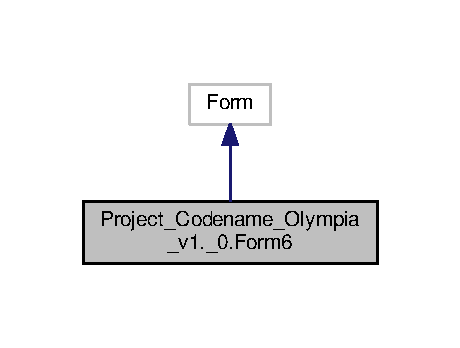
\includegraphics[width=221pt]{classProject__Codename__Olympia__v1_1_1__0_1_1Form6__inherit__graph}
\end{center}
\end{figure}


Collaboration diagram for Project\+\_\+\+Codename\+\_\+\+Olympia\+\_\+v1.\+\_\+0.\+Form6\+:
\nopagebreak
\begin{figure}[H]
\begin{center}
\leavevmode
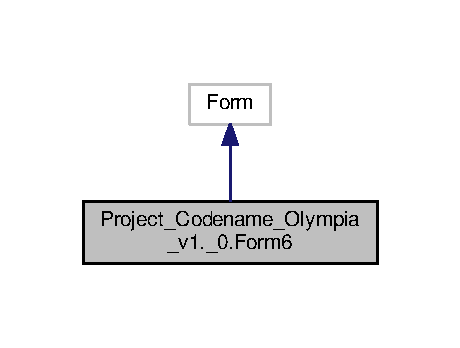
\includegraphics[width=221pt]{classProject__Codename__Olympia__v1_1_1__0_1_1Form6__coll__graph}
\end{center}
\end{figure}
\subsection*{Protected Member Functions}
\begin{DoxyCompactItemize}
\item 
override void \hyperlink{classProject__Codename__Olympia__v1_1_1__0_1_1Form6_a9136ee056a97f41d8bf4dcd25e203328}{Dispose} (bool disposing)
\begin{DoxyCompactList}\small\item\em Clean up any resources being used. \end{DoxyCompactList}\end{DoxyCompactItemize}


\subsection{Member Function Documentation}
\mbox{\Hypertarget{classProject__Codename__Olympia__v1_1_1__0_1_1Form6_a9136ee056a97f41d8bf4dcd25e203328}\label{classProject__Codename__Olympia__v1_1_1__0_1_1Form6_a9136ee056a97f41d8bf4dcd25e203328}} 
\index{Project\+\_\+\+Codename\+\_\+\+Olympia\+\_\+v1\+::\+\_\+0\+::\+Form6@{Project\+\_\+\+Codename\+\_\+\+Olympia\+\_\+v1\+::\+\_\+0\+::\+Form6}!Dispose@{Dispose}}
\index{Dispose@{Dispose}!Project\+\_\+\+Codename\+\_\+\+Olympia\+\_\+v1\+::\+\_\+0\+::\+Form6@{Project\+\_\+\+Codename\+\_\+\+Olympia\+\_\+v1\+::\+\_\+0\+::\+Form6}}
\subsubsection{\texorpdfstring{Dispose()}{Dispose()}}
{\footnotesize\ttfamily override void Project\+\_\+\+Codename\+\_\+\+Olympia\+\_\+v1.\+\_\+0.\+Form6.\+Dispose (\begin{DoxyParamCaption}\item[{bool}]{disposing }\end{DoxyParamCaption})\hspace{0.3cm}{\ttfamily [inline]}, {\ttfamily [protected]}}



Clean up any resources being used. 


\begin{DoxyParams}{Parameters}
{\em disposing} & true if managed resources should be disposed; otherwise, false.\\
\hline
\end{DoxyParams}


The documentation for this class was generated from the following files\+:\begin{DoxyCompactItemize}
\item 
Form6.\+cs\item 
Form6.\+Designer.\+cs\end{DoxyCompactItemize}

\hypertarget{classProject__Codename__Olympia__v1_1_1__0_1_1IceDance}{}\section{Project\+\_\+\+Codename\+\_\+\+Olympia\+\_\+v1.\+\_\+0.\+Ice\+Dance Class Reference}
\label{classProject__Codename__Olympia__v1_1_1__0_1_1IceDance}\index{Project\+\_\+\+Codename\+\_\+\+Olympia\+\_\+v1.\+\_\+0.\+Ice\+Dance@{Project\+\_\+\+Codename\+\_\+\+Olympia\+\_\+v1.\+\_\+0.\+Ice\+Dance}}


\hyperlink{classProject__Codename__Olympia__v1_1_1__0_1_1IceDance}{Ice\+Dance} class is one of the 3 Figure\+Skating events.  


\subsection*{Public Member Functions}
\begin{DoxyCompactItemize}
\item 
\hyperlink{classProject__Codename__Olympia__v1_1_1__0_1_1IceDance_a38ad77c543afbb217c4ba378a14a0427}{Ice\+Dance} ()
\item 
void \hyperlink{classProject__Codename__Olympia__v1_1_1__0_1_1IceDance_afc459d686d210523e2ce4a23214f4af2}{Add\+Athlete\+Male} (string country, string Fname, string Lname)
\item 
void \hyperlink{classProject__Codename__Olympia__v1_1_1__0_1_1IceDance_a528bb9a075cc030a140064ff4568eafe}{Add\+Athlete\+Female} (string country, string Fname, string Lname)
\end{DoxyCompactItemize}


\subsection{Detailed Description}
\hyperlink{classProject__Codename__Olympia__v1_1_1__0_1_1IceDance}{Ice\+Dance} class is one of the 3 Figure\+Skating events. 

D\+E\+F\+I\+N\+I\+T\+I\+ON\+: Form of figure skating where athletes participate in male/female pairs. The utilization of the same technique as Pair Skating is present but the dancing is all done in tandem versus implementing technical tricks.

C\+O\+N\+S\+T\+R\+A\+I\+N\+TS\+: The pairs are male/female. Each pair performs solo on the rink at a given time. Total duration of performance is 4 mintues and 30 seconds.\begin{DoxyAuthor}{Author}
Landen Marchand 
\end{DoxyAuthor}


\subsection{Constructor \& Destructor Documentation}
\mbox{\Hypertarget{classProject__Codename__Olympia__v1_1_1__0_1_1IceDance_a38ad77c543afbb217c4ba378a14a0427}\label{classProject__Codename__Olympia__v1_1_1__0_1_1IceDance_a38ad77c543afbb217c4ba378a14a0427}} 
\index{Project\+\_\+\+Codename\+\_\+\+Olympia\+\_\+v1\+::\+\_\+0\+::\+Ice\+Dance@{Project\+\_\+\+Codename\+\_\+\+Olympia\+\_\+v1\+::\+\_\+0\+::\+Ice\+Dance}!Ice\+Dance@{Ice\+Dance}}
\index{Ice\+Dance@{Ice\+Dance}!Project\+\_\+\+Codename\+\_\+\+Olympia\+\_\+v1\+::\+\_\+0\+::\+Ice\+Dance@{Project\+\_\+\+Codename\+\_\+\+Olympia\+\_\+v1\+::\+\_\+0\+::\+Ice\+Dance}}
\subsubsection{\texorpdfstring{Ice\+Dance()}{IceDance()}}
{\footnotesize\ttfamily Project\+\_\+\+Codename\+\_\+\+Olympia\+\_\+v1.\+\_\+0.\+Ice\+Dance.\+Ice\+Dance (\begin{DoxyParamCaption}{ }\end{DoxyParamCaption})\hspace{0.3cm}{\ttfamily [inline]}}

Default Constructor Provided Automatically 
\begin{DoxyParams}{Parameters}
{\em None} & \\
\hline
\end{DoxyParams}
\begin{DoxyReturn}{Returns}
Default Values 
\end{DoxyReturn}


\subsection{Member Function Documentation}
\mbox{\Hypertarget{classProject__Codename__Olympia__v1_1_1__0_1_1IceDance_a528bb9a075cc030a140064ff4568eafe}\label{classProject__Codename__Olympia__v1_1_1__0_1_1IceDance_a528bb9a075cc030a140064ff4568eafe}} 
\index{Project\+\_\+\+Codename\+\_\+\+Olympia\+\_\+v1\+::\+\_\+0\+::\+Ice\+Dance@{Project\+\_\+\+Codename\+\_\+\+Olympia\+\_\+v1\+::\+\_\+0\+::\+Ice\+Dance}!Add\+Athlete\+Female@{Add\+Athlete\+Female}}
\index{Add\+Athlete\+Female@{Add\+Athlete\+Female}!Project\+\_\+\+Codename\+\_\+\+Olympia\+\_\+v1\+::\+\_\+0\+::\+Ice\+Dance@{Project\+\_\+\+Codename\+\_\+\+Olympia\+\_\+v1\+::\+\_\+0\+::\+Ice\+Dance}}
\subsubsection{\texorpdfstring{Add\+Athlete\+Female()}{AddAthleteFemale()}}
{\footnotesize\ttfamily void Project\+\_\+\+Codename\+\_\+\+Olympia\+\_\+v1.\+\_\+0.\+Ice\+Dance.\+Add\+Athlete\+Female (\begin{DoxyParamCaption}\item[{string}]{country,  }\item[{string}]{Fname,  }\item[{string}]{Lname }\end{DoxyParamCaption})\hspace{0.3cm}{\ttfamily [inline]}}

Void function adds female to database for the event 
\begin{DoxyParams}{Parameters}
{\em string} & for athlete\textquotesingle{}s team name \\
\hline
{\em string} & for first name of athlete \\
\hline
{\em string} & for last name of athlete \\
\hline
\end{DoxyParams}
$<$ Creates variable for connection string

$<$ Opens DB

$<$ Checks connection and fills grid view with Race table

$<$ Adds entry to athlete information

$<$ Opens DB

$<$ Checks connection and fills grid view with Race table

$<$ Adds entry to athlete information \mbox{\Hypertarget{classProject__Codename__Olympia__v1_1_1__0_1_1IceDance_afc459d686d210523e2ce4a23214f4af2}\label{classProject__Codename__Olympia__v1_1_1__0_1_1IceDance_afc459d686d210523e2ce4a23214f4af2}} 
\index{Project\+\_\+\+Codename\+\_\+\+Olympia\+\_\+v1\+::\+\_\+0\+::\+Ice\+Dance@{Project\+\_\+\+Codename\+\_\+\+Olympia\+\_\+v1\+::\+\_\+0\+::\+Ice\+Dance}!Add\+Athlete\+Male@{Add\+Athlete\+Male}}
\index{Add\+Athlete\+Male@{Add\+Athlete\+Male}!Project\+\_\+\+Codename\+\_\+\+Olympia\+\_\+v1\+::\+\_\+0\+::\+Ice\+Dance@{Project\+\_\+\+Codename\+\_\+\+Olympia\+\_\+v1\+::\+\_\+0\+::\+Ice\+Dance}}
\subsubsection{\texorpdfstring{Add\+Athlete\+Male()}{AddAthleteMale()}}
{\footnotesize\ttfamily void Project\+\_\+\+Codename\+\_\+\+Olympia\+\_\+v1.\+\_\+0.\+Ice\+Dance.\+Add\+Athlete\+Male (\begin{DoxyParamCaption}\item[{string}]{country,  }\item[{string}]{Fname,  }\item[{string}]{Lname }\end{DoxyParamCaption})\hspace{0.3cm}{\ttfamily [inline]}}

Void function adds male to database for the event 
\begin{DoxyParams}{Parameters}
{\em string} & for athlete\textquotesingle{}s team name \\
\hline
{\em string} & for first name of athlete \\
\hline
{\em string} & for last name of athlete \\
\hline
\end{DoxyParams}
$<$ Creates variable for connection string

$<$ Opens DB

$<$ Checks connection and fills grid view with Race table

$<$ Adds entry to athlete information

$<$ Opens DB

$<$ Checks connection and fills grid view with Race table

$<$ Adds entry to athlete information 

The documentation for this class was generated from the following file\+:\begin{DoxyCompactItemize}
\item 
\hyperlink{Class1_8cs}{Class1.\+cs}\end{DoxyCompactItemize}

\hypertarget{classProject__Codename__Olympia__v1_1_1__0_1_1Judge}{}\section{Project\+\_\+\+Codename\+\_\+\+Olympia\+\_\+v1.\+\_\+0.\+Judge Class Reference}
\label{classProject__Codename__Olympia__v1_1_1__0_1_1Judge}\index{Project\+\_\+\+Codename\+\_\+\+Olympia\+\_\+v1.\+\_\+0.\+Judge@{Project\+\_\+\+Codename\+\_\+\+Olympia\+\_\+v1.\+\_\+0.\+Judge}}


\hyperlink{classProject__Codename__Olympia__v1_1_1__0_1_1Judge}{Judge} class houses and disperses all the qualified judges.  


\subsection*{Public Member Functions}
\begin{DoxyCompactItemize}
\item 
\hyperlink{classProject__Codename__Olympia__v1_1_1__0_1_1Judge_a9960078c62261a1ed3b91297fcd8ef92}{Judge} ()
\end{DoxyCompactItemize}
\subsection*{Properties}
\begin{DoxyCompactItemize}
\item 
int \hyperlink{classProject__Codename__Olympia__v1_1_1__0_1_1Judge_a7cdcda330f37b5615e86a6988a7f4738}{judge\+ID}\hspace{0.3cm}{\ttfamily  \mbox{[}get, set\mbox{]}}
\item 
\hyperlink{classProject__Codename__Olympia__v1_1_1__0_1_1Schedule}{Schedule} \hyperlink{classProject__Codename__Olympia__v1_1_1__0_1_1Judge_abc5270ee3b5cee8413bba169b17d899a}{judge\+Schedule}\hspace{0.3cm}{\ttfamily  \mbox{[}get, set\mbox{]}}
\item 
\hyperlink{classProject__Codename__Olympia__v1_1_1__0_1_1Scoring}{Scoring} \hyperlink{classProject__Codename__Olympia__v1_1_1__0_1_1Judge_a5a378d0788d1077151cd42d122aee0bc}{judge\+Score}\hspace{0.3cm}{\ttfamily  \mbox{[}get, set\mbox{]}}
\end{DoxyCompactItemize}


\subsection{Detailed Description}
\hyperlink{classProject__Codename__Olympia__v1_1_1__0_1_1Judge}{Judge} class houses and disperses all the qualified judges. 

D\+E\+F\+I\+N\+T\+I\+ON\+: A qualified person to score and assess each event. A judge is independent of all teams and free of any bias.

C\+O\+N\+S\+T\+R\+A\+I\+N\+TS\+: Provides a score ranging from 0 through 100 on scored events. Verifies accurate timing on timed events. Remains corruption-\/ free and has no contact with athletes.\begin{DoxyAuthor}{Author}
Landen Marchand 
\end{DoxyAuthor}


\subsection{Constructor \& Destructor Documentation}
\mbox{\Hypertarget{classProject__Codename__Olympia__v1_1_1__0_1_1Judge_a9960078c62261a1ed3b91297fcd8ef92}\label{classProject__Codename__Olympia__v1_1_1__0_1_1Judge_a9960078c62261a1ed3b91297fcd8ef92}} 
\index{Project\+\_\+\+Codename\+\_\+\+Olympia\+\_\+v1\+::\+\_\+0\+::\+Judge@{Project\+\_\+\+Codename\+\_\+\+Olympia\+\_\+v1\+::\+\_\+0\+::\+Judge}!Judge@{Judge}}
\index{Judge@{Judge}!Project\+\_\+\+Codename\+\_\+\+Olympia\+\_\+v1\+::\+\_\+0\+::\+Judge@{Project\+\_\+\+Codename\+\_\+\+Olympia\+\_\+v1\+::\+\_\+0\+::\+Judge}}
\subsubsection{\texorpdfstring{Judge()}{Judge()}}
{\footnotesize\ttfamily Project\+\_\+\+Codename\+\_\+\+Olympia\+\_\+v1.\+\_\+0.\+Judge.\+Judge (\begin{DoxyParamCaption}{ }\end{DoxyParamCaption})\hspace{0.3cm}{\ttfamily [inline]}}

Default Constructor Provided Automatically 
\begin{DoxyParams}{Parameters}
{\em None} & \\
\hline
\end{DoxyParams}
\begin{DoxyReturn}{Returns}
Default Values 
\end{DoxyReturn}


\subsection{Property Documentation}
\mbox{\Hypertarget{classProject__Codename__Olympia__v1_1_1__0_1_1Judge_a7cdcda330f37b5615e86a6988a7f4738}\label{classProject__Codename__Olympia__v1_1_1__0_1_1Judge_a7cdcda330f37b5615e86a6988a7f4738}} 
\index{Project\+\_\+\+Codename\+\_\+\+Olympia\+\_\+v1\+::\+\_\+0\+::\+Judge@{Project\+\_\+\+Codename\+\_\+\+Olympia\+\_\+v1\+::\+\_\+0\+::\+Judge}!judge\+ID@{judge\+ID}}
\index{judge\+ID@{judge\+ID}!Project\+\_\+\+Codename\+\_\+\+Olympia\+\_\+v1\+::\+\_\+0\+::\+Judge@{Project\+\_\+\+Codename\+\_\+\+Olympia\+\_\+v1\+::\+\_\+0\+::\+Judge}}
\subsubsection{\texorpdfstring{judge\+ID}{judgeID}}
{\footnotesize\ttfamily int Project\+\_\+\+Codename\+\_\+\+Olympia\+\_\+v1.\+\_\+0.\+Judge.\+judge\+ID\hspace{0.3cm}{\ttfamily [get]}, {\ttfamily [set]}}

Sets and gets judge\textquotesingle{}s ID number 
\begin{DoxyParams}{Parameters}
{\em int} & for ID number \\
\hline
\end{DoxyParams}
\begin{DoxyReturn}{Returns}
int ID number 
\end{DoxyReturn}
\mbox{\Hypertarget{classProject__Codename__Olympia__v1_1_1__0_1_1Judge_abc5270ee3b5cee8413bba169b17d899a}\label{classProject__Codename__Olympia__v1_1_1__0_1_1Judge_abc5270ee3b5cee8413bba169b17d899a}} 
\index{Project\+\_\+\+Codename\+\_\+\+Olympia\+\_\+v1\+::\+\_\+0\+::\+Judge@{Project\+\_\+\+Codename\+\_\+\+Olympia\+\_\+v1\+::\+\_\+0\+::\+Judge}!judge\+Schedule@{judge\+Schedule}}
\index{judge\+Schedule@{judge\+Schedule}!Project\+\_\+\+Codename\+\_\+\+Olympia\+\_\+v1\+::\+\_\+0\+::\+Judge@{Project\+\_\+\+Codename\+\_\+\+Olympia\+\_\+v1\+::\+\_\+0\+::\+Judge}}
\subsubsection{\texorpdfstring{judge\+Schedule}{judgeSchedule}}
{\footnotesize\ttfamily \hyperlink{classProject__Codename__Olympia__v1_1_1__0_1_1Schedule}{Schedule} Project\+\_\+\+Codename\+\_\+\+Olympia\+\_\+v1.\+\_\+0.\+Judge.\+judge\+Schedule\hspace{0.3cm}{\ttfamily [get]}, {\ttfamily [set]}}

Sets and gets the schedule for each judge 
\begin{DoxyParams}{Parameters}
{\em \hyperlink{classProject__Codename__Olympia__v1_1_1__0_1_1Schedule}{Schedule}} & \\
\hline
\end{DoxyParams}
\begin{DoxyReturn}{Returns}
\hyperlink{classProject__Codename__Olympia__v1_1_1__0_1_1Schedule}{Schedule} 
\end{DoxyReturn}
\mbox{\Hypertarget{classProject__Codename__Olympia__v1_1_1__0_1_1Judge_a5a378d0788d1077151cd42d122aee0bc}\label{classProject__Codename__Olympia__v1_1_1__0_1_1Judge_a5a378d0788d1077151cd42d122aee0bc}} 
\index{Project\+\_\+\+Codename\+\_\+\+Olympia\+\_\+v1\+::\+\_\+0\+::\+Judge@{Project\+\_\+\+Codename\+\_\+\+Olympia\+\_\+v1\+::\+\_\+0\+::\+Judge}!judge\+Score@{judge\+Score}}
\index{judge\+Score@{judge\+Score}!Project\+\_\+\+Codename\+\_\+\+Olympia\+\_\+v1\+::\+\_\+0\+::\+Judge@{Project\+\_\+\+Codename\+\_\+\+Olympia\+\_\+v1\+::\+\_\+0\+::\+Judge}}
\subsubsection{\texorpdfstring{judge\+Score}{judgeScore}}
{\footnotesize\ttfamily \hyperlink{classProject__Codename__Olympia__v1_1_1__0_1_1Scoring}{Scoring} Project\+\_\+\+Codename\+\_\+\+Olympia\+\_\+v1.\+\_\+0.\+Judge.\+judge\+Score\hspace{0.3cm}{\ttfamily [get]}, {\ttfamily [set]}}

Sets and gets the score for each event 
\begin{DoxyParams}{Parameters}
{\em \hyperlink{classProject__Codename__Olympia__v1_1_1__0_1_1Scoring}{Scoring}} & \\
\hline
\end{DoxyParams}
\begin{DoxyReturn}{Returns}
\hyperlink{classProject__Codename__Olympia__v1_1_1__0_1_1Scoring}{Scoring} 
\end{DoxyReturn}


The documentation for this class was generated from the following file\+:\begin{DoxyCompactItemize}
\item 
Class1.\+cs\end{DoxyCompactItemize}

\hypertarget{classProject__Codename__Olympia__v1_1_1__0_1_1PairSkating}{}\section{Project\+\_\+\+Codename\+\_\+\+Olympia\+\_\+v1.\+\_\+0.\+Pair\+Skating Class Reference}
\label{classProject__Codename__Olympia__v1_1_1__0_1_1PairSkating}\index{Project\+\_\+\+Codename\+\_\+\+Olympia\+\_\+v1.\+\_\+0.\+Pair\+Skating@{Project\+\_\+\+Codename\+\_\+\+Olympia\+\_\+v1.\+\_\+0.\+Pair\+Skating}}


\hyperlink{classProject__Codename__Olympia__v1_1_1__0_1_1PairSkating}{Pair\+Skating} class is one of the 3 \hyperlink{classProject__Codename__Olympia__v1_1_1__0_1_1FigureSkating}{Figure\+Skating} events.  




Inheritance diagram for Project\+\_\+\+Codename\+\_\+\+Olympia\+\_\+v1.\+\_\+0.\+Pair\+Skating\+:
\nopagebreak
\begin{figure}[H]
\begin{center}
\leavevmode
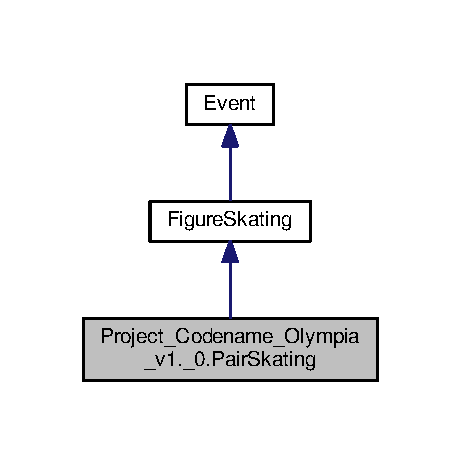
\includegraphics[width=221pt]{classProject__Codename__Olympia__v1_1_1__0_1_1PairSkating__inherit__graph}
\end{center}
\end{figure}


Collaboration diagram for Project\+\_\+\+Codename\+\_\+\+Olympia\+\_\+v1.\+\_\+0.\+Pair\+Skating\+:
\nopagebreak
\begin{figure}[H]
\begin{center}
\leavevmode
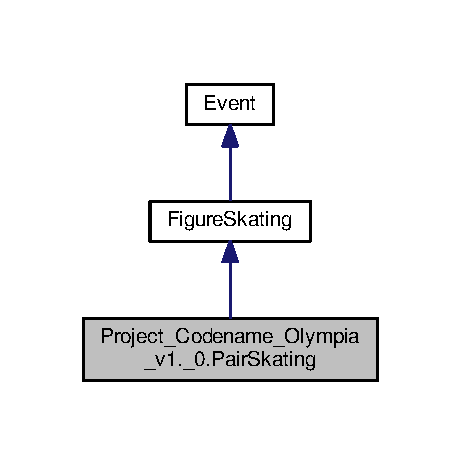
\includegraphics[width=221pt]{classProject__Codename__Olympia__v1_1_1__0_1_1PairSkating__coll__graph}
\end{center}
\end{figure}
\subsection*{Public Member Functions}
\begin{DoxyCompactItemize}
\item 
\hyperlink{classProject__Codename__Olympia__v1_1_1__0_1_1PairSkating_aac71e0374562ef7e4c3d9c87366517f9}{Pair\+Skating} ()
\item 
override double \hyperlink{classProject__Codename__Olympia__v1_1_1__0_1_1PairSkating_aef6f7313446386c4e6bdf8a438e246a1}{fs\+Score} ()
\item 
override int \hyperlink{classProject__Codename__Olympia__v1_1_1__0_1_1PairSkating_a22c797f9392cc5e53c9cbacb641e56e0}{event\+Num} ()
\item 
override void \hyperlink{classProject__Codename__Olympia__v1_1_1__0_1_1PairSkating_a5150348cf16352d2ce4ae63ac4e8a44d}{run\+Event} (List$<$ \hyperlink{classProject__Codename__Olympia__v1_1_1__0_1_1Judge}{Judge} $>$ j, List$<$ \hyperlink{classProject__Codename__Olympia__v1_1_1__0_1_1Team}{Team} $>$ t)
\item 
override void \hyperlink{classProject__Codename__Olympia__v1_1_1__0_1_1PairSkating_abc9c2d9765ad831e59228697a334da6d}{sched\+Event} (List$<$ \hyperlink{classProject__Codename__Olympia__v1_1_1__0_1_1Judge}{Judge} $>$ j, List$<$ \hyperlink{classProject__Codename__Olympia__v1_1_1__0_1_1Team}{Team} $>$ t)
\end{DoxyCompactItemize}


\subsection{Detailed Description}
\hyperlink{classProject__Codename__Olympia__v1_1_1__0_1_1PairSkating}{Pair\+Skating} class is one of the 3 \hyperlink{classProject__Codename__Olympia__v1_1_1__0_1_1FigureSkating}{Figure\+Skating} events. 

D\+E\+F\+I\+N\+I\+T\+I\+ON\+: Form of figure skating where athletes participate in male/female pairs. The utilization of long program style where each athlete is free to do their own unique performance complete with technical tricks is present.

C\+O\+N\+S\+T\+R\+A\+I\+N\+TS\+: The pairs are male female. Each pair performs solo on the rink at a given time. Total duration of performance is 4 mintues and 30 seconds.\begin{DoxyAuthor}{Author}
Landen Marchand 
\end{DoxyAuthor}


\subsection{Constructor \& Destructor Documentation}
\mbox{\Hypertarget{classProject__Codename__Olympia__v1_1_1__0_1_1PairSkating_aac71e0374562ef7e4c3d9c87366517f9}\label{classProject__Codename__Olympia__v1_1_1__0_1_1PairSkating_aac71e0374562ef7e4c3d9c87366517f9}} 
\index{Project\+\_\+\+Codename\+\_\+\+Olympia\+\_\+v1\+::\+\_\+0\+::\+Pair\+Skating@{Project\+\_\+\+Codename\+\_\+\+Olympia\+\_\+v1\+::\+\_\+0\+::\+Pair\+Skating}!Pair\+Skating@{Pair\+Skating}}
\index{Pair\+Skating@{Pair\+Skating}!Project\+\_\+\+Codename\+\_\+\+Olympia\+\_\+v1\+::\+\_\+0\+::\+Pair\+Skating@{Project\+\_\+\+Codename\+\_\+\+Olympia\+\_\+v1\+::\+\_\+0\+::\+Pair\+Skating}}
\subsubsection{\texorpdfstring{Pair\+Skating()}{PairSkating()}}
{\footnotesize\ttfamily Project\+\_\+\+Codename\+\_\+\+Olympia\+\_\+v1.\+\_\+0.\+Pair\+Skating.\+Pair\+Skating (\begin{DoxyParamCaption}{ }\end{DoxyParamCaption})\hspace{0.3cm}{\ttfamily [inline]}}

Default Constructor Provided Automatically 
\begin{DoxyParams}{Parameters}
{\em None} & \\
\hline
\end{DoxyParams}
\begin{DoxyReturn}{Returns}
Default Values 
\end{DoxyReturn}


\subsection{Member Function Documentation}
\mbox{\Hypertarget{classProject__Codename__Olympia__v1_1_1__0_1_1PairSkating_a22c797f9392cc5e53c9cbacb641e56e0}\label{classProject__Codename__Olympia__v1_1_1__0_1_1PairSkating_a22c797f9392cc5e53c9cbacb641e56e0}} 
\index{Project\+\_\+\+Codename\+\_\+\+Olympia\+\_\+v1\+::\+\_\+0\+::\+Pair\+Skating@{Project\+\_\+\+Codename\+\_\+\+Olympia\+\_\+v1\+::\+\_\+0\+::\+Pair\+Skating}!event\+Num@{event\+Num}}
\index{event\+Num@{event\+Num}!Project\+\_\+\+Codename\+\_\+\+Olympia\+\_\+v1\+::\+\_\+0\+::\+Pair\+Skating@{Project\+\_\+\+Codename\+\_\+\+Olympia\+\_\+v1\+::\+\_\+0\+::\+Pair\+Skating}}
\subsubsection{\texorpdfstring{event\+Num()}{eventNum()}}
{\footnotesize\ttfamily override int Project\+\_\+\+Codename\+\_\+\+Olympia\+\_\+v1.\+\_\+0.\+Pair\+Skating.\+event\+Num (\begin{DoxyParamCaption}{ }\end{DoxyParamCaption})\hspace{0.3cm}{\ttfamily [inline]}, {\ttfamily [virtual]}}

Function to override inherited \hyperlink{classProject__Codename__Olympia__v1_1_1__0_1_1PairSkating_a22c797f9392cc5e53c9cbacb641e56e0}{event\+Num()} function 

Implements \hyperlink{classProject__Codename__Olympia__v1_1_1__0_1_1Event_ad1154ef4dd1dec29d8ebf5614d84b1f3}{Project\+\_\+\+Codename\+\_\+\+Olympia\+\_\+v1.\+\_\+0.\+Event}.

\mbox{\Hypertarget{classProject__Codename__Olympia__v1_1_1__0_1_1PairSkating_aef6f7313446386c4e6bdf8a438e246a1}\label{classProject__Codename__Olympia__v1_1_1__0_1_1PairSkating_aef6f7313446386c4e6bdf8a438e246a1}} 
\index{Project\+\_\+\+Codename\+\_\+\+Olympia\+\_\+v1\+::\+\_\+0\+::\+Pair\+Skating@{Project\+\_\+\+Codename\+\_\+\+Olympia\+\_\+v1\+::\+\_\+0\+::\+Pair\+Skating}!fs\+Score@{fs\+Score}}
\index{fs\+Score@{fs\+Score}!Project\+\_\+\+Codename\+\_\+\+Olympia\+\_\+v1\+::\+\_\+0\+::\+Pair\+Skating@{Project\+\_\+\+Codename\+\_\+\+Olympia\+\_\+v1\+::\+\_\+0\+::\+Pair\+Skating}}
\subsubsection{\texorpdfstring{fs\+Score()}{fsScore()}}
{\footnotesize\ttfamily override double Project\+\_\+\+Codename\+\_\+\+Olympia\+\_\+v1.\+\_\+0.\+Pair\+Skating.\+fs\+Score (\begin{DoxyParamCaption}{ }\end{DoxyParamCaption})\hspace{0.3cm}{\ttfamily [inline]}, {\ttfamily [virtual]}}

Function to override inherited \hyperlink{classProject__Codename__Olympia__v1_1_1__0_1_1PairSkating_aef6f7313446386c4e6bdf8a438e246a1}{fs\+Score()} function 

Implements \hyperlink{classProject__Codename__Olympia__v1_1_1__0_1_1FigureSkating_a437e794fec382863421f8c65e31295f8}{Project\+\_\+\+Codename\+\_\+\+Olympia\+\_\+v1.\+\_\+0.\+Figure\+Skating}.

\mbox{\Hypertarget{classProject__Codename__Olympia__v1_1_1__0_1_1PairSkating_a5150348cf16352d2ce4ae63ac4e8a44d}\label{classProject__Codename__Olympia__v1_1_1__0_1_1PairSkating_a5150348cf16352d2ce4ae63ac4e8a44d}} 
\index{Project\+\_\+\+Codename\+\_\+\+Olympia\+\_\+v1\+::\+\_\+0\+::\+Pair\+Skating@{Project\+\_\+\+Codename\+\_\+\+Olympia\+\_\+v1\+::\+\_\+0\+::\+Pair\+Skating}!run\+Event@{run\+Event}}
\index{run\+Event@{run\+Event}!Project\+\_\+\+Codename\+\_\+\+Olympia\+\_\+v1\+::\+\_\+0\+::\+Pair\+Skating@{Project\+\_\+\+Codename\+\_\+\+Olympia\+\_\+v1\+::\+\_\+0\+::\+Pair\+Skating}}
\subsubsection{\texorpdfstring{run\+Event()}{runEvent()}}
{\footnotesize\ttfamily override void Project\+\_\+\+Codename\+\_\+\+Olympia\+\_\+v1.\+\_\+0.\+Pair\+Skating.\+run\+Event (\begin{DoxyParamCaption}\item[{List$<$ \hyperlink{classProject__Codename__Olympia__v1_1_1__0_1_1Judge}{Judge} $>$}]{j,  }\item[{List$<$ \hyperlink{classProject__Codename__Olympia__v1_1_1__0_1_1Team}{Team} $>$}]{t }\end{DoxyParamCaption})\hspace{0.3cm}{\ttfamily [inline]}, {\ttfamily [virtual]}}

Function to override inherited run\+Event(..) function 

Implements \hyperlink{classProject__Codename__Olympia__v1_1_1__0_1_1Event_ac6ff060da23153c02da49937dcf9f326}{Project\+\_\+\+Codename\+\_\+\+Olympia\+\_\+v1.\+\_\+0.\+Event}.

\mbox{\Hypertarget{classProject__Codename__Olympia__v1_1_1__0_1_1PairSkating_abc9c2d9765ad831e59228697a334da6d}\label{classProject__Codename__Olympia__v1_1_1__0_1_1PairSkating_abc9c2d9765ad831e59228697a334da6d}} 
\index{Project\+\_\+\+Codename\+\_\+\+Olympia\+\_\+v1\+::\+\_\+0\+::\+Pair\+Skating@{Project\+\_\+\+Codename\+\_\+\+Olympia\+\_\+v1\+::\+\_\+0\+::\+Pair\+Skating}!sched\+Event@{sched\+Event}}
\index{sched\+Event@{sched\+Event}!Project\+\_\+\+Codename\+\_\+\+Olympia\+\_\+v1\+::\+\_\+0\+::\+Pair\+Skating@{Project\+\_\+\+Codename\+\_\+\+Olympia\+\_\+v1\+::\+\_\+0\+::\+Pair\+Skating}}
\subsubsection{\texorpdfstring{sched\+Event()}{schedEvent()}}
{\footnotesize\ttfamily override void Project\+\_\+\+Codename\+\_\+\+Olympia\+\_\+v1.\+\_\+0.\+Pair\+Skating.\+sched\+Event (\begin{DoxyParamCaption}\item[{List$<$ \hyperlink{classProject__Codename__Olympia__v1_1_1__0_1_1Judge}{Judge} $>$}]{j,  }\item[{List$<$ \hyperlink{classProject__Codename__Olympia__v1_1_1__0_1_1Team}{Team} $>$}]{t }\end{DoxyParamCaption})\hspace{0.3cm}{\ttfamily [inline]}, {\ttfamily [virtual]}}

Function to override inherited sched\+Event(..) function 

Implements \hyperlink{classProject__Codename__Olympia__v1_1_1__0_1_1Event_abb4e2b9c28527b9a28395f2fe9192196}{Project\+\_\+\+Codename\+\_\+\+Olympia\+\_\+v1.\+\_\+0.\+Event}.



The documentation for this class was generated from the following file\+:\begin{DoxyCompactItemize}
\item 
Class1.\+cs\end{DoxyCompactItemize}

\hypertarget{classProject__Codename__Olympia__v1_1_1__0_1_1RegisterEventForm}{}\section{Project\+\_\+\+Codename\+\_\+\+Olympia\+\_\+v1.\+\_\+0.\+Register\+Event\+Form Class Reference}
\label{classProject__Codename__Olympia__v1_1_1__0_1_1RegisterEventForm}\index{Project\+\_\+\+Codename\+\_\+\+Olympia\+\_\+v1.\+\_\+0.\+Register\+Event\+Form@{Project\+\_\+\+Codename\+\_\+\+Olympia\+\_\+v1.\+\_\+0.\+Register\+Event\+Form}}


Inheritance diagram for Project\+\_\+\+Codename\+\_\+\+Olympia\+\_\+v1.\+\_\+0.\+Register\+Event\+Form\+:
\nopagebreak
\begin{figure}[H]
\begin{center}
\leavevmode
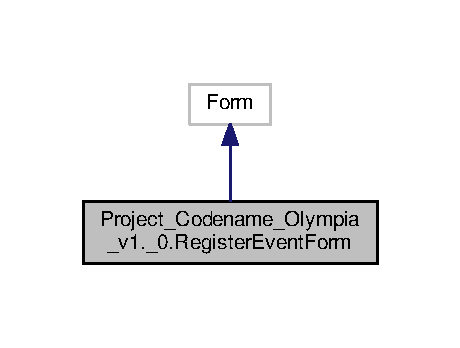
\includegraphics[width=221pt]{classProject__Codename__Olympia__v1_1_1__0_1_1RegisterEventForm__inherit__graph}
\end{center}
\end{figure}


Collaboration diagram for Project\+\_\+\+Codename\+\_\+\+Olympia\+\_\+v1.\+\_\+0.\+Register\+Event\+Form\+:
\nopagebreak
\begin{figure}[H]
\begin{center}
\leavevmode
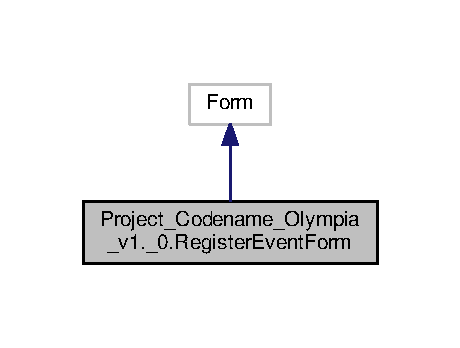
\includegraphics[width=221pt]{classProject__Codename__Olympia__v1_1_1__0_1_1RegisterEventForm__coll__graph}
\end{center}
\end{figure}
\subsection*{Protected Member Functions}
\begin{DoxyCompactItemize}
\item 
override void \hyperlink{classProject__Codename__Olympia__v1_1_1__0_1_1RegisterEventForm_a36314720f560074be6a7a2fa7bde5cbe}{Dispose} (bool disposing)
\begin{DoxyCompactList}\small\item\em Clean up any resources being used. \end{DoxyCompactList}\end{DoxyCompactItemize}


\subsection{Member Function Documentation}
\mbox{\Hypertarget{classProject__Codename__Olympia__v1_1_1__0_1_1RegisterEventForm_a36314720f560074be6a7a2fa7bde5cbe}\label{classProject__Codename__Olympia__v1_1_1__0_1_1RegisterEventForm_a36314720f560074be6a7a2fa7bde5cbe}} 
\index{Project\+\_\+\+Codename\+\_\+\+Olympia\+\_\+v1\+::\+\_\+0\+::\+Register\+Event\+Form@{Project\+\_\+\+Codename\+\_\+\+Olympia\+\_\+v1\+::\+\_\+0\+::\+Register\+Event\+Form}!Dispose@{Dispose}}
\index{Dispose@{Dispose}!Project\+\_\+\+Codename\+\_\+\+Olympia\+\_\+v1\+::\+\_\+0\+::\+Register\+Event\+Form@{Project\+\_\+\+Codename\+\_\+\+Olympia\+\_\+v1\+::\+\_\+0\+::\+Register\+Event\+Form}}
\subsubsection{\texorpdfstring{Dispose()}{Dispose()}}
{\footnotesize\ttfamily override void Project\+\_\+\+Codename\+\_\+\+Olympia\+\_\+v1.\+\_\+0.\+Register\+Event\+Form.\+Dispose (\begin{DoxyParamCaption}\item[{bool}]{disposing }\end{DoxyParamCaption})\hspace{0.3cm}{\ttfamily [inline]}, {\ttfamily [protected]}}



Clean up any resources being used. 


\begin{DoxyParams}{Parameters}
{\em disposing} & true if managed resources should be disposed; otherwise, false.\\
\hline
\end{DoxyParams}


The documentation for this class was generated from the following files\+:\begin{DoxyCompactItemize}
\item 
Form4.\+cs\item 
Form4.\+Designer.\+cs\end{DoxyCompactItemize}

\hypertarget{classProject__Codename__Olympia__v1_1_1__0_1_1Registration}{}\section{Project\+\_\+\+Codename\+\_\+\+Olympia\+\_\+v1.\+\_\+0.\+Registration Class Reference}
\label{classProject__Codename__Olympia__v1_1_1__0_1_1Registration}\index{Project\+\_\+\+Codename\+\_\+\+Olympia\+\_\+v1.\+\_\+0.\+Registration@{Project\+\_\+\+Codename\+\_\+\+Olympia\+\_\+v1.\+\_\+0.\+Registration}}


\hyperlink{classProject__Codename__Olympia__v1_1_1__0_1_1Registration}{Registration} class registers Teams and Athletes.  


\subsection*{Public Member Functions}
\begin{DoxyCompactItemize}
\item 
\hyperlink{classProject__Codename__Olympia__v1_1_1__0_1_1Registration_a1c89ef8d19a30a89a298d540f576f146}{Registration} ()
\item 
List$<$ \hyperlink{classProject__Codename__Olympia__v1_1_1__0_1_1Team}{Team} $>$ \hyperlink{classProject__Codename__Olympia__v1_1_1__0_1_1Registration_a44b2f6bdcf9dbd46d155af0c8bafa2ae}{register\+Team} ()
\end{DoxyCompactItemize}


\subsection{Detailed Description}
\hyperlink{classProject__Codename__Olympia__v1_1_1__0_1_1Registration}{Registration} class registers Teams and Athletes. 

D\+E\+F\+I\+N\+T\+I\+ON\+: The process of obtaining athletes who have successfully completed all qualification rounds prior to the Winter Olympics. \hyperlink{classProject__Codename__Olympia__v1_1_1__0_1_1Registration}{Registration} places athletes into their respective team and places athletes to a specified event.

C\+O\+N\+S\+T\+R\+A\+I\+N\+TS\+: Sets a maximum limit of athletes per event. Sets a max limit on number of teams in the Winter Olympics.\begin{DoxyAuthor}{Author}
Landen Marchand 
\end{DoxyAuthor}


\subsection{Constructor \& Destructor Documentation}
\mbox{\Hypertarget{classProject__Codename__Olympia__v1_1_1__0_1_1Registration_a1c89ef8d19a30a89a298d540f576f146}\label{classProject__Codename__Olympia__v1_1_1__0_1_1Registration_a1c89ef8d19a30a89a298d540f576f146}} 
\index{Project\+\_\+\+Codename\+\_\+\+Olympia\+\_\+v1\+::\+\_\+0\+::\+Registration@{Project\+\_\+\+Codename\+\_\+\+Olympia\+\_\+v1\+::\+\_\+0\+::\+Registration}!Registration@{Registration}}
\index{Registration@{Registration}!Project\+\_\+\+Codename\+\_\+\+Olympia\+\_\+v1\+::\+\_\+0\+::\+Registration@{Project\+\_\+\+Codename\+\_\+\+Olympia\+\_\+v1\+::\+\_\+0\+::\+Registration}}
\subsubsection{\texorpdfstring{Registration()}{Registration()}}
{\footnotesize\ttfamily Project\+\_\+\+Codename\+\_\+\+Olympia\+\_\+v1.\+\_\+0.\+Registration.\+Registration (\begin{DoxyParamCaption}{ }\end{DoxyParamCaption})\hspace{0.3cm}{\ttfamily [inline]}}

Default Constructor Provided Automatically 
\begin{DoxyParams}{Parameters}
{\em None} & \\
\hline
\end{DoxyParams}
\begin{DoxyReturn}{Returns}
Default Values 
\end{DoxyReturn}


\subsection{Member Function Documentation}
\mbox{\Hypertarget{classProject__Codename__Olympia__v1_1_1__0_1_1Registration_a44b2f6bdcf9dbd46d155af0c8bafa2ae}\label{classProject__Codename__Olympia__v1_1_1__0_1_1Registration_a44b2f6bdcf9dbd46d155af0c8bafa2ae}} 
\index{Project\+\_\+\+Codename\+\_\+\+Olympia\+\_\+v1\+::\+\_\+0\+::\+Registration@{Project\+\_\+\+Codename\+\_\+\+Olympia\+\_\+v1\+::\+\_\+0\+::\+Registration}!register\+Team@{register\+Team}}
\index{register\+Team@{register\+Team}!Project\+\_\+\+Codename\+\_\+\+Olympia\+\_\+v1\+::\+\_\+0\+::\+Registration@{Project\+\_\+\+Codename\+\_\+\+Olympia\+\_\+v1\+::\+\_\+0\+::\+Registration}}
\subsubsection{\texorpdfstring{register\+Team()}{registerTeam()}}
{\footnotesize\ttfamily List$<$\hyperlink{classProject__Codename__Olympia__v1_1_1__0_1_1Team}{Team}$>$ Project\+\_\+\+Codename\+\_\+\+Olympia\+\_\+v1.\+\_\+0.\+Registration.\+register\+Team (\begin{DoxyParamCaption}{ }\end{DoxyParamCaption})\hspace{0.3cm}{\ttfamily [inline]}}

Officially enters a team into the Winter Olympics $\ast$$\ast$\+N\+O\+TE\+: T\+H\+IS W\+I\+LL BE M\+O\+D\+I\+F\+I\+ED A\+F\+T\+ER M\+O\+RE I\+N\+FO IS O\+B\+T\+A\+I\+N\+E\+D$\ast$$\ast$ 
\begin{DoxyParams}{Parameters}
{\em none} & \\
\hline
\end{DoxyParams}
\begin{DoxyReturn}{Returns}
List$<$\+Team$>$ which is the official list of all teams and their athletes 
\end{DoxyReturn}


The documentation for this class was generated from the following file\+:\begin{DoxyCompactItemize}
\item 
Class1.\+cs\end{DoxyCompactItemize}

\hypertarget{classProject__Codename__Olympia__v1_1_1__0_1_1Rink}{}\section{Project\+\_\+\+Codename\+\_\+\+Olympia\+\_\+v1.\+\_\+0.\+Rink Class Reference}
\label{classProject__Codename__Olympia__v1_1_1__0_1_1Rink}\index{Project\+\_\+\+Codename\+\_\+\+Olympia\+\_\+v1.\+\_\+0.\+Rink@{Project\+\_\+\+Codename\+\_\+\+Olympia\+\_\+v1.\+\_\+0.\+Rink}}


\hyperlink{classProject__Codename__Olympia__v1_1_1__0_1_1Rink}{Rink} class is the physical area in which events are held.  


\subsection*{Public Member Functions}
\begin{DoxyCompactItemize}
\item 
\hyperlink{classProject__Codename__Olympia__v1_1_1__0_1_1Rink_a25a7e3b332da40b6ff448203f1006063}{Rink} ()
\item 
List$<$ \hyperlink{classProject__Codename__Olympia__v1_1_1__0_1_1Event}{Event} $>$ \hyperlink{classProject__Codename__Olympia__v1_1_1__0_1_1Rink_a79363adae7214d4718bd0e6c6dde7258}{rink\+Events} ()
\end{DoxyCompactItemize}


\subsection{Detailed Description}
\hyperlink{classProject__Codename__Olympia__v1_1_1__0_1_1Rink}{Rink} class is the physical area in which events are held. 

D\+E\+F\+I\+N\+I\+T\+I\+ON\+: The location of each event determined by the schedule.

C\+O\+N\+S\+T\+R\+A\+I\+N\+TS\+: May only be occupied by one event at any given time. Must be in operation concurrent with the other rinks.\begin{DoxyAuthor}{Author}
Landen Marchand 
\end{DoxyAuthor}


\subsection{Constructor \& Destructor Documentation}
\mbox{\Hypertarget{classProject__Codename__Olympia__v1_1_1__0_1_1Rink_a25a7e3b332da40b6ff448203f1006063}\label{classProject__Codename__Olympia__v1_1_1__0_1_1Rink_a25a7e3b332da40b6ff448203f1006063}} 
\index{Project\+\_\+\+Codename\+\_\+\+Olympia\+\_\+v1\+::\+\_\+0\+::\+Rink@{Project\+\_\+\+Codename\+\_\+\+Olympia\+\_\+v1\+::\+\_\+0\+::\+Rink}!Rink@{Rink}}
\index{Rink@{Rink}!Project\+\_\+\+Codename\+\_\+\+Olympia\+\_\+v1\+::\+\_\+0\+::\+Rink@{Project\+\_\+\+Codename\+\_\+\+Olympia\+\_\+v1\+::\+\_\+0\+::\+Rink}}
\subsubsection{\texorpdfstring{Rink()}{Rink()}}
{\footnotesize\ttfamily Project\+\_\+\+Codename\+\_\+\+Olympia\+\_\+v1.\+\_\+0.\+Rink.\+Rink (\begin{DoxyParamCaption}{ }\end{DoxyParamCaption})\hspace{0.3cm}{\ttfamily [inline]}}

Default Constructor Provided Automatically 
\begin{DoxyParams}{Parameters}
{\em None} & \\
\hline
\end{DoxyParams}
\begin{DoxyReturn}{Returns}
Default Values 
\end{DoxyReturn}


\subsection{Member Function Documentation}
\mbox{\Hypertarget{classProject__Codename__Olympia__v1_1_1__0_1_1Rink_a79363adae7214d4718bd0e6c6dde7258}\label{classProject__Codename__Olympia__v1_1_1__0_1_1Rink_a79363adae7214d4718bd0e6c6dde7258}} 
\index{Project\+\_\+\+Codename\+\_\+\+Olympia\+\_\+v1\+::\+\_\+0\+::\+Rink@{Project\+\_\+\+Codename\+\_\+\+Olympia\+\_\+v1\+::\+\_\+0\+::\+Rink}!rink\+Events@{rink\+Events}}
\index{rink\+Events@{rink\+Events}!Project\+\_\+\+Codename\+\_\+\+Olympia\+\_\+v1\+::\+\_\+0\+::\+Rink@{Project\+\_\+\+Codename\+\_\+\+Olympia\+\_\+v1\+::\+\_\+0\+::\+Rink}}
\subsubsection{\texorpdfstring{rink\+Events()}{rinkEvents()}}
{\footnotesize\ttfamily List$<$\hyperlink{classProject__Codename__Olympia__v1_1_1__0_1_1Event}{Event}$>$ Project\+\_\+\+Codename\+\_\+\+Olympia\+\_\+v1.\+\_\+0.\+Rink.\+rink\+Events (\begin{DoxyParamCaption}{ }\end{DoxyParamCaption})\hspace{0.3cm}{\ttfamily [inline]}}

Function to obtain all the events that are held on a certain rink 
\begin{DoxyParams}{Parameters}
{\em none} & \\
\hline
\end{DoxyParams}
\begin{DoxyReturn}{Returns}
List$<$\+Event$>$ which is the list of all events that are held on a particular rink 
\end{DoxyReturn}


The documentation for this class was generated from the following file\+:\begin{DoxyCompactItemize}
\item 
Class1.\+cs\end{DoxyCompactItemize}

\hypertarget{classProject__Codename__Olympia__v1_1_1__0_1_1Schedule}{}\section{Project\+\_\+\+Codename\+\_\+\+Olympia\+\_\+v1.\+\_\+0.\+Schedule Class Reference}
\label{classProject__Codename__Olympia__v1_1_1__0_1_1Schedule}\index{Project\+\_\+\+Codename\+\_\+\+Olympia\+\_\+v1.\+\_\+0.\+Schedule@{Project\+\_\+\+Codename\+\_\+\+Olympia\+\_\+v1.\+\_\+0.\+Schedule}}


\hyperlink{classProject__Codename__Olympia__v1_1_1__0_1_1Schedule}{Schedule} class is the organization of athletes and events.  


\subsection*{Public Member Functions}
\begin{DoxyCompactItemize}
\item 
\hyperlink{classProject__Codename__Olympia__v1_1_1__0_1_1Schedule_af4fe4aaff507c77bfc5294025b8342c2}{Schedule} ()
\end{DoxyCompactItemize}
\subsection*{Properties}
\begin{DoxyCompactItemize}
\item 
List$<$ Tuple$<$ int, int $>$ $>$ \hyperlink{classProject__Codename__Olympia__v1_1_1__0_1_1Schedule_a1aabf7243a96c19b51b2cb482b6ef421}{event\+Scheduler}\hspace{0.3cm}{\ttfamily  \mbox{[}get, set\mbox{]}}
\end{DoxyCompactItemize}


\subsection{Detailed Description}
\hyperlink{classProject__Codename__Olympia__v1_1_1__0_1_1Schedule}{Schedule} class is the organization of athletes and events. 

D\+E\+F\+I\+N\+T\+I\+ON\+: The chronological listing of events over the course of two weeks. Scheduling implements where and when events are held. \hyperlink{classProject__Codename__Olympia__v1_1_1__0_1_1Schedule}{Schedule} is also the organization of athletes placed into their respective events.

C\+O\+N\+S\+T\+R\+A\+I\+N\+TS\+: Must not organize events such that they happen concurrently on the same rink. Must not allot more than the appropriate amount of athletes per event. Must make sure any event is done as a pair contains one male and one female athlete per team.\begin{DoxyAuthor}{Author}
Landen Marchand 
\end{DoxyAuthor}


\subsection{Constructor \& Destructor Documentation}
\mbox{\Hypertarget{classProject__Codename__Olympia__v1_1_1__0_1_1Schedule_af4fe4aaff507c77bfc5294025b8342c2}\label{classProject__Codename__Olympia__v1_1_1__0_1_1Schedule_af4fe4aaff507c77bfc5294025b8342c2}} 
\index{Project\+\_\+\+Codename\+\_\+\+Olympia\+\_\+v1\+::\+\_\+0\+::\+Schedule@{Project\+\_\+\+Codename\+\_\+\+Olympia\+\_\+v1\+::\+\_\+0\+::\+Schedule}!Schedule@{Schedule}}
\index{Schedule@{Schedule}!Project\+\_\+\+Codename\+\_\+\+Olympia\+\_\+v1\+::\+\_\+0\+::\+Schedule@{Project\+\_\+\+Codename\+\_\+\+Olympia\+\_\+v1\+::\+\_\+0\+::\+Schedule}}
\subsubsection{\texorpdfstring{Schedule()}{Schedule()}}
{\footnotesize\ttfamily Project\+\_\+\+Codename\+\_\+\+Olympia\+\_\+v1.\+\_\+0.\+Schedule.\+Schedule (\begin{DoxyParamCaption}{ }\end{DoxyParamCaption})\hspace{0.3cm}{\ttfamily [inline]}}

Default Constructor Provided Automatically 
\begin{DoxyParams}{Parameters}
{\em None} & \\
\hline
\end{DoxyParams}
\begin{DoxyReturn}{Returns}
Default Values 
\end{DoxyReturn}


\subsection{Property Documentation}
\mbox{\Hypertarget{classProject__Codename__Olympia__v1_1_1__0_1_1Schedule_a1aabf7243a96c19b51b2cb482b6ef421}\label{classProject__Codename__Olympia__v1_1_1__0_1_1Schedule_a1aabf7243a96c19b51b2cb482b6ef421}} 
\index{Project\+\_\+\+Codename\+\_\+\+Olympia\+\_\+v1\+::\+\_\+0\+::\+Schedule@{Project\+\_\+\+Codename\+\_\+\+Olympia\+\_\+v1\+::\+\_\+0\+::\+Schedule}!event\+Scheduler@{event\+Scheduler}}
\index{event\+Scheduler@{event\+Scheduler}!Project\+\_\+\+Codename\+\_\+\+Olympia\+\_\+v1\+::\+\_\+0\+::\+Schedule@{Project\+\_\+\+Codename\+\_\+\+Olympia\+\_\+v1\+::\+\_\+0\+::\+Schedule}}
\subsubsection{\texorpdfstring{event\+Scheduler}{eventScheduler}}
{\footnotesize\ttfamily List$<$Tuple$<$int, int$>$ $>$ Project\+\_\+\+Codename\+\_\+\+Olympia\+\_\+v1.\+\_\+0.\+Schedule.\+event\+Scheduler\hspace{0.3cm}{\ttfamily [get]}, {\ttfamily [set]}}

Function to obtain a schedule list$<$Tuple$<$int,int$>$$>$ where each int is unix time $\ast$$\ast$\+J\+U\+ST A\+C\+C\+E\+PT T\+H\+IS A\+ND IT W\+I\+LL C\+O\+ME TO F\+R\+U\+I\+T\+I\+ON L\+A\+T\+E\+R$\ast$$\ast$ 
\begin{DoxyParams}{Parameters}
{\em List$<$\+Tuple$<$int,int$>$$>$} & something with unix time \\
\hline
\end{DoxyParams}
\begin{DoxyReturn}{Returns}
List$<$Tuple$<$int,int$>$$>$ something with unix time 
\end{DoxyReturn}


The documentation for this class was generated from the following file\+:\begin{DoxyCompactItemize}
\item 
Class1.\+cs\end{DoxyCompactItemize}

\hypertarget{classProject__Codename__Olympia__v1_1_1__0_1_1Scoring}{}\section{Project\+\_\+\+Codename\+\_\+\+Olympia\+\_\+v1.\+\_\+0.\+Scoring Class Reference}
\label{classProject__Codename__Olympia__v1_1_1__0_1_1Scoring}\index{Project\+\_\+\+Codename\+\_\+\+Olympia\+\_\+v1.\+\_\+0.\+Scoring@{Project\+\_\+\+Codename\+\_\+\+Olympia\+\_\+v1.\+\_\+0.\+Scoring}}


\hyperlink{classProject__Codename__Olympia__v1_1_1__0_1_1Scoring}{Scoring} class manages the official scores/times recorded by the judges.  


\subsection*{Public Member Functions}
\begin{DoxyCompactItemize}
\item 
\hyperlink{classProject__Codename__Olympia__v1_1_1__0_1_1Scoring_a78bad296e0e310facc8014cf54593e1f}{Scoring} ()
\end{DoxyCompactItemize}
\subsection*{Properties}
\begin{DoxyCompactItemize}
\item 
double \hyperlink{classProject__Codename__Olympia__v1_1_1__0_1_1Scoring_adc409739cbf8bbf3eab56b7569bf90ac}{score}\hspace{0.3cm}{\ttfamily  \mbox{[}get, set\mbox{]}}
\end{DoxyCompactItemize}


\subsection{Detailed Description}
\hyperlink{classProject__Codename__Olympia__v1_1_1__0_1_1Scoring}{Scoring} class manages the official scores/times recorded by the judges. 

D\+E\+F\+I\+N\+T\+I\+ON\+: The act of taking the judges scores that are given to the athlete or pair of athletes at their respective event.

C\+O\+N\+S\+T\+R\+A\+I\+N\+TS\+: N\+O\+NE\begin{DoxyAuthor}{Author}
Landen Marchand 
\end{DoxyAuthor}


\subsection{Constructor \& Destructor Documentation}
\mbox{\Hypertarget{classProject__Codename__Olympia__v1_1_1__0_1_1Scoring_a78bad296e0e310facc8014cf54593e1f}\label{classProject__Codename__Olympia__v1_1_1__0_1_1Scoring_a78bad296e0e310facc8014cf54593e1f}} 
\index{Project\+\_\+\+Codename\+\_\+\+Olympia\+\_\+v1\+::\+\_\+0\+::\+Scoring@{Project\+\_\+\+Codename\+\_\+\+Olympia\+\_\+v1\+::\+\_\+0\+::\+Scoring}!Scoring@{Scoring}}
\index{Scoring@{Scoring}!Project\+\_\+\+Codename\+\_\+\+Olympia\+\_\+v1\+::\+\_\+0\+::\+Scoring@{Project\+\_\+\+Codename\+\_\+\+Olympia\+\_\+v1\+::\+\_\+0\+::\+Scoring}}
\subsubsection{\texorpdfstring{Scoring()}{Scoring()}}
{\footnotesize\ttfamily Project\+\_\+\+Codename\+\_\+\+Olympia\+\_\+v1.\+\_\+0.\+Scoring.\+Scoring (\begin{DoxyParamCaption}{ }\end{DoxyParamCaption})\hspace{0.3cm}{\ttfamily [inline]}}

Default Constructor Provided Automatically 
\begin{DoxyParams}{Parameters}
{\em None} & \\
\hline
\end{DoxyParams}
\begin{DoxyReturn}{Returns}
Default Values 
\end{DoxyReturn}


\subsection{Property Documentation}
\mbox{\Hypertarget{classProject__Codename__Olympia__v1_1_1__0_1_1Scoring_adc409739cbf8bbf3eab56b7569bf90ac}\label{classProject__Codename__Olympia__v1_1_1__0_1_1Scoring_adc409739cbf8bbf3eab56b7569bf90ac}} 
\index{Project\+\_\+\+Codename\+\_\+\+Olympia\+\_\+v1\+::\+\_\+0\+::\+Scoring@{Project\+\_\+\+Codename\+\_\+\+Olympia\+\_\+v1\+::\+\_\+0\+::\+Scoring}!score@{score}}
\index{score@{score}!Project\+\_\+\+Codename\+\_\+\+Olympia\+\_\+v1\+::\+\_\+0\+::\+Scoring@{Project\+\_\+\+Codename\+\_\+\+Olympia\+\_\+v1\+::\+\_\+0\+::\+Scoring}}
\subsubsection{\texorpdfstring{score}{score}}
{\footnotesize\ttfamily double Project\+\_\+\+Codename\+\_\+\+Olympia\+\_\+v1.\+\_\+0.\+Scoring.\+score\hspace{0.3cm}{\ttfamily [get]}, {\ttfamily [set]}}

Sets and gets judge\textquotesingle{}s score 
\begin{DoxyParams}{Parameters}
{\em double} & for judge\textquotesingle{}s score \\
\hline
\end{DoxyParams}
\begin{DoxyReturn}{Returns}
double of judge\textquotesingle{}s score 
\end{DoxyReturn}


The documentation for this class was generated from the following file\+:\begin{DoxyCompactItemize}
\item 
Class1.\+cs\end{DoxyCompactItemize}

\hypertarget{classProject__Codename__Olympia__v1_1_1__0_1_1ScoringForm}{}\section{Project\+\_\+\+Codename\+\_\+\+Olympia\+\_\+v1.\+\_\+0.\+Scoring\+Form Class Reference}
\label{classProject__Codename__Olympia__v1_1_1__0_1_1ScoringForm}\index{Project\+\_\+\+Codename\+\_\+\+Olympia\+\_\+v1.\+\_\+0.\+Scoring\+Form@{Project\+\_\+\+Codename\+\_\+\+Olympia\+\_\+v1.\+\_\+0.\+Scoring\+Form}}


Inheritance diagram for Project\+\_\+\+Codename\+\_\+\+Olympia\+\_\+v1.\+\_\+0.\+Scoring\+Form\+:\nopagebreak
\begin{figure}[H]
\begin{center}
\leavevmode
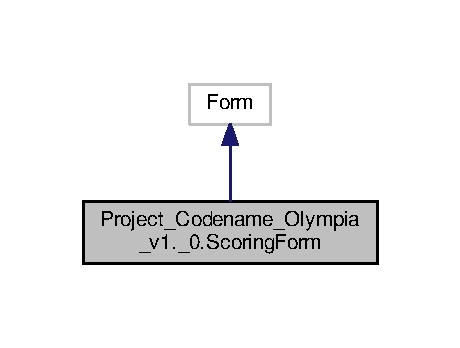
\includegraphics[width=241pt]{classProject__Codename__Olympia__v1_1_1__0_1_1ScoringForm__inherit__graph}
\end{center}
\end{figure}


Collaboration diagram for Project\+\_\+\+Codename\+\_\+\+Olympia\+\_\+v1.\+\_\+0.\+Scoring\+Form\+:\nopagebreak
\begin{figure}[H]
\begin{center}
\leavevmode
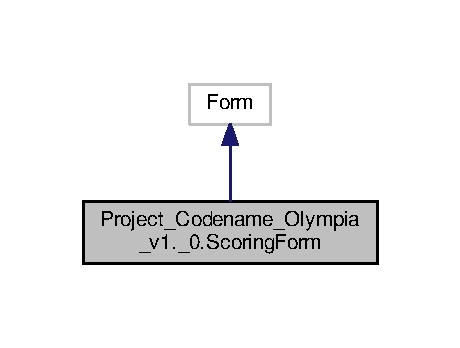
\includegraphics[width=243pt]{classProject__Codename__Olympia__v1_1_1__0_1_1ScoringForm__coll__graph}
\end{center}
\end{figure}
\subsection*{Public Member Functions}
\begin{DoxyCompactItemize}
\item 
\hyperlink{classProject__Codename__Olympia__v1_1_1__0_1_1ScoringForm_a4a85ebb20f6f24612e3d6509c901595b}{Scoring\+Form} ()
\end{DoxyCompactItemize}
\subsection*{Protected Member Functions}
\begin{DoxyCompactItemize}
\item 
override void \hyperlink{classProject__Codename__Olympia__v1_1_1__0_1_1ScoringForm_a6617b54014c935162ab2dd0746a3888e}{Dispose} (bool disposing)
\begin{DoxyCompactList}\small\item\em Clean up any resources being used. \end{DoxyCompactList}\end{DoxyCompactItemize}
\subsection*{Private Member Functions}
\begin{DoxyCompactItemize}
\item 
void \hyperlink{classProject__Codename__Olympia__v1_1_1__0_1_1ScoringForm_a6f80dfe3da06bba62c43b7b0b7444075}{Form5\+\_\+\+Load} (object sender, Event\+Args e)
\item 
void \hyperlink{classProject__Codename__Olympia__v1_1_1__0_1_1ScoringForm_aaa345dde4bac5b6a5503447bf199c453}{list\+Box1\+\_\+\+Selected\+Index\+Changed} (object sender, Event\+Args e)
\item 
void \hyperlink{classProject__Codename__Olympia__v1_1_1__0_1_1ScoringForm_a1abcd2e1c76528c880860eedf1f7214b}{button1\+\_\+\+Click} (object sender, Event\+Args e)
\item 
void \hyperlink{classProject__Codename__Olympia__v1_1_1__0_1_1ScoringForm_a514aa4c5e779c6a4ca849a42273a6c11}{data\+Grid\+View1\+\_\+\+Cell\+Content\+Click} (object sender, Data\+Grid\+View\+Cell\+Event\+Args e)
\item 
void \hyperlink{classProject__Codename__Olympia__v1_1_1__0_1_1ScoringForm_a355c176cd1e59eeb4017a97d727f93a2}{button2\+\_\+\+Click} (object sender, Event\+Args e)
\item 
void \hyperlink{classProject__Codename__Olympia__v1_1_1__0_1_1ScoringForm_a15a943f39dd97ecf0bdf0570bd93e9e7}{button3\+\_\+\+Click} (object sender, Event\+Args e)
\item 
void \hyperlink{classProject__Codename__Olympia__v1_1_1__0_1_1ScoringForm_ac0361aaff7cc21ee35c17d402a2d63cd}{Initialize\+Component} ()
\begin{DoxyCompactList}\small\item\em Required method for Designer support -\/ do not modify the contents of this method with the code editor. \end{DoxyCompactList}\end{DoxyCompactItemize}
\subsection*{Private Attributes}
\begin{DoxyCompactItemize}
\item 
string \hyperlink{classProject__Codename__Olympia__v1_1_1__0_1_1ScoringForm_a93760c23c8a04122d96f9ba29adc7f79}{Selected\+Event}
\item 
System.\+Component\+Model.\+I\+Container \hyperlink{classProject__Codename__Olympia__v1_1_1__0_1_1ScoringForm_a7a32c6e8e5131ea279dcfedc3166ffe4}{components} = null
\begin{DoxyCompactList}\small\item\em Required designer variable. \end{DoxyCompactList}\item 
System.\+Windows.\+Forms.\+Data\+Grid\+View \hyperlink{classProject__Codename__Olympia__v1_1_1__0_1_1ScoringForm_aa421e7b28ebbb430c6892a711b6f823b}{data\+Grid\+View1}
\item 
System.\+Windows.\+Forms.\+List\+Box \hyperlink{classProject__Codename__Olympia__v1_1_1__0_1_1ScoringForm_a72901fc5feff3003cdc038cfbf1d4bcc}{list\+Box1}
\item 
System.\+Windows.\+Forms.\+Button \hyperlink{classProject__Codename__Olympia__v1_1_1__0_1_1ScoringForm_ae9299ebbd6c5a116dfcb48b4838c2ba0}{button1}
\item 
System.\+Windows.\+Forms.\+Label \hyperlink{classProject__Codename__Olympia__v1_1_1__0_1_1ScoringForm_a102bf1793a3f3883100538f7ed8e9493}{label1}
\item 
System.\+Windows.\+Forms.\+Label \hyperlink{classProject__Codename__Olympia__v1_1_1__0_1_1ScoringForm_a5a9769bf47df100077650afed0afc1b3}{label2}
\item 
System.\+Windows.\+Forms.\+Label \hyperlink{classProject__Codename__Olympia__v1_1_1__0_1_1ScoringForm_a5862e2dce286250a07381afed0012f00}{label3}
\item 
System.\+Windows.\+Forms.\+Data\+Grid\+View\+Text\+Box\+Column \hyperlink{classProject__Codename__Olympia__v1_1_1__0_1_1ScoringForm_a908034221bf7665e924c4c393f868a84}{Place}
\item 
System.\+Windows.\+Forms.\+Button \hyperlink{classProject__Codename__Olympia__v1_1_1__0_1_1ScoringForm_a90bcb7c0e517fe0bbeacd47bc6351eaf}{button2}
\item 
System.\+Windows.\+Forms.\+Text\+Box \hyperlink{classProject__Codename__Olympia__v1_1_1__0_1_1ScoringForm_ab842136ba522120328485d1a0b7acff3}{text\+Box1}
\item 
System.\+Windows.\+Forms.\+Label \hyperlink{classProject__Codename__Olympia__v1_1_1__0_1_1ScoringForm_aff242897e95b72d1ad48c90b512f859d}{label4}
\item 
System.\+Windows.\+Forms.\+Text\+Box \hyperlink{classProject__Codename__Olympia__v1_1_1__0_1_1ScoringForm_af5a57b51e4c2c83c66418834b5ff226a}{text\+Box2}
\item 
System.\+Windows.\+Forms.\+Text\+Box \hyperlink{classProject__Codename__Olympia__v1_1_1__0_1_1ScoringForm_a437bf56ba4b2de0a2ec39375006419a1}{text\+Box3}
\item 
System.\+Windows.\+Forms.\+Text\+Box \hyperlink{classProject__Codename__Olympia__v1_1_1__0_1_1ScoringForm_ac1d0a0c98752fb75b0740414a9b2ec81}{text\+Box4}
\item 
System.\+Windows.\+Forms.\+Text\+Box \hyperlink{classProject__Codename__Olympia__v1_1_1__0_1_1ScoringForm_a2ab08e1a40ff604d53fec081a90dae04}{text\+Box5}
\item 
System.\+Windows.\+Forms.\+Text\+Box \hyperlink{classProject__Codename__Olympia__v1_1_1__0_1_1ScoringForm_a5c85e25caf9018cf7e83274c7df44729}{text\+Box6}
\item 
System.\+Windows.\+Forms.\+Text\+Box \hyperlink{classProject__Codename__Olympia__v1_1_1__0_1_1ScoringForm_a379e00e21671639e020eb2ff46a30eeb}{text\+Box7}
\item 
System.\+Windows.\+Forms.\+Text\+Box \hyperlink{classProject__Codename__Olympia__v1_1_1__0_1_1ScoringForm_a1937b608ccb900235fc4102b8704c83c}{text\+Box8}
\item 
System.\+Windows.\+Forms.\+Button \hyperlink{classProject__Codename__Olympia__v1_1_1__0_1_1ScoringForm_a7ac717cf762ee6f76d5cb56d64b3ed9c}{button3}
\item 
System.\+Windows.\+Forms.\+Label \hyperlink{classProject__Codename__Olympia__v1_1_1__0_1_1ScoringForm_a27b6461005d1b3dbaac8c9a9aed1708f}{label5}
\item 
System.\+Windows.\+Forms.\+Label \hyperlink{classProject__Codename__Olympia__v1_1_1__0_1_1ScoringForm_ab629e02b570ecaf21398f2e8fb342f15}{label6}
\item 
System.\+Windows.\+Forms.\+Label \hyperlink{classProject__Codename__Olympia__v1_1_1__0_1_1ScoringForm_afc5b612313aeaa61f418e9c5110df028}{label7}
\end{DoxyCompactItemize}


\subsection{Detailed Description}


Definition at line 15 of file Judge.\+cs.



\subsection{Constructor \& Destructor Documentation}
\mbox{\Hypertarget{classProject__Codename__Olympia__v1_1_1__0_1_1ScoringForm_a4a85ebb20f6f24612e3d6509c901595b}\label{classProject__Codename__Olympia__v1_1_1__0_1_1ScoringForm_a4a85ebb20f6f24612e3d6509c901595b}} 
\index{Project\+\_\+\+Codename\+\_\+\+Olympia\+\_\+v1\+::\+\_\+0\+::\+Scoring\+Form@{Project\+\_\+\+Codename\+\_\+\+Olympia\+\_\+v1\+::\+\_\+0\+::\+Scoring\+Form}!Scoring\+Form@{Scoring\+Form}}
\index{Scoring\+Form@{Scoring\+Form}!Project\+\_\+\+Codename\+\_\+\+Olympia\+\_\+v1\+::\+\_\+0\+::\+Scoring\+Form@{Project\+\_\+\+Codename\+\_\+\+Olympia\+\_\+v1\+::\+\_\+0\+::\+Scoring\+Form}}
\subsubsection{\texorpdfstring{Scoring\+Form()}{ScoringForm()}}
{\footnotesize\ttfamily Project\+\_\+\+Codename\+\_\+\+Olympia\+\_\+v1.\+\_\+0.\+Scoring\+Form.\+Scoring\+Form (\begin{DoxyParamCaption}{ }\end{DoxyParamCaption})\hspace{0.3cm}{\ttfamily [inline]}}



Definition at line 18 of file Judge.\+cs.



\subsection{Member Function Documentation}
\mbox{\Hypertarget{classProject__Codename__Olympia__v1_1_1__0_1_1ScoringForm_a1abcd2e1c76528c880860eedf1f7214b}\label{classProject__Codename__Olympia__v1_1_1__0_1_1ScoringForm_a1abcd2e1c76528c880860eedf1f7214b}} 
\index{Project\+\_\+\+Codename\+\_\+\+Olympia\+\_\+v1\+::\+\_\+0\+::\+Scoring\+Form@{Project\+\_\+\+Codename\+\_\+\+Olympia\+\_\+v1\+::\+\_\+0\+::\+Scoring\+Form}!button1\+\_\+\+Click@{button1\+\_\+\+Click}}
\index{button1\+\_\+\+Click@{button1\+\_\+\+Click}!Project\+\_\+\+Codename\+\_\+\+Olympia\+\_\+v1\+::\+\_\+0\+::\+Scoring\+Form@{Project\+\_\+\+Codename\+\_\+\+Olympia\+\_\+v1\+::\+\_\+0\+::\+Scoring\+Form}}
\subsubsection{\texorpdfstring{button1\+\_\+\+Click()}{button1\_Click()}}
{\footnotesize\ttfamily void Project\+\_\+\+Codename\+\_\+\+Olympia\+\_\+v1.\+\_\+0.\+Scoring\+Form.\+button1\+\_\+\+Click (\begin{DoxyParamCaption}\item[{object}]{sender,  }\item[{Event\+Args}]{e }\end{DoxyParamCaption})\hspace{0.3cm}{\ttfamily [inline]}, {\ttfamily [private]}}



Definition at line 72 of file Judge.\+cs.

\mbox{\Hypertarget{classProject__Codename__Olympia__v1_1_1__0_1_1ScoringForm_a355c176cd1e59eeb4017a97d727f93a2}\label{classProject__Codename__Olympia__v1_1_1__0_1_1ScoringForm_a355c176cd1e59eeb4017a97d727f93a2}} 
\index{Project\+\_\+\+Codename\+\_\+\+Olympia\+\_\+v1\+::\+\_\+0\+::\+Scoring\+Form@{Project\+\_\+\+Codename\+\_\+\+Olympia\+\_\+v1\+::\+\_\+0\+::\+Scoring\+Form}!button2\+\_\+\+Click@{button2\+\_\+\+Click}}
\index{button2\+\_\+\+Click@{button2\+\_\+\+Click}!Project\+\_\+\+Codename\+\_\+\+Olympia\+\_\+v1\+::\+\_\+0\+::\+Scoring\+Form@{Project\+\_\+\+Codename\+\_\+\+Olympia\+\_\+v1\+::\+\_\+0\+::\+Scoring\+Form}}
\subsubsection{\texorpdfstring{button2\+\_\+\+Click()}{button2\_Click()}}
{\footnotesize\ttfamily void Project\+\_\+\+Codename\+\_\+\+Olympia\+\_\+v1.\+\_\+0.\+Scoring\+Form.\+button2\+\_\+\+Click (\begin{DoxyParamCaption}\item[{object}]{sender,  }\item[{Event\+Args}]{e }\end{DoxyParamCaption})\hspace{0.3cm}{\ttfamily [inline]}, {\ttfamily [private]}}



Definition at line 612 of file Judge.\+cs.

\mbox{\Hypertarget{classProject__Codename__Olympia__v1_1_1__0_1_1ScoringForm_a15a943f39dd97ecf0bdf0570bd93e9e7}\label{classProject__Codename__Olympia__v1_1_1__0_1_1ScoringForm_a15a943f39dd97ecf0bdf0570bd93e9e7}} 
\index{Project\+\_\+\+Codename\+\_\+\+Olympia\+\_\+v1\+::\+\_\+0\+::\+Scoring\+Form@{Project\+\_\+\+Codename\+\_\+\+Olympia\+\_\+v1\+::\+\_\+0\+::\+Scoring\+Form}!button3\+\_\+\+Click@{button3\+\_\+\+Click}}
\index{button3\+\_\+\+Click@{button3\+\_\+\+Click}!Project\+\_\+\+Codename\+\_\+\+Olympia\+\_\+v1\+::\+\_\+0\+::\+Scoring\+Form@{Project\+\_\+\+Codename\+\_\+\+Olympia\+\_\+v1\+::\+\_\+0\+::\+Scoring\+Form}}
\subsubsection{\texorpdfstring{button3\+\_\+\+Click()}{button3\_Click()}}
{\footnotesize\ttfamily void Project\+\_\+\+Codename\+\_\+\+Olympia\+\_\+v1.\+\_\+0.\+Scoring\+Form.\+button3\+\_\+\+Click (\begin{DoxyParamCaption}\item[{object}]{sender,  }\item[{Event\+Args}]{e }\end{DoxyParamCaption})\hspace{0.3cm}{\ttfamily [inline]}, {\ttfamily [private]}}



Definition at line 649 of file Judge.\+cs.

\mbox{\Hypertarget{classProject__Codename__Olympia__v1_1_1__0_1_1ScoringForm_a514aa4c5e779c6a4ca849a42273a6c11}\label{classProject__Codename__Olympia__v1_1_1__0_1_1ScoringForm_a514aa4c5e779c6a4ca849a42273a6c11}} 
\index{Project\+\_\+\+Codename\+\_\+\+Olympia\+\_\+v1\+::\+\_\+0\+::\+Scoring\+Form@{Project\+\_\+\+Codename\+\_\+\+Olympia\+\_\+v1\+::\+\_\+0\+::\+Scoring\+Form}!data\+Grid\+View1\+\_\+\+Cell\+Content\+Click@{data\+Grid\+View1\+\_\+\+Cell\+Content\+Click}}
\index{data\+Grid\+View1\+\_\+\+Cell\+Content\+Click@{data\+Grid\+View1\+\_\+\+Cell\+Content\+Click}!Project\+\_\+\+Codename\+\_\+\+Olympia\+\_\+v1\+::\+\_\+0\+::\+Scoring\+Form@{Project\+\_\+\+Codename\+\_\+\+Olympia\+\_\+v1\+::\+\_\+0\+::\+Scoring\+Form}}
\subsubsection{\texorpdfstring{data\+Grid\+View1\+\_\+\+Cell\+Content\+Click()}{dataGridView1\_CellContentClick()}}
{\footnotesize\ttfamily void Project\+\_\+\+Codename\+\_\+\+Olympia\+\_\+v1.\+\_\+0.\+Scoring\+Form.\+data\+Grid\+View1\+\_\+\+Cell\+Content\+Click (\begin{DoxyParamCaption}\item[{object}]{sender,  }\item[{Data\+Grid\+View\+Cell\+Event\+Args}]{e }\end{DoxyParamCaption})\hspace{0.3cm}{\ttfamily [inline]}, {\ttfamily [private]}}



Definition at line 607 of file Judge.\+cs.

\mbox{\Hypertarget{classProject__Codename__Olympia__v1_1_1__0_1_1ScoringForm_a6617b54014c935162ab2dd0746a3888e}\label{classProject__Codename__Olympia__v1_1_1__0_1_1ScoringForm_a6617b54014c935162ab2dd0746a3888e}} 
\index{Project\+\_\+\+Codename\+\_\+\+Olympia\+\_\+v1\+::\+\_\+0\+::\+Scoring\+Form@{Project\+\_\+\+Codename\+\_\+\+Olympia\+\_\+v1\+::\+\_\+0\+::\+Scoring\+Form}!Dispose@{Dispose}}
\index{Dispose@{Dispose}!Project\+\_\+\+Codename\+\_\+\+Olympia\+\_\+v1\+::\+\_\+0\+::\+Scoring\+Form@{Project\+\_\+\+Codename\+\_\+\+Olympia\+\_\+v1\+::\+\_\+0\+::\+Scoring\+Form}}
\subsubsection{\texorpdfstring{Dispose()}{Dispose()}}
{\footnotesize\ttfamily override void Project\+\_\+\+Codename\+\_\+\+Olympia\+\_\+v1.\+\_\+0.\+Scoring\+Form.\+Dispose (\begin{DoxyParamCaption}\item[{bool}]{disposing }\end{DoxyParamCaption})\hspace{0.3cm}{\ttfamily [inline]}, {\ttfamily [protected]}}



Clean up any resources being used. 


\begin{DoxyParams}{Parameters}
{\em disposing} & true if managed resources should be disposed; otherwise, false.\\
\hline
\end{DoxyParams}


Definition at line 14 of file Judge.\+Designer.\+cs.

\mbox{\Hypertarget{classProject__Codename__Olympia__v1_1_1__0_1_1ScoringForm_a6f80dfe3da06bba62c43b7b0b7444075}\label{classProject__Codename__Olympia__v1_1_1__0_1_1ScoringForm_a6f80dfe3da06bba62c43b7b0b7444075}} 
\index{Project\+\_\+\+Codename\+\_\+\+Olympia\+\_\+v1\+::\+\_\+0\+::\+Scoring\+Form@{Project\+\_\+\+Codename\+\_\+\+Olympia\+\_\+v1\+::\+\_\+0\+::\+Scoring\+Form}!Form5\+\_\+\+Load@{Form5\+\_\+\+Load}}
\index{Form5\+\_\+\+Load@{Form5\+\_\+\+Load}!Project\+\_\+\+Codename\+\_\+\+Olympia\+\_\+v1\+::\+\_\+0\+::\+Scoring\+Form@{Project\+\_\+\+Codename\+\_\+\+Olympia\+\_\+v1\+::\+\_\+0\+::\+Scoring\+Form}}
\subsubsection{\texorpdfstring{Form5\+\_\+\+Load()}{Form5\_Load()}}
{\footnotesize\ttfamily void Project\+\_\+\+Codename\+\_\+\+Olympia\+\_\+v1.\+\_\+0.\+Scoring\+Form.\+Form5\+\_\+\+Load (\begin{DoxyParamCaption}\item[{object}]{sender,  }\item[{Event\+Args}]{e }\end{DoxyParamCaption})\hspace{0.3cm}{\ttfamily [inline]}, {\ttfamily [private]}}



Definition at line 23 of file Judge.\+cs.

\mbox{\Hypertarget{classProject__Codename__Olympia__v1_1_1__0_1_1ScoringForm_ac0361aaff7cc21ee35c17d402a2d63cd}\label{classProject__Codename__Olympia__v1_1_1__0_1_1ScoringForm_ac0361aaff7cc21ee35c17d402a2d63cd}} 
\index{Project\+\_\+\+Codename\+\_\+\+Olympia\+\_\+v1\+::\+\_\+0\+::\+Scoring\+Form@{Project\+\_\+\+Codename\+\_\+\+Olympia\+\_\+v1\+::\+\_\+0\+::\+Scoring\+Form}!Initialize\+Component@{Initialize\+Component}}
\index{Initialize\+Component@{Initialize\+Component}!Project\+\_\+\+Codename\+\_\+\+Olympia\+\_\+v1\+::\+\_\+0\+::\+Scoring\+Form@{Project\+\_\+\+Codename\+\_\+\+Olympia\+\_\+v1\+::\+\_\+0\+::\+Scoring\+Form}}
\subsubsection{\texorpdfstring{Initialize\+Component()}{InitializeComponent()}}
{\footnotesize\ttfamily void Project\+\_\+\+Codename\+\_\+\+Olympia\+\_\+v1.\+\_\+0.\+Scoring\+Form.\+Initialize\+Component (\begin{DoxyParamCaption}{ }\end{DoxyParamCaption})\hspace{0.3cm}{\ttfamily [inline]}, {\ttfamily [private]}}



Required method for Designer support -\/ do not modify the contents of this method with the code editor. 



Definition at line 29 of file Judge.\+Designer.\+cs.

\mbox{\Hypertarget{classProject__Codename__Olympia__v1_1_1__0_1_1ScoringForm_aaa345dde4bac5b6a5503447bf199c453}\label{classProject__Codename__Olympia__v1_1_1__0_1_1ScoringForm_aaa345dde4bac5b6a5503447bf199c453}} 
\index{Project\+\_\+\+Codename\+\_\+\+Olympia\+\_\+v1\+::\+\_\+0\+::\+Scoring\+Form@{Project\+\_\+\+Codename\+\_\+\+Olympia\+\_\+v1\+::\+\_\+0\+::\+Scoring\+Form}!list\+Box1\+\_\+\+Selected\+Index\+Changed@{list\+Box1\+\_\+\+Selected\+Index\+Changed}}
\index{list\+Box1\+\_\+\+Selected\+Index\+Changed@{list\+Box1\+\_\+\+Selected\+Index\+Changed}!Project\+\_\+\+Codename\+\_\+\+Olympia\+\_\+v1\+::\+\_\+0\+::\+Scoring\+Form@{Project\+\_\+\+Codename\+\_\+\+Olympia\+\_\+v1\+::\+\_\+0\+::\+Scoring\+Form}}
\subsubsection{\texorpdfstring{list\+Box1\+\_\+\+Selected\+Index\+Changed()}{listBox1\_SelectedIndexChanged()}}
{\footnotesize\ttfamily void Project\+\_\+\+Codename\+\_\+\+Olympia\+\_\+v1.\+\_\+0.\+Scoring\+Form.\+list\+Box1\+\_\+\+Selected\+Index\+Changed (\begin{DoxyParamCaption}\item[{object}]{sender,  }\item[{Event\+Args}]{e }\end{DoxyParamCaption})\hspace{0.3cm}{\ttfamily [inline]}, {\ttfamily [private]}}



Definition at line 67 of file Judge.\+cs.



\subsection{Member Data Documentation}
\mbox{\Hypertarget{classProject__Codename__Olympia__v1_1_1__0_1_1ScoringForm_ae9299ebbd6c5a116dfcb48b4838c2ba0}\label{classProject__Codename__Olympia__v1_1_1__0_1_1ScoringForm_ae9299ebbd6c5a116dfcb48b4838c2ba0}} 
\index{Project\+\_\+\+Codename\+\_\+\+Olympia\+\_\+v1\+::\+\_\+0\+::\+Scoring\+Form@{Project\+\_\+\+Codename\+\_\+\+Olympia\+\_\+v1\+::\+\_\+0\+::\+Scoring\+Form}!button1@{button1}}
\index{button1@{button1}!Project\+\_\+\+Codename\+\_\+\+Olympia\+\_\+v1\+::\+\_\+0\+::\+Scoring\+Form@{Project\+\_\+\+Codename\+\_\+\+Olympia\+\_\+v1\+::\+\_\+0\+::\+Scoring\+Form}}
\subsubsection{\texorpdfstring{button1}{button1}}
{\footnotesize\ttfamily System.\+Windows.\+Forms.\+Button Project\+\_\+\+Codename\+\_\+\+Olympia\+\_\+v1.\+\_\+0.\+Scoring\+Form.\+button1\hspace{0.3cm}{\ttfamily [private]}}



Definition at line 286 of file Judge.\+Designer.\+cs.

\mbox{\Hypertarget{classProject__Codename__Olympia__v1_1_1__0_1_1ScoringForm_a90bcb7c0e517fe0bbeacd47bc6351eaf}\label{classProject__Codename__Olympia__v1_1_1__0_1_1ScoringForm_a90bcb7c0e517fe0bbeacd47bc6351eaf}} 
\index{Project\+\_\+\+Codename\+\_\+\+Olympia\+\_\+v1\+::\+\_\+0\+::\+Scoring\+Form@{Project\+\_\+\+Codename\+\_\+\+Olympia\+\_\+v1\+::\+\_\+0\+::\+Scoring\+Form}!button2@{button2}}
\index{button2@{button2}!Project\+\_\+\+Codename\+\_\+\+Olympia\+\_\+v1\+::\+\_\+0\+::\+Scoring\+Form@{Project\+\_\+\+Codename\+\_\+\+Olympia\+\_\+v1\+::\+\_\+0\+::\+Scoring\+Form}}
\subsubsection{\texorpdfstring{button2}{button2}}
{\footnotesize\ttfamily System.\+Windows.\+Forms.\+Button Project\+\_\+\+Codename\+\_\+\+Olympia\+\_\+v1.\+\_\+0.\+Scoring\+Form.\+button2\hspace{0.3cm}{\ttfamily [private]}}



Definition at line 291 of file Judge.\+Designer.\+cs.

\mbox{\Hypertarget{classProject__Codename__Olympia__v1_1_1__0_1_1ScoringForm_a7ac717cf762ee6f76d5cb56d64b3ed9c}\label{classProject__Codename__Olympia__v1_1_1__0_1_1ScoringForm_a7ac717cf762ee6f76d5cb56d64b3ed9c}} 
\index{Project\+\_\+\+Codename\+\_\+\+Olympia\+\_\+v1\+::\+\_\+0\+::\+Scoring\+Form@{Project\+\_\+\+Codename\+\_\+\+Olympia\+\_\+v1\+::\+\_\+0\+::\+Scoring\+Form}!button3@{button3}}
\index{button3@{button3}!Project\+\_\+\+Codename\+\_\+\+Olympia\+\_\+v1\+::\+\_\+0\+::\+Scoring\+Form@{Project\+\_\+\+Codename\+\_\+\+Olympia\+\_\+v1\+::\+\_\+0\+::\+Scoring\+Form}}
\subsubsection{\texorpdfstring{button3}{button3}}
{\footnotesize\ttfamily System.\+Windows.\+Forms.\+Button Project\+\_\+\+Codename\+\_\+\+Olympia\+\_\+v1.\+\_\+0.\+Scoring\+Form.\+button3\hspace{0.3cm}{\ttfamily [private]}}



Definition at line 301 of file Judge.\+Designer.\+cs.

\mbox{\Hypertarget{classProject__Codename__Olympia__v1_1_1__0_1_1ScoringForm_a7a32c6e8e5131ea279dcfedc3166ffe4}\label{classProject__Codename__Olympia__v1_1_1__0_1_1ScoringForm_a7a32c6e8e5131ea279dcfedc3166ffe4}} 
\index{Project\+\_\+\+Codename\+\_\+\+Olympia\+\_\+v1\+::\+\_\+0\+::\+Scoring\+Form@{Project\+\_\+\+Codename\+\_\+\+Olympia\+\_\+v1\+::\+\_\+0\+::\+Scoring\+Form}!components@{components}}
\index{components@{components}!Project\+\_\+\+Codename\+\_\+\+Olympia\+\_\+v1\+::\+\_\+0\+::\+Scoring\+Form@{Project\+\_\+\+Codename\+\_\+\+Olympia\+\_\+v1\+::\+\_\+0\+::\+Scoring\+Form}}
\subsubsection{\texorpdfstring{components}{components}}
{\footnotesize\ttfamily System.\+Component\+Model.\+I\+Container Project\+\_\+\+Codename\+\_\+\+Olympia\+\_\+v1.\+\_\+0.\+Scoring\+Form.\+components = null\hspace{0.3cm}{\ttfamily [private]}}



Required designer variable. 



Definition at line 8 of file Judge.\+Designer.\+cs.

\mbox{\Hypertarget{classProject__Codename__Olympia__v1_1_1__0_1_1ScoringForm_aa421e7b28ebbb430c6892a711b6f823b}\label{classProject__Codename__Olympia__v1_1_1__0_1_1ScoringForm_aa421e7b28ebbb430c6892a711b6f823b}} 
\index{Project\+\_\+\+Codename\+\_\+\+Olympia\+\_\+v1\+::\+\_\+0\+::\+Scoring\+Form@{Project\+\_\+\+Codename\+\_\+\+Olympia\+\_\+v1\+::\+\_\+0\+::\+Scoring\+Form}!data\+Grid\+View1@{data\+Grid\+View1}}
\index{data\+Grid\+View1@{data\+Grid\+View1}!Project\+\_\+\+Codename\+\_\+\+Olympia\+\_\+v1\+::\+\_\+0\+::\+Scoring\+Form@{Project\+\_\+\+Codename\+\_\+\+Olympia\+\_\+v1\+::\+\_\+0\+::\+Scoring\+Form}}
\subsubsection{\texorpdfstring{data\+Grid\+View1}{dataGridView1}}
{\footnotesize\ttfamily System.\+Windows.\+Forms.\+Data\+Grid\+View Project\+\_\+\+Codename\+\_\+\+Olympia\+\_\+v1.\+\_\+0.\+Scoring\+Form.\+data\+Grid\+View1\hspace{0.3cm}{\ttfamily [private]}}



Definition at line 284 of file Judge.\+Designer.\+cs.

\mbox{\Hypertarget{classProject__Codename__Olympia__v1_1_1__0_1_1ScoringForm_a102bf1793a3f3883100538f7ed8e9493}\label{classProject__Codename__Olympia__v1_1_1__0_1_1ScoringForm_a102bf1793a3f3883100538f7ed8e9493}} 
\index{Project\+\_\+\+Codename\+\_\+\+Olympia\+\_\+v1\+::\+\_\+0\+::\+Scoring\+Form@{Project\+\_\+\+Codename\+\_\+\+Olympia\+\_\+v1\+::\+\_\+0\+::\+Scoring\+Form}!label1@{label1}}
\index{label1@{label1}!Project\+\_\+\+Codename\+\_\+\+Olympia\+\_\+v1\+::\+\_\+0\+::\+Scoring\+Form@{Project\+\_\+\+Codename\+\_\+\+Olympia\+\_\+v1\+::\+\_\+0\+::\+Scoring\+Form}}
\subsubsection{\texorpdfstring{label1}{label1}}
{\footnotesize\ttfamily System.\+Windows.\+Forms.\+Label Project\+\_\+\+Codename\+\_\+\+Olympia\+\_\+v1.\+\_\+0.\+Scoring\+Form.\+label1\hspace{0.3cm}{\ttfamily [private]}}



Definition at line 287 of file Judge.\+Designer.\+cs.

\mbox{\Hypertarget{classProject__Codename__Olympia__v1_1_1__0_1_1ScoringForm_a5a9769bf47df100077650afed0afc1b3}\label{classProject__Codename__Olympia__v1_1_1__0_1_1ScoringForm_a5a9769bf47df100077650afed0afc1b3}} 
\index{Project\+\_\+\+Codename\+\_\+\+Olympia\+\_\+v1\+::\+\_\+0\+::\+Scoring\+Form@{Project\+\_\+\+Codename\+\_\+\+Olympia\+\_\+v1\+::\+\_\+0\+::\+Scoring\+Form}!label2@{label2}}
\index{label2@{label2}!Project\+\_\+\+Codename\+\_\+\+Olympia\+\_\+v1\+::\+\_\+0\+::\+Scoring\+Form@{Project\+\_\+\+Codename\+\_\+\+Olympia\+\_\+v1\+::\+\_\+0\+::\+Scoring\+Form}}
\subsubsection{\texorpdfstring{label2}{label2}}
{\footnotesize\ttfamily System.\+Windows.\+Forms.\+Label Project\+\_\+\+Codename\+\_\+\+Olympia\+\_\+v1.\+\_\+0.\+Scoring\+Form.\+label2\hspace{0.3cm}{\ttfamily [private]}}



Definition at line 288 of file Judge.\+Designer.\+cs.

\mbox{\Hypertarget{classProject__Codename__Olympia__v1_1_1__0_1_1ScoringForm_a5862e2dce286250a07381afed0012f00}\label{classProject__Codename__Olympia__v1_1_1__0_1_1ScoringForm_a5862e2dce286250a07381afed0012f00}} 
\index{Project\+\_\+\+Codename\+\_\+\+Olympia\+\_\+v1\+::\+\_\+0\+::\+Scoring\+Form@{Project\+\_\+\+Codename\+\_\+\+Olympia\+\_\+v1\+::\+\_\+0\+::\+Scoring\+Form}!label3@{label3}}
\index{label3@{label3}!Project\+\_\+\+Codename\+\_\+\+Olympia\+\_\+v1\+::\+\_\+0\+::\+Scoring\+Form@{Project\+\_\+\+Codename\+\_\+\+Olympia\+\_\+v1\+::\+\_\+0\+::\+Scoring\+Form}}
\subsubsection{\texorpdfstring{label3}{label3}}
{\footnotesize\ttfamily System.\+Windows.\+Forms.\+Label Project\+\_\+\+Codename\+\_\+\+Olympia\+\_\+v1.\+\_\+0.\+Scoring\+Form.\+label3\hspace{0.3cm}{\ttfamily [private]}}



Definition at line 289 of file Judge.\+Designer.\+cs.

\mbox{\Hypertarget{classProject__Codename__Olympia__v1_1_1__0_1_1ScoringForm_aff242897e95b72d1ad48c90b512f859d}\label{classProject__Codename__Olympia__v1_1_1__0_1_1ScoringForm_aff242897e95b72d1ad48c90b512f859d}} 
\index{Project\+\_\+\+Codename\+\_\+\+Olympia\+\_\+v1\+::\+\_\+0\+::\+Scoring\+Form@{Project\+\_\+\+Codename\+\_\+\+Olympia\+\_\+v1\+::\+\_\+0\+::\+Scoring\+Form}!label4@{label4}}
\index{label4@{label4}!Project\+\_\+\+Codename\+\_\+\+Olympia\+\_\+v1\+::\+\_\+0\+::\+Scoring\+Form@{Project\+\_\+\+Codename\+\_\+\+Olympia\+\_\+v1\+::\+\_\+0\+::\+Scoring\+Form}}
\subsubsection{\texorpdfstring{label4}{label4}}
{\footnotesize\ttfamily System.\+Windows.\+Forms.\+Label Project\+\_\+\+Codename\+\_\+\+Olympia\+\_\+v1.\+\_\+0.\+Scoring\+Form.\+label4\hspace{0.3cm}{\ttfamily [private]}}



Definition at line 293 of file Judge.\+Designer.\+cs.

\mbox{\Hypertarget{classProject__Codename__Olympia__v1_1_1__0_1_1ScoringForm_a27b6461005d1b3dbaac8c9a9aed1708f}\label{classProject__Codename__Olympia__v1_1_1__0_1_1ScoringForm_a27b6461005d1b3dbaac8c9a9aed1708f}} 
\index{Project\+\_\+\+Codename\+\_\+\+Olympia\+\_\+v1\+::\+\_\+0\+::\+Scoring\+Form@{Project\+\_\+\+Codename\+\_\+\+Olympia\+\_\+v1\+::\+\_\+0\+::\+Scoring\+Form}!label5@{label5}}
\index{label5@{label5}!Project\+\_\+\+Codename\+\_\+\+Olympia\+\_\+v1\+::\+\_\+0\+::\+Scoring\+Form@{Project\+\_\+\+Codename\+\_\+\+Olympia\+\_\+v1\+::\+\_\+0\+::\+Scoring\+Form}}
\subsubsection{\texorpdfstring{label5}{label5}}
{\footnotesize\ttfamily System.\+Windows.\+Forms.\+Label Project\+\_\+\+Codename\+\_\+\+Olympia\+\_\+v1.\+\_\+0.\+Scoring\+Form.\+label5\hspace{0.3cm}{\ttfamily [private]}}



Definition at line 302 of file Judge.\+Designer.\+cs.

\mbox{\Hypertarget{classProject__Codename__Olympia__v1_1_1__0_1_1ScoringForm_ab629e02b570ecaf21398f2e8fb342f15}\label{classProject__Codename__Olympia__v1_1_1__0_1_1ScoringForm_ab629e02b570ecaf21398f2e8fb342f15}} 
\index{Project\+\_\+\+Codename\+\_\+\+Olympia\+\_\+v1\+::\+\_\+0\+::\+Scoring\+Form@{Project\+\_\+\+Codename\+\_\+\+Olympia\+\_\+v1\+::\+\_\+0\+::\+Scoring\+Form}!label6@{label6}}
\index{label6@{label6}!Project\+\_\+\+Codename\+\_\+\+Olympia\+\_\+v1\+::\+\_\+0\+::\+Scoring\+Form@{Project\+\_\+\+Codename\+\_\+\+Olympia\+\_\+v1\+::\+\_\+0\+::\+Scoring\+Form}}
\subsubsection{\texorpdfstring{label6}{label6}}
{\footnotesize\ttfamily System.\+Windows.\+Forms.\+Label Project\+\_\+\+Codename\+\_\+\+Olympia\+\_\+v1.\+\_\+0.\+Scoring\+Form.\+label6\hspace{0.3cm}{\ttfamily [private]}}



Definition at line 303 of file Judge.\+Designer.\+cs.

\mbox{\Hypertarget{classProject__Codename__Olympia__v1_1_1__0_1_1ScoringForm_afc5b612313aeaa61f418e9c5110df028}\label{classProject__Codename__Olympia__v1_1_1__0_1_1ScoringForm_afc5b612313aeaa61f418e9c5110df028}} 
\index{Project\+\_\+\+Codename\+\_\+\+Olympia\+\_\+v1\+::\+\_\+0\+::\+Scoring\+Form@{Project\+\_\+\+Codename\+\_\+\+Olympia\+\_\+v1\+::\+\_\+0\+::\+Scoring\+Form}!label7@{label7}}
\index{label7@{label7}!Project\+\_\+\+Codename\+\_\+\+Olympia\+\_\+v1\+::\+\_\+0\+::\+Scoring\+Form@{Project\+\_\+\+Codename\+\_\+\+Olympia\+\_\+v1\+::\+\_\+0\+::\+Scoring\+Form}}
\subsubsection{\texorpdfstring{label7}{label7}}
{\footnotesize\ttfamily System.\+Windows.\+Forms.\+Label Project\+\_\+\+Codename\+\_\+\+Olympia\+\_\+v1.\+\_\+0.\+Scoring\+Form.\+label7\hspace{0.3cm}{\ttfamily [private]}}



Definition at line 304 of file Judge.\+Designer.\+cs.

\mbox{\Hypertarget{classProject__Codename__Olympia__v1_1_1__0_1_1ScoringForm_a72901fc5feff3003cdc038cfbf1d4bcc}\label{classProject__Codename__Olympia__v1_1_1__0_1_1ScoringForm_a72901fc5feff3003cdc038cfbf1d4bcc}} 
\index{Project\+\_\+\+Codename\+\_\+\+Olympia\+\_\+v1\+::\+\_\+0\+::\+Scoring\+Form@{Project\+\_\+\+Codename\+\_\+\+Olympia\+\_\+v1\+::\+\_\+0\+::\+Scoring\+Form}!list\+Box1@{list\+Box1}}
\index{list\+Box1@{list\+Box1}!Project\+\_\+\+Codename\+\_\+\+Olympia\+\_\+v1\+::\+\_\+0\+::\+Scoring\+Form@{Project\+\_\+\+Codename\+\_\+\+Olympia\+\_\+v1\+::\+\_\+0\+::\+Scoring\+Form}}
\subsubsection{\texorpdfstring{list\+Box1}{listBox1}}
{\footnotesize\ttfamily System.\+Windows.\+Forms.\+List\+Box Project\+\_\+\+Codename\+\_\+\+Olympia\+\_\+v1.\+\_\+0.\+Scoring\+Form.\+list\+Box1\hspace{0.3cm}{\ttfamily [private]}}



Definition at line 285 of file Judge.\+Designer.\+cs.

\mbox{\Hypertarget{classProject__Codename__Olympia__v1_1_1__0_1_1ScoringForm_a908034221bf7665e924c4c393f868a84}\label{classProject__Codename__Olympia__v1_1_1__0_1_1ScoringForm_a908034221bf7665e924c4c393f868a84}} 
\index{Project\+\_\+\+Codename\+\_\+\+Olympia\+\_\+v1\+::\+\_\+0\+::\+Scoring\+Form@{Project\+\_\+\+Codename\+\_\+\+Olympia\+\_\+v1\+::\+\_\+0\+::\+Scoring\+Form}!Place@{Place}}
\index{Place@{Place}!Project\+\_\+\+Codename\+\_\+\+Olympia\+\_\+v1\+::\+\_\+0\+::\+Scoring\+Form@{Project\+\_\+\+Codename\+\_\+\+Olympia\+\_\+v1\+::\+\_\+0\+::\+Scoring\+Form}}
\subsubsection{\texorpdfstring{Place}{Place}}
{\footnotesize\ttfamily System.\+Windows.\+Forms.\+Data\+Grid\+View\+Text\+Box\+Column Project\+\_\+\+Codename\+\_\+\+Olympia\+\_\+v1.\+\_\+0.\+Scoring\+Form.\+Place\hspace{0.3cm}{\ttfamily [private]}}



Definition at line 290 of file Judge.\+Designer.\+cs.

\mbox{\Hypertarget{classProject__Codename__Olympia__v1_1_1__0_1_1ScoringForm_a93760c23c8a04122d96f9ba29adc7f79}\label{classProject__Codename__Olympia__v1_1_1__0_1_1ScoringForm_a93760c23c8a04122d96f9ba29adc7f79}} 
\index{Project\+\_\+\+Codename\+\_\+\+Olympia\+\_\+v1\+::\+\_\+0\+::\+Scoring\+Form@{Project\+\_\+\+Codename\+\_\+\+Olympia\+\_\+v1\+::\+\_\+0\+::\+Scoring\+Form}!Selected\+Event@{Selected\+Event}}
\index{Selected\+Event@{Selected\+Event}!Project\+\_\+\+Codename\+\_\+\+Olympia\+\_\+v1\+::\+\_\+0\+::\+Scoring\+Form@{Project\+\_\+\+Codename\+\_\+\+Olympia\+\_\+v1\+::\+\_\+0\+::\+Scoring\+Form}}
\subsubsection{\texorpdfstring{Selected\+Event}{SelectedEvent}}
{\footnotesize\ttfamily string Project\+\_\+\+Codename\+\_\+\+Olympia\+\_\+v1.\+\_\+0.\+Scoring\+Form.\+Selected\+Event\hspace{0.3cm}{\ttfamily [private]}}



Definition at line 17 of file Judge.\+cs.

\mbox{\Hypertarget{classProject__Codename__Olympia__v1_1_1__0_1_1ScoringForm_ab842136ba522120328485d1a0b7acff3}\label{classProject__Codename__Olympia__v1_1_1__0_1_1ScoringForm_ab842136ba522120328485d1a0b7acff3}} 
\index{Project\+\_\+\+Codename\+\_\+\+Olympia\+\_\+v1\+::\+\_\+0\+::\+Scoring\+Form@{Project\+\_\+\+Codename\+\_\+\+Olympia\+\_\+v1\+::\+\_\+0\+::\+Scoring\+Form}!text\+Box1@{text\+Box1}}
\index{text\+Box1@{text\+Box1}!Project\+\_\+\+Codename\+\_\+\+Olympia\+\_\+v1\+::\+\_\+0\+::\+Scoring\+Form@{Project\+\_\+\+Codename\+\_\+\+Olympia\+\_\+v1\+::\+\_\+0\+::\+Scoring\+Form}}
\subsubsection{\texorpdfstring{text\+Box1}{textBox1}}
{\footnotesize\ttfamily System.\+Windows.\+Forms.\+Text\+Box Project\+\_\+\+Codename\+\_\+\+Olympia\+\_\+v1.\+\_\+0.\+Scoring\+Form.\+text\+Box1\hspace{0.3cm}{\ttfamily [private]}}



Definition at line 292 of file Judge.\+Designer.\+cs.

\mbox{\Hypertarget{classProject__Codename__Olympia__v1_1_1__0_1_1ScoringForm_af5a57b51e4c2c83c66418834b5ff226a}\label{classProject__Codename__Olympia__v1_1_1__0_1_1ScoringForm_af5a57b51e4c2c83c66418834b5ff226a}} 
\index{Project\+\_\+\+Codename\+\_\+\+Olympia\+\_\+v1\+::\+\_\+0\+::\+Scoring\+Form@{Project\+\_\+\+Codename\+\_\+\+Olympia\+\_\+v1\+::\+\_\+0\+::\+Scoring\+Form}!text\+Box2@{text\+Box2}}
\index{text\+Box2@{text\+Box2}!Project\+\_\+\+Codename\+\_\+\+Olympia\+\_\+v1\+::\+\_\+0\+::\+Scoring\+Form@{Project\+\_\+\+Codename\+\_\+\+Olympia\+\_\+v1\+::\+\_\+0\+::\+Scoring\+Form}}
\subsubsection{\texorpdfstring{text\+Box2}{textBox2}}
{\footnotesize\ttfamily System.\+Windows.\+Forms.\+Text\+Box Project\+\_\+\+Codename\+\_\+\+Olympia\+\_\+v1.\+\_\+0.\+Scoring\+Form.\+text\+Box2\hspace{0.3cm}{\ttfamily [private]}}



Definition at line 294 of file Judge.\+Designer.\+cs.

\mbox{\Hypertarget{classProject__Codename__Olympia__v1_1_1__0_1_1ScoringForm_a437bf56ba4b2de0a2ec39375006419a1}\label{classProject__Codename__Olympia__v1_1_1__0_1_1ScoringForm_a437bf56ba4b2de0a2ec39375006419a1}} 
\index{Project\+\_\+\+Codename\+\_\+\+Olympia\+\_\+v1\+::\+\_\+0\+::\+Scoring\+Form@{Project\+\_\+\+Codename\+\_\+\+Olympia\+\_\+v1\+::\+\_\+0\+::\+Scoring\+Form}!text\+Box3@{text\+Box3}}
\index{text\+Box3@{text\+Box3}!Project\+\_\+\+Codename\+\_\+\+Olympia\+\_\+v1\+::\+\_\+0\+::\+Scoring\+Form@{Project\+\_\+\+Codename\+\_\+\+Olympia\+\_\+v1\+::\+\_\+0\+::\+Scoring\+Form}}
\subsubsection{\texorpdfstring{text\+Box3}{textBox3}}
{\footnotesize\ttfamily System.\+Windows.\+Forms.\+Text\+Box Project\+\_\+\+Codename\+\_\+\+Olympia\+\_\+v1.\+\_\+0.\+Scoring\+Form.\+text\+Box3\hspace{0.3cm}{\ttfamily [private]}}



Definition at line 295 of file Judge.\+Designer.\+cs.

\mbox{\Hypertarget{classProject__Codename__Olympia__v1_1_1__0_1_1ScoringForm_ac1d0a0c98752fb75b0740414a9b2ec81}\label{classProject__Codename__Olympia__v1_1_1__0_1_1ScoringForm_ac1d0a0c98752fb75b0740414a9b2ec81}} 
\index{Project\+\_\+\+Codename\+\_\+\+Olympia\+\_\+v1\+::\+\_\+0\+::\+Scoring\+Form@{Project\+\_\+\+Codename\+\_\+\+Olympia\+\_\+v1\+::\+\_\+0\+::\+Scoring\+Form}!text\+Box4@{text\+Box4}}
\index{text\+Box4@{text\+Box4}!Project\+\_\+\+Codename\+\_\+\+Olympia\+\_\+v1\+::\+\_\+0\+::\+Scoring\+Form@{Project\+\_\+\+Codename\+\_\+\+Olympia\+\_\+v1\+::\+\_\+0\+::\+Scoring\+Form}}
\subsubsection{\texorpdfstring{text\+Box4}{textBox4}}
{\footnotesize\ttfamily System.\+Windows.\+Forms.\+Text\+Box Project\+\_\+\+Codename\+\_\+\+Olympia\+\_\+v1.\+\_\+0.\+Scoring\+Form.\+text\+Box4\hspace{0.3cm}{\ttfamily [private]}}



Definition at line 296 of file Judge.\+Designer.\+cs.

\mbox{\Hypertarget{classProject__Codename__Olympia__v1_1_1__0_1_1ScoringForm_a2ab08e1a40ff604d53fec081a90dae04}\label{classProject__Codename__Olympia__v1_1_1__0_1_1ScoringForm_a2ab08e1a40ff604d53fec081a90dae04}} 
\index{Project\+\_\+\+Codename\+\_\+\+Olympia\+\_\+v1\+::\+\_\+0\+::\+Scoring\+Form@{Project\+\_\+\+Codename\+\_\+\+Olympia\+\_\+v1\+::\+\_\+0\+::\+Scoring\+Form}!text\+Box5@{text\+Box5}}
\index{text\+Box5@{text\+Box5}!Project\+\_\+\+Codename\+\_\+\+Olympia\+\_\+v1\+::\+\_\+0\+::\+Scoring\+Form@{Project\+\_\+\+Codename\+\_\+\+Olympia\+\_\+v1\+::\+\_\+0\+::\+Scoring\+Form}}
\subsubsection{\texorpdfstring{text\+Box5}{textBox5}}
{\footnotesize\ttfamily System.\+Windows.\+Forms.\+Text\+Box Project\+\_\+\+Codename\+\_\+\+Olympia\+\_\+v1.\+\_\+0.\+Scoring\+Form.\+text\+Box5\hspace{0.3cm}{\ttfamily [private]}}



Definition at line 297 of file Judge.\+Designer.\+cs.

\mbox{\Hypertarget{classProject__Codename__Olympia__v1_1_1__0_1_1ScoringForm_a5c85e25caf9018cf7e83274c7df44729}\label{classProject__Codename__Olympia__v1_1_1__0_1_1ScoringForm_a5c85e25caf9018cf7e83274c7df44729}} 
\index{Project\+\_\+\+Codename\+\_\+\+Olympia\+\_\+v1\+::\+\_\+0\+::\+Scoring\+Form@{Project\+\_\+\+Codename\+\_\+\+Olympia\+\_\+v1\+::\+\_\+0\+::\+Scoring\+Form}!text\+Box6@{text\+Box6}}
\index{text\+Box6@{text\+Box6}!Project\+\_\+\+Codename\+\_\+\+Olympia\+\_\+v1\+::\+\_\+0\+::\+Scoring\+Form@{Project\+\_\+\+Codename\+\_\+\+Olympia\+\_\+v1\+::\+\_\+0\+::\+Scoring\+Form}}
\subsubsection{\texorpdfstring{text\+Box6}{textBox6}}
{\footnotesize\ttfamily System.\+Windows.\+Forms.\+Text\+Box Project\+\_\+\+Codename\+\_\+\+Olympia\+\_\+v1.\+\_\+0.\+Scoring\+Form.\+text\+Box6\hspace{0.3cm}{\ttfamily [private]}}



Definition at line 298 of file Judge.\+Designer.\+cs.

\mbox{\Hypertarget{classProject__Codename__Olympia__v1_1_1__0_1_1ScoringForm_a379e00e21671639e020eb2ff46a30eeb}\label{classProject__Codename__Olympia__v1_1_1__0_1_1ScoringForm_a379e00e21671639e020eb2ff46a30eeb}} 
\index{Project\+\_\+\+Codename\+\_\+\+Olympia\+\_\+v1\+::\+\_\+0\+::\+Scoring\+Form@{Project\+\_\+\+Codename\+\_\+\+Olympia\+\_\+v1\+::\+\_\+0\+::\+Scoring\+Form}!text\+Box7@{text\+Box7}}
\index{text\+Box7@{text\+Box7}!Project\+\_\+\+Codename\+\_\+\+Olympia\+\_\+v1\+::\+\_\+0\+::\+Scoring\+Form@{Project\+\_\+\+Codename\+\_\+\+Olympia\+\_\+v1\+::\+\_\+0\+::\+Scoring\+Form}}
\subsubsection{\texorpdfstring{text\+Box7}{textBox7}}
{\footnotesize\ttfamily System.\+Windows.\+Forms.\+Text\+Box Project\+\_\+\+Codename\+\_\+\+Olympia\+\_\+v1.\+\_\+0.\+Scoring\+Form.\+text\+Box7\hspace{0.3cm}{\ttfamily [private]}}



Definition at line 299 of file Judge.\+Designer.\+cs.

\mbox{\Hypertarget{classProject__Codename__Olympia__v1_1_1__0_1_1ScoringForm_a1937b608ccb900235fc4102b8704c83c}\label{classProject__Codename__Olympia__v1_1_1__0_1_1ScoringForm_a1937b608ccb900235fc4102b8704c83c}} 
\index{Project\+\_\+\+Codename\+\_\+\+Olympia\+\_\+v1\+::\+\_\+0\+::\+Scoring\+Form@{Project\+\_\+\+Codename\+\_\+\+Olympia\+\_\+v1\+::\+\_\+0\+::\+Scoring\+Form}!text\+Box8@{text\+Box8}}
\index{text\+Box8@{text\+Box8}!Project\+\_\+\+Codename\+\_\+\+Olympia\+\_\+v1\+::\+\_\+0\+::\+Scoring\+Form@{Project\+\_\+\+Codename\+\_\+\+Olympia\+\_\+v1\+::\+\_\+0\+::\+Scoring\+Form}}
\subsubsection{\texorpdfstring{text\+Box8}{textBox8}}
{\footnotesize\ttfamily System.\+Windows.\+Forms.\+Text\+Box Project\+\_\+\+Codename\+\_\+\+Olympia\+\_\+v1.\+\_\+0.\+Scoring\+Form.\+text\+Box8\hspace{0.3cm}{\ttfamily [private]}}



Definition at line 300 of file Judge.\+Designer.\+cs.



The documentation for this class was generated from the following files\+:\begin{DoxyCompactItemize}
\item 
\hyperlink{Judge_8cs}{Judge.\+cs}\item 
\hyperlink{Judge_8Designer_8cs}{Judge.\+Designer.\+cs}\end{DoxyCompactItemize}

\hypertarget{classProject__Codename__Olympia__v1_1_1__0_1_1SingleSkating}{}\section{Project\+\_\+\+Codename\+\_\+\+Olympia\+\_\+v1.\+\_\+0.\+Single\+Skating Class Reference}
\label{classProject__Codename__Olympia__v1_1_1__0_1_1SingleSkating}\index{Project\+\_\+\+Codename\+\_\+\+Olympia\+\_\+v1.\+\_\+0.\+Single\+Skating@{Project\+\_\+\+Codename\+\_\+\+Olympia\+\_\+v1.\+\_\+0.\+Single\+Skating}}


\hyperlink{classProject__Codename__Olympia__v1_1_1__0_1_1SingleSkating}{Single\+Skating} class is one of the 3 \hyperlink{classProject__Codename__Olympia__v1_1_1__0_1_1FigureSkating}{Figure\+Skating} events.  




Inheritance diagram for Project\+\_\+\+Codename\+\_\+\+Olympia\+\_\+v1.\+\_\+0.\+Single\+Skating\+:
\nopagebreak
\begin{figure}[H]
\begin{center}
\leavevmode
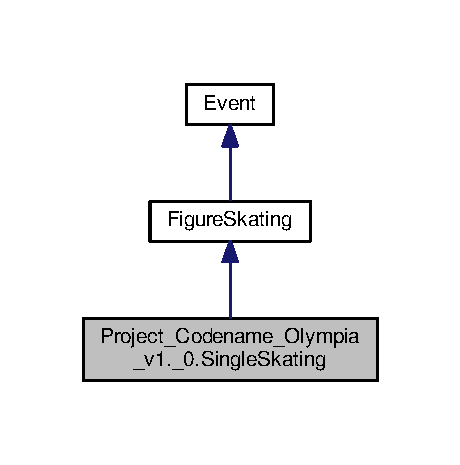
\includegraphics[width=221pt]{classProject__Codename__Olympia__v1_1_1__0_1_1SingleSkating__inherit__graph}
\end{center}
\end{figure}


Collaboration diagram for Project\+\_\+\+Codename\+\_\+\+Olympia\+\_\+v1.\+\_\+0.\+Single\+Skating\+:
\nopagebreak
\begin{figure}[H]
\begin{center}
\leavevmode
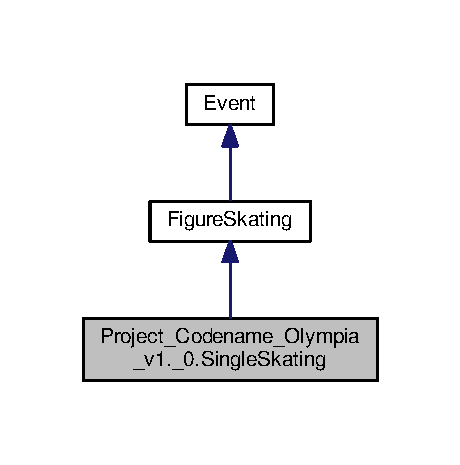
\includegraphics[width=221pt]{classProject__Codename__Olympia__v1_1_1__0_1_1SingleSkating__coll__graph}
\end{center}
\end{figure}
\subsection*{Public Member Functions}
\begin{DoxyCompactItemize}
\item 
\hyperlink{classProject__Codename__Olympia__v1_1_1__0_1_1SingleSkating_a89d99bd660975fdbe65fc0a1390caaea}{Single\+Skating} ()
\item 
override double \hyperlink{classProject__Codename__Olympia__v1_1_1__0_1_1SingleSkating_a0f1837cfe29187ca1c2402f6312f2465}{fs\+Score} ()
\item 
override int \hyperlink{classProject__Codename__Olympia__v1_1_1__0_1_1SingleSkating_a651ceefab408b4cbe3106ed7d673ba79}{event\+Num} ()
\item 
override void \hyperlink{classProject__Codename__Olympia__v1_1_1__0_1_1SingleSkating_abf63b846664f64fe96a68a05787f79aa}{run\+Event} (List$<$ \hyperlink{classProject__Codename__Olympia__v1_1_1__0_1_1Judge}{Judge} $>$ j, List$<$ \hyperlink{classProject__Codename__Olympia__v1_1_1__0_1_1Team}{Team} $>$ t)
\item 
override void \hyperlink{classProject__Codename__Olympia__v1_1_1__0_1_1SingleSkating_a481a432870964cfce7c319572c794a55}{sched\+Event} (List$<$ \hyperlink{classProject__Codename__Olympia__v1_1_1__0_1_1Judge}{Judge} $>$ j, List$<$ \hyperlink{classProject__Codename__Olympia__v1_1_1__0_1_1Team}{Team} $>$ t)
\end{DoxyCompactItemize}


\subsection{Detailed Description}
\hyperlink{classProject__Codename__Olympia__v1_1_1__0_1_1SingleSkating}{Single\+Skating} class is one of the 3 \hyperlink{classProject__Codename__Olympia__v1_1_1__0_1_1FigureSkating}{Figure\+Skating} events. 

D\+E\+F\+I\+N\+I\+T\+I\+ON\+: Form of figure skating where athletes participate individually. The utilization of long program style where each athlete is free to do their own unique performance complete with technical tricks is present.

C\+O\+N\+S\+T\+R\+A\+I\+N\+TS\+: Each athlete performs solo on the rink at a given time. Total duration of performance is 4 minutes and 30 seconds.\begin{DoxyAuthor}{Author}
Landen Marchand 
\end{DoxyAuthor}


\subsection{Constructor \& Destructor Documentation}
\mbox{\Hypertarget{classProject__Codename__Olympia__v1_1_1__0_1_1SingleSkating_a89d99bd660975fdbe65fc0a1390caaea}\label{classProject__Codename__Olympia__v1_1_1__0_1_1SingleSkating_a89d99bd660975fdbe65fc0a1390caaea}} 
\index{Project\+\_\+\+Codename\+\_\+\+Olympia\+\_\+v1\+::\+\_\+0\+::\+Single\+Skating@{Project\+\_\+\+Codename\+\_\+\+Olympia\+\_\+v1\+::\+\_\+0\+::\+Single\+Skating}!Single\+Skating@{Single\+Skating}}
\index{Single\+Skating@{Single\+Skating}!Project\+\_\+\+Codename\+\_\+\+Olympia\+\_\+v1\+::\+\_\+0\+::\+Single\+Skating@{Project\+\_\+\+Codename\+\_\+\+Olympia\+\_\+v1\+::\+\_\+0\+::\+Single\+Skating}}
\subsubsection{\texorpdfstring{Single\+Skating()}{SingleSkating()}}
{\footnotesize\ttfamily Project\+\_\+\+Codename\+\_\+\+Olympia\+\_\+v1.\+\_\+0.\+Single\+Skating.\+Single\+Skating (\begin{DoxyParamCaption}{ }\end{DoxyParamCaption})\hspace{0.3cm}{\ttfamily [inline]}}

Default Constructor Provided Automatically 
\begin{DoxyParams}{Parameters}
{\em None} & \\
\hline
\end{DoxyParams}
\begin{DoxyReturn}{Returns}
Default Values 
\end{DoxyReturn}


\subsection{Member Function Documentation}
\mbox{\Hypertarget{classProject__Codename__Olympia__v1_1_1__0_1_1SingleSkating_a651ceefab408b4cbe3106ed7d673ba79}\label{classProject__Codename__Olympia__v1_1_1__0_1_1SingleSkating_a651ceefab408b4cbe3106ed7d673ba79}} 
\index{Project\+\_\+\+Codename\+\_\+\+Olympia\+\_\+v1\+::\+\_\+0\+::\+Single\+Skating@{Project\+\_\+\+Codename\+\_\+\+Olympia\+\_\+v1\+::\+\_\+0\+::\+Single\+Skating}!event\+Num@{event\+Num}}
\index{event\+Num@{event\+Num}!Project\+\_\+\+Codename\+\_\+\+Olympia\+\_\+v1\+::\+\_\+0\+::\+Single\+Skating@{Project\+\_\+\+Codename\+\_\+\+Olympia\+\_\+v1\+::\+\_\+0\+::\+Single\+Skating}}
\subsubsection{\texorpdfstring{event\+Num()}{eventNum()}}
{\footnotesize\ttfamily override int Project\+\_\+\+Codename\+\_\+\+Olympia\+\_\+v1.\+\_\+0.\+Single\+Skating.\+event\+Num (\begin{DoxyParamCaption}{ }\end{DoxyParamCaption})\hspace{0.3cm}{\ttfamily [inline]}, {\ttfamily [virtual]}}

Function to override inherited \hyperlink{classProject__Codename__Olympia__v1_1_1__0_1_1SingleSkating_a651ceefab408b4cbe3106ed7d673ba79}{event\+Num()} function 

Implements \hyperlink{classProject__Codename__Olympia__v1_1_1__0_1_1Event_ad1154ef4dd1dec29d8ebf5614d84b1f3}{Project\+\_\+\+Codename\+\_\+\+Olympia\+\_\+v1.\+\_\+0.\+Event}.

\mbox{\Hypertarget{classProject__Codename__Olympia__v1_1_1__0_1_1SingleSkating_a0f1837cfe29187ca1c2402f6312f2465}\label{classProject__Codename__Olympia__v1_1_1__0_1_1SingleSkating_a0f1837cfe29187ca1c2402f6312f2465}} 
\index{Project\+\_\+\+Codename\+\_\+\+Olympia\+\_\+v1\+::\+\_\+0\+::\+Single\+Skating@{Project\+\_\+\+Codename\+\_\+\+Olympia\+\_\+v1\+::\+\_\+0\+::\+Single\+Skating}!fs\+Score@{fs\+Score}}
\index{fs\+Score@{fs\+Score}!Project\+\_\+\+Codename\+\_\+\+Olympia\+\_\+v1\+::\+\_\+0\+::\+Single\+Skating@{Project\+\_\+\+Codename\+\_\+\+Olympia\+\_\+v1\+::\+\_\+0\+::\+Single\+Skating}}
\subsubsection{\texorpdfstring{fs\+Score()}{fsScore()}}
{\footnotesize\ttfamily override double Project\+\_\+\+Codename\+\_\+\+Olympia\+\_\+v1.\+\_\+0.\+Single\+Skating.\+fs\+Score (\begin{DoxyParamCaption}{ }\end{DoxyParamCaption})\hspace{0.3cm}{\ttfamily [inline]}, {\ttfamily [virtual]}}

Function to override inherited \hyperlink{classProject__Codename__Olympia__v1_1_1__0_1_1SingleSkating_a0f1837cfe29187ca1c2402f6312f2465}{fs\+Score()} function 

Implements \hyperlink{classProject__Codename__Olympia__v1_1_1__0_1_1FigureSkating_a437e794fec382863421f8c65e31295f8}{Project\+\_\+\+Codename\+\_\+\+Olympia\+\_\+v1.\+\_\+0.\+Figure\+Skating}.

\mbox{\Hypertarget{classProject__Codename__Olympia__v1_1_1__0_1_1SingleSkating_abf63b846664f64fe96a68a05787f79aa}\label{classProject__Codename__Olympia__v1_1_1__0_1_1SingleSkating_abf63b846664f64fe96a68a05787f79aa}} 
\index{Project\+\_\+\+Codename\+\_\+\+Olympia\+\_\+v1\+::\+\_\+0\+::\+Single\+Skating@{Project\+\_\+\+Codename\+\_\+\+Olympia\+\_\+v1\+::\+\_\+0\+::\+Single\+Skating}!run\+Event@{run\+Event}}
\index{run\+Event@{run\+Event}!Project\+\_\+\+Codename\+\_\+\+Olympia\+\_\+v1\+::\+\_\+0\+::\+Single\+Skating@{Project\+\_\+\+Codename\+\_\+\+Olympia\+\_\+v1\+::\+\_\+0\+::\+Single\+Skating}}
\subsubsection{\texorpdfstring{run\+Event()}{runEvent()}}
{\footnotesize\ttfamily override void Project\+\_\+\+Codename\+\_\+\+Olympia\+\_\+v1.\+\_\+0.\+Single\+Skating.\+run\+Event (\begin{DoxyParamCaption}\item[{List$<$ \hyperlink{classProject__Codename__Olympia__v1_1_1__0_1_1Judge}{Judge} $>$}]{j,  }\item[{List$<$ \hyperlink{classProject__Codename__Olympia__v1_1_1__0_1_1Team}{Team} $>$}]{t }\end{DoxyParamCaption})\hspace{0.3cm}{\ttfamily [inline]}, {\ttfamily [virtual]}}

Function to override inherited run\+Event(..) function 

Implements \hyperlink{classProject__Codename__Olympia__v1_1_1__0_1_1Event_ac6ff060da23153c02da49937dcf9f326}{Project\+\_\+\+Codename\+\_\+\+Olympia\+\_\+v1.\+\_\+0.\+Event}.

\mbox{\Hypertarget{classProject__Codename__Olympia__v1_1_1__0_1_1SingleSkating_a481a432870964cfce7c319572c794a55}\label{classProject__Codename__Olympia__v1_1_1__0_1_1SingleSkating_a481a432870964cfce7c319572c794a55}} 
\index{Project\+\_\+\+Codename\+\_\+\+Olympia\+\_\+v1\+::\+\_\+0\+::\+Single\+Skating@{Project\+\_\+\+Codename\+\_\+\+Olympia\+\_\+v1\+::\+\_\+0\+::\+Single\+Skating}!sched\+Event@{sched\+Event}}
\index{sched\+Event@{sched\+Event}!Project\+\_\+\+Codename\+\_\+\+Olympia\+\_\+v1\+::\+\_\+0\+::\+Single\+Skating@{Project\+\_\+\+Codename\+\_\+\+Olympia\+\_\+v1\+::\+\_\+0\+::\+Single\+Skating}}
\subsubsection{\texorpdfstring{sched\+Event()}{schedEvent()}}
{\footnotesize\ttfamily override void Project\+\_\+\+Codename\+\_\+\+Olympia\+\_\+v1.\+\_\+0.\+Single\+Skating.\+sched\+Event (\begin{DoxyParamCaption}\item[{List$<$ \hyperlink{classProject__Codename__Olympia__v1_1_1__0_1_1Judge}{Judge} $>$}]{j,  }\item[{List$<$ \hyperlink{classProject__Codename__Olympia__v1_1_1__0_1_1Team}{Team} $>$}]{t }\end{DoxyParamCaption})\hspace{0.3cm}{\ttfamily [inline]}, {\ttfamily [virtual]}}

Function to override inherited sched\+Event(..) function 

Implements \hyperlink{classProject__Codename__Olympia__v1_1_1__0_1_1Event_abb4e2b9c28527b9a28395f2fe9192196}{Project\+\_\+\+Codename\+\_\+\+Olympia\+\_\+v1.\+\_\+0.\+Event}.



The documentation for this class was generated from the following file\+:\begin{DoxyCompactItemize}
\item 
Class1.\+cs\end{DoxyCompactItemize}

\hypertarget{classProject__Codename__Olympia__v1_1_1__0_1_1SpeedSkating}{}\section{Project\+\_\+\+Codename\+\_\+\+Olympia\+\_\+v1.\+\_\+0.\+Speed\+Skating Class Reference}
\label{classProject__Codename__Olympia__v1_1_1__0_1_1SpeedSkating}\index{Project\+\_\+\+Codename\+\_\+\+Olympia\+\_\+v1.\+\_\+0.\+Speed\+Skating@{Project\+\_\+\+Codename\+\_\+\+Olympia\+\_\+v1.\+\_\+0.\+Speed\+Skating}}


\hyperlink{classProject__Codename__Olympia__v1_1_1__0_1_1SpeedSkating}{Speed\+Skating} class is the superclass of the 3 \hyperlink{classProject__Codename__Olympia__v1_1_1__0_1_1SpeedSkating}{Speed\+Skating} events.  




Inheritance diagram for Project\+\_\+\+Codename\+\_\+\+Olympia\+\_\+v1.\+\_\+0.\+Speed\+Skating\+:
\nopagebreak
\begin{figure}[H]
\begin{center}
\leavevmode
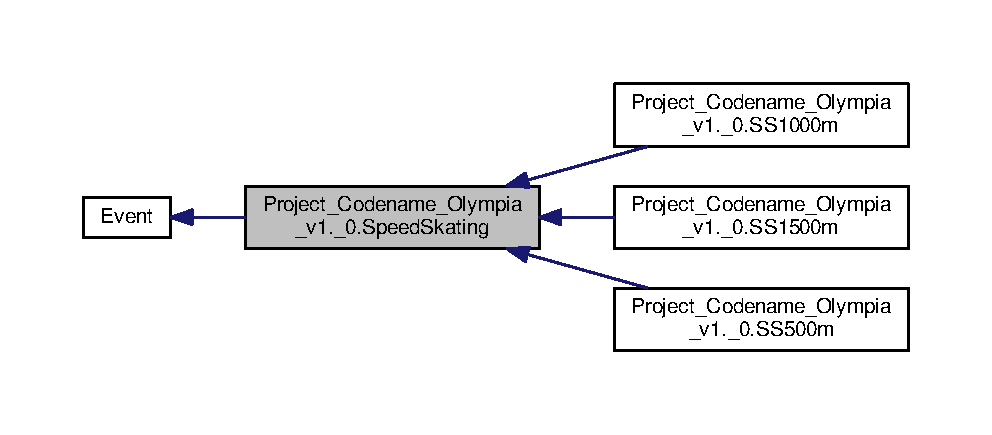
\includegraphics[width=350pt]{classProject__Codename__Olympia__v1_1_1__0_1_1SpeedSkating__inherit__graph}
\end{center}
\end{figure}


Collaboration diagram for Project\+\_\+\+Codename\+\_\+\+Olympia\+\_\+v1.\+\_\+0.\+Speed\+Skating\+:
\nopagebreak
\begin{figure}[H]
\begin{center}
\leavevmode
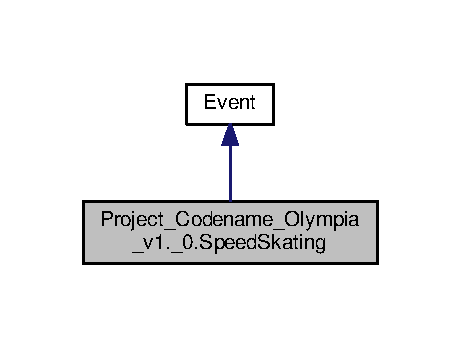
\includegraphics[width=221pt]{classProject__Codename__Olympia__v1_1_1__0_1_1SpeedSkating__coll__graph}
\end{center}
\end{figure}
\subsection*{Classes}
\begin{DoxyCompactItemize}
\item 
interface \hyperlink{interfaceProject__Codename__Olympia__v1_1_1__0_1_1SpeedSkating_1_1ssInheritance}{ss\+Inheritance}
\end{DoxyCompactItemize}
\subsection*{Public Member Functions}
\begin{DoxyCompactItemize}
\item 
\hyperlink{classProject__Codename__Olympia__v1_1_1__0_1_1SpeedSkating_af596581bdbb1d5e6a5d95cd1f887169b}{Speed\+Skating} ()
\item 
abstract double \hyperlink{classProject__Codename__Olympia__v1_1_1__0_1_1SpeedSkating_acedc7b2f1bfab95ee054531364ea50fb}{ss\+Time} ()
\end{DoxyCompactItemize}


\subsection{Detailed Description}
\hyperlink{classProject__Codename__Olympia__v1_1_1__0_1_1SpeedSkating}{Speed\+Skating} class is the superclass of the 3 \hyperlink{classProject__Codename__Olympia__v1_1_1__0_1_1SpeedSkating}{Speed\+Skating} events. 

D\+E\+F\+I\+N\+T\+I\+ON\+: Skating done on ice at a fast pace around an oval track utilizing inline skates where scoring is based upon time. One of the two main sporting categories that consist of three unique events which athletes participate separately.

C\+O\+N\+S\+T\+R\+A\+I\+N\+TS\+: None\begin{DoxyAuthor}{Author}
Landen Marchand 
\end{DoxyAuthor}


\subsection{Constructor \& Destructor Documentation}
\mbox{\Hypertarget{classProject__Codename__Olympia__v1_1_1__0_1_1SpeedSkating_af596581bdbb1d5e6a5d95cd1f887169b}\label{classProject__Codename__Olympia__v1_1_1__0_1_1SpeedSkating_af596581bdbb1d5e6a5d95cd1f887169b}} 
\index{Project\+\_\+\+Codename\+\_\+\+Olympia\+\_\+v1\+::\+\_\+0\+::\+Speed\+Skating@{Project\+\_\+\+Codename\+\_\+\+Olympia\+\_\+v1\+::\+\_\+0\+::\+Speed\+Skating}!Speed\+Skating@{Speed\+Skating}}
\index{Speed\+Skating@{Speed\+Skating}!Project\+\_\+\+Codename\+\_\+\+Olympia\+\_\+v1\+::\+\_\+0\+::\+Speed\+Skating@{Project\+\_\+\+Codename\+\_\+\+Olympia\+\_\+v1\+::\+\_\+0\+::\+Speed\+Skating}}
\subsubsection{\texorpdfstring{Speed\+Skating()}{SpeedSkating()}}
{\footnotesize\ttfamily Project\+\_\+\+Codename\+\_\+\+Olympia\+\_\+v1.\+\_\+0.\+Speed\+Skating.\+Speed\+Skating (\begin{DoxyParamCaption}{ }\end{DoxyParamCaption})\hspace{0.3cm}{\ttfamily [inline]}}

Default Constructor Provided Automatically 
\begin{DoxyParams}{Parameters}
{\em None} & \\
\hline
\end{DoxyParams}
\begin{DoxyReturn}{Returns}
Default Values 
\end{DoxyReturn}


\subsection{Member Function Documentation}
\mbox{\Hypertarget{classProject__Codename__Olympia__v1_1_1__0_1_1SpeedSkating_acedc7b2f1bfab95ee054531364ea50fb}\label{classProject__Codename__Olympia__v1_1_1__0_1_1SpeedSkating_acedc7b2f1bfab95ee054531364ea50fb}} 
\index{Project\+\_\+\+Codename\+\_\+\+Olympia\+\_\+v1\+::\+\_\+0\+::\+Speed\+Skating@{Project\+\_\+\+Codename\+\_\+\+Olympia\+\_\+v1\+::\+\_\+0\+::\+Speed\+Skating}!ss\+Time@{ss\+Time}}
\index{ss\+Time@{ss\+Time}!Project\+\_\+\+Codename\+\_\+\+Olympia\+\_\+v1\+::\+\_\+0\+::\+Speed\+Skating@{Project\+\_\+\+Codename\+\_\+\+Olympia\+\_\+v1\+::\+\_\+0\+::\+Speed\+Skating}}
\subsubsection{\texorpdfstring{ss\+Time()}{ssTime()}}
{\footnotesize\ttfamily abstract double Project\+\_\+\+Codename\+\_\+\+Olympia\+\_\+v1.\+\_\+0.\+Speed\+Skating.\+ss\+Time (\begin{DoxyParamCaption}{ }\end{DoxyParamCaption})\hspace{0.3cm}{\ttfamily [pure virtual]}}

Inheritance member function for \hyperlink{classProject__Codename__Olympia__v1_1_1__0_1_1SpeedSkating}{Speed\+Skating} events 
\begin{DoxyParams}{Parameters}
{\em none} & \\
\hline
\end{DoxyParams}
\begin{DoxyReturn}{Returns}
double pertaining to time (completion of event of athlete) 
\end{DoxyReturn}


Implemented in \hyperlink{classProject__Codename__Olympia__v1_1_1__0_1_1SS500m_a1fc1ed5e2b6d1fa4d1921a3d155c6a6f}{Project\+\_\+\+Codename\+\_\+\+Olympia\+\_\+v1.\+\_\+0.\+S\+S500m}, \hyperlink{classProject__Codename__Olympia__v1_1_1__0_1_1SS1500m_a70484e4f6b73c271756fa9bb6950eb0b}{Project\+\_\+\+Codename\+\_\+\+Olympia\+\_\+v1.\+\_\+0.\+S\+S1500m}, and \hyperlink{classProject__Codename__Olympia__v1_1_1__0_1_1SS1000m_a4bfd83bce70e047370288c0b651e3e1c}{Project\+\_\+\+Codename\+\_\+\+Olympia\+\_\+v1.\+\_\+0.\+S\+S1000m}.



The documentation for this class was generated from the following file\+:\begin{DoxyCompactItemize}
\item 
Class1.\+cs\end{DoxyCompactItemize}

\hypertarget{classProject__Codename__Olympia__v1_1_1__0_1_1SS1000m}{}\section{Project\+\_\+\+Codename\+\_\+\+Olympia\+\_\+v1.\+\_\+0.\+S\+S1000m Class Reference}
\label{classProject__Codename__Olympia__v1_1_1__0_1_1SS1000m}\index{Project\+\_\+\+Codename\+\_\+\+Olympia\+\_\+v1.\+\_\+0.\+S\+S1000m@{Project\+\_\+\+Codename\+\_\+\+Olympia\+\_\+v1.\+\_\+0.\+S\+S1000m}}


\hyperlink{classProject__Codename__Olympia__v1_1_1__0_1_1SS1000m}{S\+S1000m} is one of the 3 \hyperlink{classProject__Codename__Olympia__v1_1_1__0_1_1SpeedSkating}{Speed\+Skating} events.  




Inheritance diagram for Project\+\_\+\+Codename\+\_\+\+Olympia\+\_\+v1.\+\_\+0.\+S\+S1000m\+:
\nopagebreak
\begin{figure}[H]
\begin{center}
\leavevmode
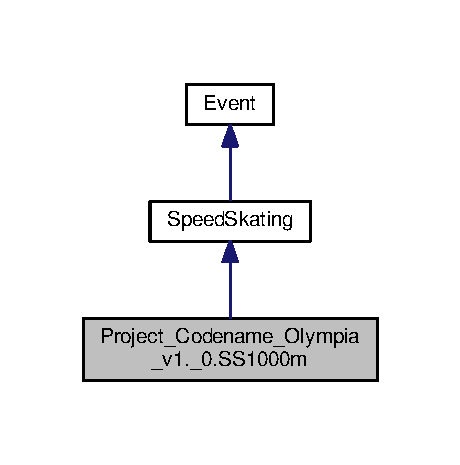
\includegraphics[width=221pt]{classProject__Codename__Olympia__v1_1_1__0_1_1SS1000m__inherit__graph}
\end{center}
\end{figure}


Collaboration diagram for Project\+\_\+\+Codename\+\_\+\+Olympia\+\_\+v1.\+\_\+0.\+S\+S1000m\+:
\nopagebreak
\begin{figure}[H]
\begin{center}
\leavevmode
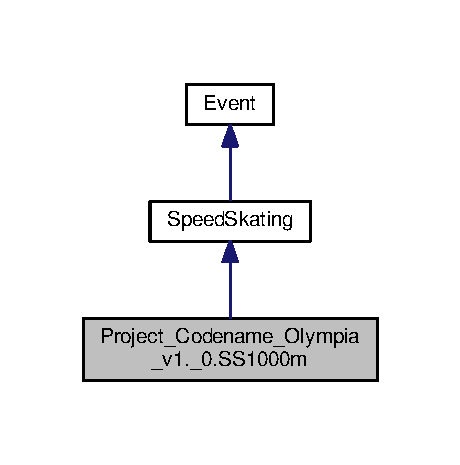
\includegraphics[width=221pt]{classProject__Codename__Olympia__v1_1_1__0_1_1SS1000m__coll__graph}
\end{center}
\end{figure}
\subsection*{Public Member Functions}
\begin{DoxyCompactItemize}
\item 
\hyperlink{classProject__Codename__Olympia__v1_1_1__0_1_1SS1000m_af0de8059e97b8a3fc6f304d532b6f89b}{S\+S1000m} ()
\item 
override double \hyperlink{classProject__Codename__Olympia__v1_1_1__0_1_1SS1000m_a4bfd83bce70e047370288c0b651e3e1c}{ss\+Time} ()
\item 
override int \hyperlink{classProject__Codename__Olympia__v1_1_1__0_1_1SS1000m_aea0a2bb558a0b5f1ee0cae54a9e12ea9}{event\+Num} ()
\item 
override void \hyperlink{classProject__Codename__Olympia__v1_1_1__0_1_1SS1000m_ab08df1d91a7685c6d1dc9bdec0d45fba}{run\+Event} (List$<$ \hyperlink{classProject__Codename__Olympia__v1_1_1__0_1_1Judge}{Judge} $>$ j, List$<$ \hyperlink{classProject__Codename__Olympia__v1_1_1__0_1_1Team}{Team} $>$ t)
\item 
override void \hyperlink{classProject__Codename__Olympia__v1_1_1__0_1_1SS1000m_a4cb7d76aed8d478577e243b187ce4830}{sched\+Event} (List$<$ \hyperlink{classProject__Codename__Olympia__v1_1_1__0_1_1Judge}{Judge} $>$ j, List$<$ \hyperlink{classProject__Codename__Olympia__v1_1_1__0_1_1Team}{Team} $>$ t)
\end{DoxyCompactItemize}


\subsection{Detailed Description}
\hyperlink{classProject__Codename__Olympia__v1_1_1__0_1_1SS1000m}{S\+S1000m} is one of the 3 \hyperlink{classProject__Codename__Olympia__v1_1_1__0_1_1SpeedSkating}{Speed\+Skating} events. 

D\+E\+F\+I\+N\+T\+I\+ON\+: Form of speed skating where athletes utilize inline skates and race around a 400m rink 2.\+5 times. Whichever athlete crosses the finish line first has the lowest time.

C\+O\+N\+S\+T\+R\+A\+I\+N\+TS\+: A maximum of four athletes compete at a given time.\begin{DoxyAuthor}{Author}
Landen Marchand 
\end{DoxyAuthor}


\subsection{Constructor \& Destructor Documentation}
\mbox{\Hypertarget{classProject__Codename__Olympia__v1_1_1__0_1_1SS1000m_af0de8059e97b8a3fc6f304d532b6f89b}\label{classProject__Codename__Olympia__v1_1_1__0_1_1SS1000m_af0de8059e97b8a3fc6f304d532b6f89b}} 
\index{Project\+\_\+\+Codename\+\_\+\+Olympia\+\_\+v1\+::\+\_\+0\+::\+S\+S1000m@{Project\+\_\+\+Codename\+\_\+\+Olympia\+\_\+v1\+::\+\_\+0\+::\+S\+S1000m}!S\+S1000m@{S\+S1000m}}
\index{S\+S1000m@{S\+S1000m}!Project\+\_\+\+Codename\+\_\+\+Olympia\+\_\+v1\+::\+\_\+0\+::\+S\+S1000m@{Project\+\_\+\+Codename\+\_\+\+Olympia\+\_\+v1\+::\+\_\+0\+::\+S\+S1000m}}
\subsubsection{\texorpdfstring{S\+S1000m()}{SS1000m()}}
{\footnotesize\ttfamily Project\+\_\+\+Codename\+\_\+\+Olympia\+\_\+v1.\+\_\+0.\+S\+S1000m.\+S\+S1000m (\begin{DoxyParamCaption}{ }\end{DoxyParamCaption})\hspace{0.3cm}{\ttfamily [inline]}}

Default Constructor Provided Automatically 
\begin{DoxyParams}{Parameters}
{\em None} & \\
\hline
\end{DoxyParams}
\begin{DoxyReturn}{Returns}
Default Values 
\end{DoxyReturn}


\subsection{Member Function Documentation}
\mbox{\Hypertarget{classProject__Codename__Olympia__v1_1_1__0_1_1SS1000m_aea0a2bb558a0b5f1ee0cae54a9e12ea9}\label{classProject__Codename__Olympia__v1_1_1__0_1_1SS1000m_aea0a2bb558a0b5f1ee0cae54a9e12ea9}} 
\index{Project\+\_\+\+Codename\+\_\+\+Olympia\+\_\+v1\+::\+\_\+0\+::\+S\+S1000m@{Project\+\_\+\+Codename\+\_\+\+Olympia\+\_\+v1\+::\+\_\+0\+::\+S\+S1000m}!event\+Num@{event\+Num}}
\index{event\+Num@{event\+Num}!Project\+\_\+\+Codename\+\_\+\+Olympia\+\_\+v1\+::\+\_\+0\+::\+S\+S1000m@{Project\+\_\+\+Codename\+\_\+\+Olympia\+\_\+v1\+::\+\_\+0\+::\+S\+S1000m}}
\subsubsection{\texorpdfstring{event\+Num()}{eventNum()}}
{\footnotesize\ttfamily override int Project\+\_\+\+Codename\+\_\+\+Olympia\+\_\+v1.\+\_\+0.\+S\+S1000m.\+event\+Num (\begin{DoxyParamCaption}{ }\end{DoxyParamCaption})\hspace{0.3cm}{\ttfamily [inline]}, {\ttfamily [virtual]}}

Function to override inherited \hyperlink{classProject__Codename__Olympia__v1_1_1__0_1_1SS1000m_aea0a2bb558a0b5f1ee0cae54a9e12ea9}{event\+Num()} function 

Implements \hyperlink{classProject__Codename__Olympia__v1_1_1__0_1_1Event_ad1154ef4dd1dec29d8ebf5614d84b1f3}{Project\+\_\+\+Codename\+\_\+\+Olympia\+\_\+v1.\+\_\+0.\+Event}.

\mbox{\Hypertarget{classProject__Codename__Olympia__v1_1_1__0_1_1SS1000m_ab08df1d91a7685c6d1dc9bdec0d45fba}\label{classProject__Codename__Olympia__v1_1_1__0_1_1SS1000m_ab08df1d91a7685c6d1dc9bdec0d45fba}} 
\index{Project\+\_\+\+Codename\+\_\+\+Olympia\+\_\+v1\+::\+\_\+0\+::\+S\+S1000m@{Project\+\_\+\+Codename\+\_\+\+Olympia\+\_\+v1\+::\+\_\+0\+::\+S\+S1000m}!run\+Event@{run\+Event}}
\index{run\+Event@{run\+Event}!Project\+\_\+\+Codename\+\_\+\+Olympia\+\_\+v1\+::\+\_\+0\+::\+S\+S1000m@{Project\+\_\+\+Codename\+\_\+\+Olympia\+\_\+v1\+::\+\_\+0\+::\+S\+S1000m}}
\subsubsection{\texorpdfstring{run\+Event()}{runEvent()}}
{\footnotesize\ttfamily override void Project\+\_\+\+Codename\+\_\+\+Olympia\+\_\+v1.\+\_\+0.\+S\+S1000m.\+run\+Event (\begin{DoxyParamCaption}\item[{List$<$ \hyperlink{classProject__Codename__Olympia__v1_1_1__0_1_1Judge}{Judge} $>$}]{j,  }\item[{List$<$ \hyperlink{classProject__Codename__Olympia__v1_1_1__0_1_1Team}{Team} $>$}]{t }\end{DoxyParamCaption})\hspace{0.3cm}{\ttfamily [inline]}, {\ttfamily [virtual]}}

Function to override inherited run\+Event(..) function 

Implements \hyperlink{classProject__Codename__Olympia__v1_1_1__0_1_1Event_ac6ff060da23153c02da49937dcf9f326}{Project\+\_\+\+Codename\+\_\+\+Olympia\+\_\+v1.\+\_\+0.\+Event}.

\mbox{\Hypertarget{classProject__Codename__Olympia__v1_1_1__0_1_1SS1000m_a4cb7d76aed8d478577e243b187ce4830}\label{classProject__Codename__Olympia__v1_1_1__0_1_1SS1000m_a4cb7d76aed8d478577e243b187ce4830}} 
\index{Project\+\_\+\+Codename\+\_\+\+Olympia\+\_\+v1\+::\+\_\+0\+::\+S\+S1000m@{Project\+\_\+\+Codename\+\_\+\+Olympia\+\_\+v1\+::\+\_\+0\+::\+S\+S1000m}!sched\+Event@{sched\+Event}}
\index{sched\+Event@{sched\+Event}!Project\+\_\+\+Codename\+\_\+\+Olympia\+\_\+v1\+::\+\_\+0\+::\+S\+S1000m@{Project\+\_\+\+Codename\+\_\+\+Olympia\+\_\+v1\+::\+\_\+0\+::\+S\+S1000m}}
\subsubsection{\texorpdfstring{sched\+Event()}{schedEvent()}}
{\footnotesize\ttfamily override void Project\+\_\+\+Codename\+\_\+\+Olympia\+\_\+v1.\+\_\+0.\+S\+S1000m.\+sched\+Event (\begin{DoxyParamCaption}\item[{List$<$ \hyperlink{classProject__Codename__Olympia__v1_1_1__0_1_1Judge}{Judge} $>$}]{j,  }\item[{List$<$ \hyperlink{classProject__Codename__Olympia__v1_1_1__0_1_1Team}{Team} $>$}]{t }\end{DoxyParamCaption})\hspace{0.3cm}{\ttfamily [inline]}, {\ttfamily [virtual]}}

Function to override inherited sched\+Event(..) function 

Implements \hyperlink{classProject__Codename__Olympia__v1_1_1__0_1_1Event_abb4e2b9c28527b9a28395f2fe9192196}{Project\+\_\+\+Codename\+\_\+\+Olympia\+\_\+v1.\+\_\+0.\+Event}.

\mbox{\Hypertarget{classProject__Codename__Olympia__v1_1_1__0_1_1SS1000m_a4bfd83bce70e047370288c0b651e3e1c}\label{classProject__Codename__Olympia__v1_1_1__0_1_1SS1000m_a4bfd83bce70e047370288c0b651e3e1c}} 
\index{Project\+\_\+\+Codename\+\_\+\+Olympia\+\_\+v1\+::\+\_\+0\+::\+S\+S1000m@{Project\+\_\+\+Codename\+\_\+\+Olympia\+\_\+v1\+::\+\_\+0\+::\+S\+S1000m}!ss\+Time@{ss\+Time}}
\index{ss\+Time@{ss\+Time}!Project\+\_\+\+Codename\+\_\+\+Olympia\+\_\+v1\+::\+\_\+0\+::\+S\+S1000m@{Project\+\_\+\+Codename\+\_\+\+Olympia\+\_\+v1\+::\+\_\+0\+::\+S\+S1000m}}
\subsubsection{\texorpdfstring{ss\+Time()}{ssTime()}}
{\footnotesize\ttfamily override double Project\+\_\+\+Codename\+\_\+\+Olympia\+\_\+v1.\+\_\+0.\+S\+S1000m.\+ss\+Time (\begin{DoxyParamCaption}{ }\end{DoxyParamCaption})\hspace{0.3cm}{\ttfamily [inline]}, {\ttfamily [virtual]}}

Function to override inherited \hyperlink{classProject__Codename__Olympia__v1_1_1__0_1_1SS1000m_a4bfd83bce70e047370288c0b651e3e1c}{ss\+Time()} function 

Implements \hyperlink{classProject__Codename__Olympia__v1_1_1__0_1_1SpeedSkating_acedc7b2f1bfab95ee054531364ea50fb}{Project\+\_\+\+Codename\+\_\+\+Olympia\+\_\+v1.\+\_\+0.\+Speed\+Skating}.



The documentation for this class was generated from the following file\+:\begin{DoxyCompactItemize}
\item 
Class1.\+cs\end{DoxyCompactItemize}

\hypertarget{classProject__Codename__Olympia__v1_1_1__0_1_1SS1500m}{}\section{Project\+\_\+\+Codename\+\_\+\+Olympia\+\_\+v1.\+\_\+0.\+S\+S1500m Class Reference}
\label{classProject__Codename__Olympia__v1_1_1__0_1_1SS1500m}\index{Project\+\_\+\+Codename\+\_\+\+Olympia\+\_\+v1.\+\_\+0.\+S\+S1500m@{Project\+\_\+\+Codename\+\_\+\+Olympia\+\_\+v1.\+\_\+0.\+S\+S1500m}}


\hyperlink{classProject__Codename__Olympia__v1_1_1__0_1_1SS1500m}{S\+S1500m} is one of the 3 \hyperlink{classProject__Codename__Olympia__v1_1_1__0_1_1SpeedSkating}{Speed\+Skating} events.  




Inheritance diagram for Project\+\_\+\+Codename\+\_\+\+Olympia\+\_\+v1.\+\_\+0.\+S\+S1500m\+:
\nopagebreak
\begin{figure}[H]
\begin{center}
\leavevmode
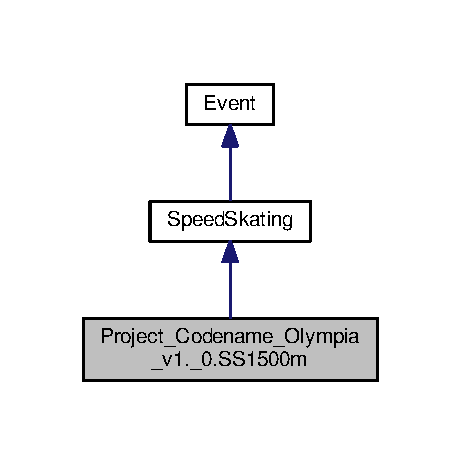
\includegraphics[width=221pt]{classProject__Codename__Olympia__v1_1_1__0_1_1SS1500m__inherit__graph}
\end{center}
\end{figure}


Collaboration diagram for Project\+\_\+\+Codename\+\_\+\+Olympia\+\_\+v1.\+\_\+0.\+S\+S1500m\+:
\nopagebreak
\begin{figure}[H]
\begin{center}
\leavevmode
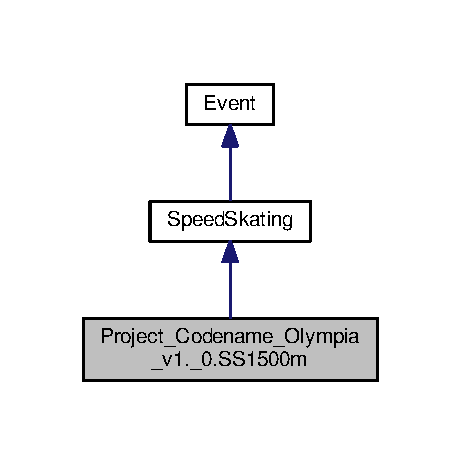
\includegraphics[width=221pt]{classProject__Codename__Olympia__v1_1_1__0_1_1SS1500m__coll__graph}
\end{center}
\end{figure}
\subsection*{Public Member Functions}
\begin{DoxyCompactItemize}
\item 
\hyperlink{classProject__Codename__Olympia__v1_1_1__0_1_1SS1500m_a86936a68b36ff296c67b067a73ed90bd}{S\+S1500m} ()
\item 
override double \hyperlink{classProject__Codename__Olympia__v1_1_1__0_1_1SS1500m_a70484e4f6b73c271756fa9bb6950eb0b}{ss\+Time} ()
\item 
override int \hyperlink{classProject__Codename__Olympia__v1_1_1__0_1_1SS1500m_a012967ff7e84eb9d1578705ad465aecc}{event\+Num} ()
\item 
override void \hyperlink{classProject__Codename__Olympia__v1_1_1__0_1_1SS1500m_a749ab5adb7bd98da6e7370fef95d46fd}{run\+Event} (List$<$ \hyperlink{classProject__Codename__Olympia__v1_1_1__0_1_1Judge}{Judge} $>$ j, List$<$ \hyperlink{classProject__Codename__Olympia__v1_1_1__0_1_1Team}{Team} $>$ t)
\item 
override void \hyperlink{classProject__Codename__Olympia__v1_1_1__0_1_1SS1500m_af87bf024ce84968289b999323d1a53bb}{sched\+Event} (List$<$ \hyperlink{classProject__Codename__Olympia__v1_1_1__0_1_1Judge}{Judge} $>$ j, List$<$ \hyperlink{classProject__Codename__Olympia__v1_1_1__0_1_1Team}{Team} $>$ t)
\end{DoxyCompactItemize}


\subsection{Detailed Description}
\hyperlink{classProject__Codename__Olympia__v1_1_1__0_1_1SS1500m}{S\+S1500m} is one of the 3 \hyperlink{classProject__Codename__Olympia__v1_1_1__0_1_1SpeedSkating}{Speed\+Skating} events. 

D\+E\+F\+I\+N\+T\+I\+ON\+: Form of speed skating where athletes utilize inline skates and race around a 400m rink 3.\+75 times. Whichever athlete crosses the finish line first has the lowest time.

C\+O\+N\+S\+T\+R\+A\+I\+NS\+: A maximum of four athletes compete at a given time.\begin{DoxyAuthor}{Author}
Landen Marchand 
\end{DoxyAuthor}


\subsection{Constructor \& Destructor Documentation}
\mbox{\Hypertarget{classProject__Codename__Olympia__v1_1_1__0_1_1SS1500m_a86936a68b36ff296c67b067a73ed90bd}\label{classProject__Codename__Olympia__v1_1_1__0_1_1SS1500m_a86936a68b36ff296c67b067a73ed90bd}} 
\index{Project\+\_\+\+Codename\+\_\+\+Olympia\+\_\+v1\+::\+\_\+0\+::\+S\+S1500m@{Project\+\_\+\+Codename\+\_\+\+Olympia\+\_\+v1\+::\+\_\+0\+::\+S\+S1500m}!S\+S1500m@{S\+S1500m}}
\index{S\+S1500m@{S\+S1500m}!Project\+\_\+\+Codename\+\_\+\+Olympia\+\_\+v1\+::\+\_\+0\+::\+S\+S1500m@{Project\+\_\+\+Codename\+\_\+\+Olympia\+\_\+v1\+::\+\_\+0\+::\+S\+S1500m}}
\subsubsection{\texorpdfstring{S\+S1500m()}{SS1500m()}}
{\footnotesize\ttfamily Project\+\_\+\+Codename\+\_\+\+Olympia\+\_\+v1.\+\_\+0.\+S\+S1500m.\+S\+S1500m (\begin{DoxyParamCaption}{ }\end{DoxyParamCaption})\hspace{0.3cm}{\ttfamily [inline]}}

Default Constructor Provided Automatically 
\begin{DoxyParams}{Parameters}
{\em None} & \\
\hline
\end{DoxyParams}
\begin{DoxyReturn}{Returns}
Default Values 
\end{DoxyReturn}


\subsection{Member Function Documentation}
\mbox{\Hypertarget{classProject__Codename__Olympia__v1_1_1__0_1_1SS1500m_a012967ff7e84eb9d1578705ad465aecc}\label{classProject__Codename__Olympia__v1_1_1__0_1_1SS1500m_a012967ff7e84eb9d1578705ad465aecc}} 
\index{Project\+\_\+\+Codename\+\_\+\+Olympia\+\_\+v1\+::\+\_\+0\+::\+S\+S1500m@{Project\+\_\+\+Codename\+\_\+\+Olympia\+\_\+v1\+::\+\_\+0\+::\+S\+S1500m}!event\+Num@{event\+Num}}
\index{event\+Num@{event\+Num}!Project\+\_\+\+Codename\+\_\+\+Olympia\+\_\+v1\+::\+\_\+0\+::\+S\+S1500m@{Project\+\_\+\+Codename\+\_\+\+Olympia\+\_\+v1\+::\+\_\+0\+::\+S\+S1500m}}
\subsubsection{\texorpdfstring{event\+Num()}{eventNum()}}
{\footnotesize\ttfamily override int Project\+\_\+\+Codename\+\_\+\+Olympia\+\_\+v1.\+\_\+0.\+S\+S1500m.\+event\+Num (\begin{DoxyParamCaption}{ }\end{DoxyParamCaption})\hspace{0.3cm}{\ttfamily [inline]}, {\ttfamily [virtual]}}

Function to override inherited \hyperlink{classProject__Codename__Olympia__v1_1_1__0_1_1SS1500m_a012967ff7e84eb9d1578705ad465aecc}{event\+Num()} function 

Implements \hyperlink{classProject__Codename__Olympia__v1_1_1__0_1_1Event_ad1154ef4dd1dec29d8ebf5614d84b1f3}{Project\+\_\+\+Codename\+\_\+\+Olympia\+\_\+v1.\+\_\+0.\+Event}.

\mbox{\Hypertarget{classProject__Codename__Olympia__v1_1_1__0_1_1SS1500m_a749ab5adb7bd98da6e7370fef95d46fd}\label{classProject__Codename__Olympia__v1_1_1__0_1_1SS1500m_a749ab5adb7bd98da6e7370fef95d46fd}} 
\index{Project\+\_\+\+Codename\+\_\+\+Olympia\+\_\+v1\+::\+\_\+0\+::\+S\+S1500m@{Project\+\_\+\+Codename\+\_\+\+Olympia\+\_\+v1\+::\+\_\+0\+::\+S\+S1500m}!run\+Event@{run\+Event}}
\index{run\+Event@{run\+Event}!Project\+\_\+\+Codename\+\_\+\+Olympia\+\_\+v1\+::\+\_\+0\+::\+S\+S1500m@{Project\+\_\+\+Codename\+\_\+\+Olympia\+\_\+v1\+::\+\_\+0\+::\+S\+S1500m}}
\subsubsection{\texorpdfstring{run\+Event()}{runEvent()}}
{\footnotesize\ttfamily override void Project\+\_\+\+Codename\+\_\+\+Olympia\+\_\+v1.\+\_\+0.\+S\+S1500m.\+run\+Event (\begin{DoxyParamCaption}\item[{List$<$ \hyperlink{classProject__Codename__Olympia__v1_1_1__0_1_1Judge}{Judge} $>$}]{j,  }\item[{List$<$ \hyperlink{classProject__Codename__Olympia__v1_1_1__0_1_1Team}{Team} $>$}]{t }\end{DoxyParamCaption})\hspace{0.3cm}{\ttfamily [inline]}, {\ttfamily [virtual]}}

Function to override inherited run\+Event(..) function 

Implements \hyperlink{classProject__Codename__Olympia__v1_1_1__0_1_1Event_ac6ff060da23153c02da49937dcf9f326}{Project\+\_\+\+Codename\+\_\+\+Olympia\+\_\+v1.\+\_\+0.\+Event}.

\mbox{\Hypertarget{classProject__Codename__Olympia__v1_1_1__0_1_1SS1500m_af87bf024ce84968289b999323d1a53bb}\label{classProject__Codename__Olympia__v1_1_1__0_1_1SS1500m_af87bf024ce84968289b999323d1a53bb}} 
\index{Project\+\_\+\+Codename\+\_\+\+Olympia\+\_\+v1\+::\+\_\+0\+::\+S\+S1500m@{Project\+\_\+\+Codename\+\_\+\+Olympia\+\_\+v1\+::\+\_\+0\+::\+S\+S1500m}!sched\+Event@{sched\+Event}}
\index{sched\+Event@{sched\+Event}!Project\+\_\+\+Codename\+\_\+\+Olympia\+\_\+v1\+::\+\_\+0\+::\+S\+S1500m@{Project\+\_\+\+Codename\+\_\+\+Olympia\+\_\+v1\+::\+\_\+0\+::\+S\+S1500m}}
\subsubsection{\texorpdfstring{sched\+Event()}{schedEvent()}}
{\footnotesize\ttfamily override void Project\+\_\+\+Codename\+\_\+\+Olympia\+\_\+v1.\+\_\+0.\+S\+S1500m.\+sched\+Event (\begin{DoxyParamCaption}\item[{List$<$ \hyperlink{classProject__Codename__Olympia__v1_1_1__0_1_1Judge}{Judge} $>$}]{j,  }\item[{List$<$ \hyperlink{classProject__Codename__Olympia__v1_1_1__0_1_1Team}{Team} $>$}]{t }\end{DoxyParamCaption})\hspace{0.3cm}{\ttfamily [inline]}, {\ttfamily [virtual]}}

Function to override inherited sched\+Event(..) function 

Implements \hyperlink{classProject__Codename__Olympia__v1_1_1__0_1_1Event_abb4e2b9c28527b9a28395f2fe9192196}{Project\+\_\+\+Codename\+\_\+\+Olympia\+\_\+v1.\+\_\+0.\+Event}.

\mbox{\Hypertarget{classProject__Codename__Olympia__v1_1_1__0_1_1SS1500m_a70484e4f6b73c271756fa9bb6950eb0b}\label{classProject__Codename__Olympia__v1_1_1__0_1_1SS1500m_a70484e4f6b73c271756fa9bb6950eb0b}} 
\index{Project\+\_\+\+Codename\+\_\+\+Olympia\+\_\+v1\+::\+\_\+0\+::\+S\+S1500m@{Project\+\_\+\+Codename\+\_\+\+Olympia\+\_\+v1\+::\+\_\+0\+::\+S\+S1500m}!ss\+Time@{ss\+Time}}
\index{ss\+Time@{ss\+Time}!Project\+\_\+\+Codename\+\_\+\+Olympia\+\_\+v1\+::\+\_\+0\+::\+S\+S1500m@{Project\+\_\+\+Codename\+\_\+\+Olympia\+\_\+v1\+::\+\_\+0\+::\+S\+S1500m}}
\subsubsection{\texorpdfstring{ss\+Time()}{ssTime()}}
{\footnotesize\ttfamily override double Project\+\_\+\+Codename\+\_\+\+Olympia\+\_\+v1.\+\_\+0.\+S\+S1500m.\+ss\+Time (\begin{DoxyParamCaption}{ }\end{DoxyParamCaption})\hspace{0.3cm}{\ttfamily [inline]}, {\ttfamily [virtual]}}

Function to override inherited \hyperlink{classProject__Codename__Olympia__v1_1_1__0_1_1SS1500m_a70484e4f6b73c271756fa9bb6950eb0b}{ss\+Time()} function 

Implements \hyperlink{classProject__Codename__Olympia__v1_1_1__0_1_1SpeedSkating_acedc7b2f1bfab95ee054531364ea50fb}{Project\+\_\+\+Codename\+\_\+\+Olympia\+\_\+v1.\+\_\+0.\+Speed\+Skating}.



The documentation for this class was generated from the following file\+:\begin{DoxyCompactItemize}
\item 
Class1.\+cs\end{DoxyCompactItemize}

\hypertarget{classProject__Codename__Olympia__v1_1_1__0_1_1SS500m}{}\section{Project\+\_\+\+Codename\+\_\+\+Olympia\+\_\+v1.\+\_\+0.\+S\+S500m Class Reference}
\label{classProject__Codename__Olympia__v1_1_1__0_1_1SS500m}\index{Project\+\_\+\+Codename\+\_\+\+Olympia\+\_\+v1.\+\_\+0.\+S\+S500m@{Project\+\_\+\+Codename\+\_\+\+Olympia\+\_\+v1.\+\_\+0.\+S\+S500m}}


\hyperlink{classProject__Codename__Olympia__v1_1_1__0_1_1SS500m}{S\+S500m} is one of the 3 \hyperlink{classProject__Codename__Olympia__v1_1_1__0_1_1SpeedSkating}{Speed\+Skating} events.  




Inheritance diagram for Project\+\_\+\+Codename\+\_\+\+Olympia\+\_\+v1.\+\_\+0.\+S\+S500m\+:
\nopagebreak
\begin{figure}[H]
\begin{center}
\leavevmode
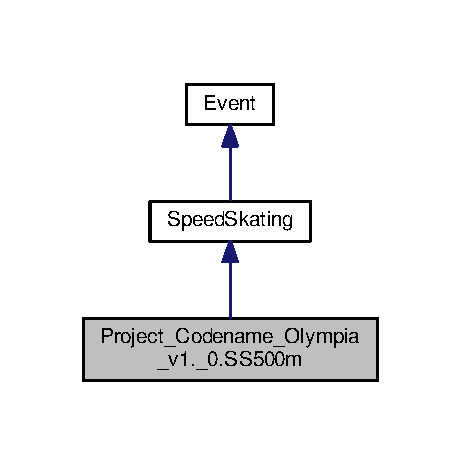
\includegraphics[width=221pt]{classProject__Codename__Olympia__v1_1_1__0_1_1SS500m__inherit__graph}
\end{center}
\end{figure}


Collaboration diagram for Project\+\_\+\+Codename\+\_\+\+Olympia\+\_\+v1.\+\_\+0.\+S\+S500m\+:
\nopagebreak
\begin{figure}[H]
\begin{center}
\leavevmode
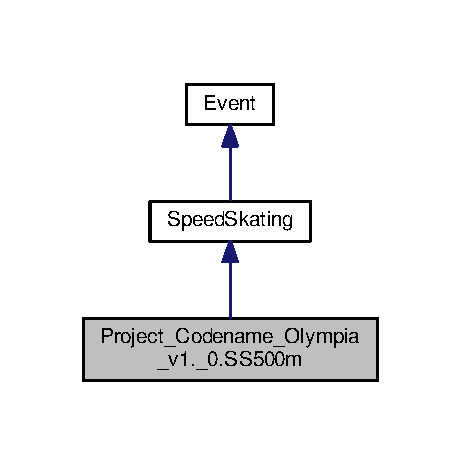
\includegraphics[width=221pt]{classProject__Codename__Olympia__v1_1_1__0_1_1SS500m__coll__graph}
\end{center}
\end{figure}
\subsection*{Public Member Functions}
\begin{DoxyCompactItemize}
\item 
\hyperlink{classProject__Codename__Olympia__v1_1_1__0_1_1SS500m_af01c484ae40be1166c5bc473b8876002}{S\+S500m} ()
\item 
override double \hyperlink{classProject__Codename__Olympia__v1_1_1__0_1_1SS500m_a1fc1ed5e2b6d1fa4d1921a3d155c6a6f}{ss\+Time} ()
\item 
override int \hyperlink{classProject__Codename__Olympia__v1_1_1__0_1_1SS500m_a7b5584a50c59e67457f86ebd38b8e4a8}{event\+Num} ()
\item 
override void \hyperlink{classProject__Codename__Olympia__v1_1_1__0_1_1SS500m_a28582161ab61bb80635656e48ebfc664}{run\+Event} (List$<$ \hyperlink{classProject__Codename__Olympia__v1_1_1__0_1_1Judge}{Judge} $>$ j, List$<$ \hyperlink{classProject__Codename__Olympia__v1_1_1__0_1_1Team}{Team} $>$ t)
\item 
override void \hyperlink{classProject__Codename__Olympia__v1_1_1__0_1_1SS500m_a11d698b484f98493d11661d43fa3ec12}{sched\+Event} (List$<$ \hyperlink{classProject__Codename__Olympia__v1_1_1__0_1_1Judge}{Judge} $>$ j, List$<$ \hyperlink{classProject__Codename__Olympia__v1_1_1__0_1_1Team}{Team} $>$ t)
\end{DoxyCompactItemize}


\subsection{Detailed Description}
\hyperlink{classProject__Codename__Olympia__v1_1_1__0_1_1SS500m}{S\+S500m} is one of the 3 \hyperlink{classProject__Codename__Olympia__v1_1_1__0_1_1SpeedSkating}{Speed\+Skating} events. 

D\+E\+F\+I\+N\+I\+T\+I\+ON\+: Form of speed skating where athletes utilize inline skates and race around a 400m rink 1.\+25 times. Whichever athlete crosses the finish line first has the lowest time.

C\+O\+N\+S\+T\+R\+A\+I\+N\+TS\+: A maximum of four athletes compete at a given time.\begin{DoxyAuthor}{Author}
Landen Marchand 
\end{DoxyAuthor}


\subsection{Constructor \& Destructor Documentation}
\mbox{\Hypertarget{classProject__Codename__Olympia__v1_1_1__0_1_1SS500m_af01c484ae40be1166c5bc473b8876002}\label{classProject__Codename__Olympia__v1_1_1__0_1_1SS500m_af01c484ae40be1166c5bc473b8876002}} 
\index{Project\+\_\+\+Codename\+\_\+\+Olympia\+\_\+v1\+::\+\_\+0\+::\+S\+S500m@{Project\+\_\+\+Codename\+\_\+\+Olympia\+\_\+v1\+::\+\_\+0\+::\+S\+S500m}!S\+S500m@{S\+S500m}}
\index{S\+S500m@{S\+S500m}!Project\+\_\+\+Codename\+\_\+\+Olympia\+\_\+v1\+::\+\_\+0\+::\+S\+S500m@{Project\+\_\+\+Codename\+\_\+\+Olympia\+\_\+v1\+::\+\_\+0\+::\+S\+S500m}}
\subsubsection{\texorpdfstring{S\+S500m()}{SS500m()}}
{\footnotesize\ttfamily Project\+\_\+\+Codename\+\_\+\+Olympia\+\_\+v1.\+\_\+0.\+S\+S500m.\+S\+S500m (\begin{DoxyParamCaption}{ }\end{DoxyParamCaption})\hspace{0.3cm}{\ttfamily [inline]}}

Default Constructor Provided Automatically 
\begin{DoxyParams}{Parameters}
{\em None} & \\
\hline
\end{DoxyParams}
\begin{DoxyReturn}{Returns}
Default Values 
\end{DoxyReturn}


\subsection{Member Function Documentation}
\mbox{\Hypertarget{classProject__Codename__Olympia__v1_1_1__0_1_1SS500m_a7b5584a50c59e67457f86ebd38b8e4a8}\label{classProject__Codename__Olympia__v1_1_1__0_1_1SS500m_a7b5584a50c59e67457f86ebd38b8e4a8}} 
\index{Project\+\_\+\+Codename\+\_\+\+Olympia\+\_\+v1\+::\+\_\+0\+::\+S\+S500m@{Project\+\_\+\+Codename\+\_\+\+Olympia\+\_\+v1\+::\+\_\+0\+::\+S\+S500m}!event\+Num@{event\+Num}}
\index{event\+Num@{event\+Num}!Project\+\_\+\+Codename\+\_\+\+Olympia\+\_\+v1\+::\+\_\+0\+::\+S\+S500m@{Project\+\_\+\+Codename\+\_\+\+Olympia\+\_\+v1\+::\+\_\+0\+::\+S\+S500m}}
\subsubsection{\texorpdfstring{event\+Num()}{eventNum()}}
{\footnotesize\ttfamily override int Project\+\_\+\+Codename\+\_\+\+Olympia\+\_\+v1.\+\_\+0.\+S\+S500m.\+event\+Num (\begin{DoxyParamCaption}{ }\end{DoxyParamCaption})\hspace{0.3cm}{\ttfamily [inline]}, {\ttfamily [virtual]}}

Function to override inherited \hyperlink{classProject__Codename__Olympia__v1_1_1__0_1_1SS500m_a7b5584a50c59e67457f86ebd38b8e4a8}{event\+Num()} function 

Implements \hyperlink{classProject__Codename__Olympia__v1_1_1__0_1_1Event_ad1154ef4dd1dec29d8ebf5614d84b1f3}{Project\+\_\+\+Codename\+\_\+\+Olympia\+\_\+v1.\+\_\+0.\+Event}.

\mbox{\Hypertarget{classProject__Codename__Olympia__v1_1_1__0_1_1SS500m_a28582161ab61bb80635656e48ebfc664}\label{classProject__Codename__Olympia__v1_1_1__0_1_1SS500m_a28582161ab61bb80635656e48ebfc664}} 
\index{Project\+\_\+\+Codename\+\_\+\+Olympia\+\_\+v1\+::\+\_\+0\+::\+S\+S500m@{Project\+\_\+\+Codename\+\_\+\+Olympia\+\_\+v1\+::\+\_\+0\+::\+S\+S500m}!run\+Event@{run\+Event}}
\index{run\+Event@{run\+Event}!Project\+\_\+\+Codename\+\_\+\+Olympia\+\_\+v1\+::\+\_\+0\+::\+S\+S500m@{Project\+\_\+\+Codename\+\_\+\+Olympia\+\_\+v1\+::\+\_\+0\+::\+S\+S500m}}
\subsubsection{\texorpdfstring{run\+Event()}{runEvent()}}
{\footnotesize\ttfamily override void Project\+\_\+\+Codename\+\_\+\+Olympia\+\_\+v1.\+\_\+0.\+S\+S500m.\+run\+Event (\begin{DoxyParamCaption}\item[{List$<$ \hyperlink{classProject__Codename__Olympia__v1_1_1__0_1_1Judge}{Judge} $>$}]{j,  }\item[{List$<$ \hyperlink{classProject__Codename__Olympia__v1_1_1__0_1_1Team}{Team} $>$}]{t }\end{DoxyParamCaption})\hspace{0.3cm}{\ttfamily [inline]}, {\ttfamily [virtual]}}

Function to override inherited run\+Event(..) function 

Implements \hyperlink{classProject__Codename__Olympia__v1_1_1__0_1_1Event_ac6ff060da23153c02da49937dcf9f326}{Project\+\_\+\+Codename\+\_\+\+Olympia\+\_\+v1.\+\_\+0.\+Event}.

\mbox{\Hypertarget{classProject__Codename__Olympia__v1_1_1__0_1_1SS500m_a11d698b484f98493d11661d43fa3ec12}\label{classProject__Codename__Olympia__v1_1_1__0_1_1SS500m_a11d698b484f98493d11661d43fa3ec12}} 
\index{Project\+\_\+\+Codename\+\_\+\+Olympia\+\_\+v1\+::\+\_\+0\+::\+S\+S500m@{Project\+\_\+\+Codename\+\_\+\+Olympia\+\_\+v1\+::\+\_\+0\+::\+S\+S500m}!sched\+Event@{sched\+Event}}
\index{sched\+Event@{sched\+Event}!Project\+\_\+\+Codename\+\_\+\+Olympia\+\_\+v1\+::\+\_\+0\+::\+S\+S500m@{Project\+\_\+\+Codename\+\_\+\+Olympia\+\_\+v1\+::\+\_\+0\+::\+S\+S500m}}
\subsubsection{\texorpdfstring{sched\+Event()}{schedEvent()}}
{\footnotesize\ttfamily override void Project\+\_\+\+Codename\+\_\+\+Olympia\+\_\+v1.\+\_\+0.\+S\+S500m.\+sched\+Event (\begin{DoxyParamCaption}\item[{List$<$ \hyperlink{classProject__Codename__Olympia__v1_1_1__0_1_1Judge}{Judge} $>$}]{j,  }\item[{List$<$ \hyperlink{classProject__Codename__Olympia__v1_1_1__0_1_1Team}{Team} $>$}]{t }\end{DoxyParamCaption})\hspace{0.3cm}{\ttfamily [inline]}, {\ttfamily [virtual]}}

Function to override inherited sched\+Event(..) function 

Implements \hyperlink{classProject__Codename__Olympia__v1_1_1__0_1_1Event_abb4e2b9c28527b9a28395f2fe9192196}{Project\+\_\+\+Codename\+\_\+\+Olympia\+\_\+v1.\+\_\+0.\+Event}.

\mbox{\Hypertarget{classProject__Codename__Olympia__v1_1_1__0_1_1SS500m_a1fc1ed5e2b6d1fa4d1921a3d155c6a6f}\label{classProject__Codename__Olympia__v1_1_1__0_1_1SS500m_a1fc1ed5e2b6d1fa4d1921a3d155c6a6f}} 
\index{Project\+\_\+\+Codename\+\_\+\+Olympia\+\_\+v1\+::\+\_\+0\+::\+S\+S500m@{Project\+\_\+\+Codename\+\_\+\+Olympia\+\_\+v1\+::\+\_\+0\+::\+S\+S500m}!ss\+Time@{ss\+Time}}
\index{ss\+Time@{ss\+Time}!Project\+\_\+\+Codename\+\_\+\+Olympia\+\_\+v1\+::\+\_\+0\+::\+S\+S500m@{Project\+\_\+\+Codename\+\_\+\+Olympia\+\_\+v1\+::\+\_\+0\+::\+S\+S500m}}
\subsubsection{\texorpdfstring{ss\+Time()}{ssTime()}}
{\footnotesize\ttfamily override double Project\+\_\+\+Codename\+\_\+\+Olympia\+\_\+v1.\+\_\+0.\+S\+S500m.\+ss\+Time (\begin{DoxyParamCaption}{ }\end{DoxyParamCaption})\hspace{0.3cm}{\ttfamily [inline]}, {\ttfamily [virtual]}}

Function to override inherited \hyperlink{classProject__Codename__Olympia__v1_1_1__0_1_1SS500m_a1fc1ed5e2b6d1fa4d1921a3d155c6a6f}{ss\+Time()} function 

Implements \hyperlink{classProject__Codename__Olympia__v1_1_1__0_1_1SpeedSkating_acedc7b2f1bfab95ee054531364ea50fb}{Project\+\_\+\+Codename\+\_\+\+Olympia\+\_\+v1.\+\_\+0.\+Speed\+Skating}.



The documentation for this class was generated from the following file\+:\begin{DoxyCompactItemize}
\item 
Class1.\+cs\end{DoxyCompactItemize}

\hypertarget{interfaceProject__Codename__Olympia__v1_1_1__0_1_1SpeedSkating_1_1ssInheritance}{}\section{Project\+\_\+\+Codename\+\_\+\+Olympia\+\_\+v1.\+\_\+0.\+Speed\+Skating.\+ss\+Inheritance Interface Reference}
\label{interfaceProject__Codename__Olympia__v1_1_1__0_1_1SpeedSkating_1_1ssInheritance}\index{Project\+\_\+\+Codename\+\_\+\+Olympia\+\_\+v1.\+\_\+0.\+Speed\+Skating.\+ss\+Inheritance@{Project\+\_\+\+Codename\+\_\+\+Olympia\+\_\+v1.\+\_\+0.\+Speed\+Skating.\+ss\+Inheritance}}
\subsection*{Public Member Functions}
\begin{DoxyCompactItemize}
\item 
\mbox{\Hypertarget{interfaceProject__Codename__Olympia__v1_1_1__0_1_1SpeedSkating_1_1ssInheritance_a209a8c48215583ce3c04f5f19f75325e}\label{interfaceProject__Codename__Olympia__v1_1_1__0_1_1SpeedSkating_1_1ssInheritance_a209a8c48215583ce3c04f5f19f75325e}} 
double {\bfseries ss\+Time} ()
\end{DoxyCompactItemize}


\subsection{Detailed Description}
Inheritance member function for \hyperlink{classProject__Codename__Olympia__v1_1_1__0_1_1SpeedSkating}{Speed\+Skating} events 
\begin{DoxyParams}{Parameters}
{\em none} & \\
\hline
\end{DoxyParams}
\begin{DoxyReturn}{Returns}
int pertaining to event ID 
\end{DoxyReturn}


The documentation for this interface was generated from the following file\+:\begin{DoxyCompactItemize}
\item 
Class1.\+cs\end{DoxyCompactItemize}

\hypertarget{interfaceProject__Codename__Olympia__v1_1_1__0_1_1FigureSkating_1_1ssInheritance}{}\section{Project\+\_\+\+Codename\+\_\+\+Olympia\+\_\+v1.\+\_\+0.\+Figure\+Skating.\+ss\+Inheritance Interface Reference}
\label{interfaceProject__Codename__Olympia__v1_1_1__0_1_1FigureSkating_1_1ssInheritance}\index{Project\+\_\+\+Codename\+\_\+\+Olympia\+\_\+v1.\+\_\+0.\+Figure\+Skating.\+ss\+Inheritance@{Project\+\_\+\+Codename\+\_\+\+Olympia\+\_\+v1.\+\_\+0.\+Figure\+Skating.\+ss\+Inheritance}}
\subsection*{Public Member Functions}
\begin{DoxyCompactItemize}
\item 
\mbox{\Hypertarget{interfaceProject__Codename__Olympia__v1_1_1__0_1_1FigureSkating_1_1ssInheritance_a746d4c0a4f9e66c645a2764a4df90451}\label{interfaceProject__Codename__Olympia__v1_1_1__0_1_1FigureSkating_1_1ssInheritance_a746d4c0a4f9e66c645a2764a4df90451}} 
double {\bfseries fs\+Score} ()
\end{DoxyCompactItemize}


\subsection{Detailed Description}
Interface so \hyperlink{classProject__Codename__Olympia__v1_1_1__0_1_1FigureSkating}{Figure\+Skating} events can utilize inherited functions 

The documentation for this interface was generated from the following file\+:\begin{DoxyCompactItemize}
\item 
Class1.\+cs\end{DoxyCompactItemize}

\hypertarget{classProject__Codename__Olympia__v1_1_1__0_1_1Team}{}\section{Project\+\_\+\+Codename\+\_\+\+Olympia\+\_\+v1.\+\_\+0.\+Team Class Reference}
\label{classProject__Codename__Olympia__v1_1_1__0_1_1Team}\index{Project\+\_\+\+Codename\+\_\+\+Olympia\+\_\+v1.\+\_\+0.\+Team@{Project\+\_\+\+Codename\+\_\+\+Olympia\+\_\+v1.\+\_\+0.\+Team}}


\hyperlink{classProject__Codename__Olympia__v1_1_1__0_1_1Team}{Team} class to house the team name.  


\subsection*{Public Member Functions}
\begin{DoxyCompactItemize}
\item 
\hyperlink{classProject__Codename__Olympia__v1_1_1__0_1_1Team_a370f46a59abab44451339138a0bf56aa}{Team} ()
\item 
int \hyperlink{classProject__Codename__Olympia__v1_1_1__0_1_1Team_a952816965dd529a15593315d18e38afc}{team\+Size} ()
\item 
void \hyperlink{classProject__Codename__Olympia__v1_1_1__0_1_1Team_a2f6a8ccddb47c40e497252321bcda811}{add\+Athlete} ()
\item 
void \hyperlink{classProject__Codename__Olympia__v1_1_1__0_1_1Team_ad172848f51c93bc1dcd0edc4e478ab23}{delete\+Athlete} ()
\end{DoxyCompactItemize}
\subsection*{Properties}
\begin{DoxyCompactItemize}
\item 
string \hyperlink{classProject__Codename__Olympia__v1_1_1__0_1_1Team_ae9c37c693f3d3254986cbea43819c946}{country\+Name}\hspace{0.3cm}{\ttfamily  \mbox{[}get, set\mbox{]}}
\end{DoxyCompactItemize}


\subsection{Detailed Description}
\hyperlink{classProject__Codename__Olympia__v1_1_1__0_1_1Team}{Team} class to house the team name. 

D\+E\+F\+I\+N\+I\+T\+I\+ON\+: Represents each country in the Winter Olympics.

C\+O\+N\+S\+T\+R\+A\+I\+N\+TS\+: There must be the same amount of males as females in a team. There is to only be one country per team.\begin{DoxyAuthor}{Author}
Landen Marchand 
\end{DoxyAuthor}


\subsection{Constructor \& Destructor Documentation}
\mbox{\Hypertarget{classProject__Codename__Olympia__v1_1_1__0_1_1Team_a370f46a59abab44451339138a0bf56aa}\label{classProject__Codename__Olympia__v1_1_1__0_1_1Team_a370f46a59abab44451339138a0bf56aa}} 
\index{Project\+\_\+\+Codename\+\_\+\+Olympia\+\_\+v1\+::\+\_\+0\+::\+Team@{Project\+\_\+\+Codename\+\_\+\+Olympia\+\_\+v1\+::\+\_\+0\+::\+Team}!Team@{Team}}
\index{Team@{Team}!Project\+\_\+\+Codename\+\_\+\+Olympia\+\_\+v1\+::\+\_\+0\+::\+Team@{Project\+\_\+\+Codename\+\_\+\+Olympia\+\_\+v1\+::\+\_\+0\+::\+Team}}
\subsubsection{\texorpdfstring{Team()}{Team()}}
{\footnotesize\ttfamily Project\+\_\+\+Codename\+\_\+\+Olympia\+\_\+v1.\+\_\+0.\+Team.\+Team (\begin{DoxyParamCaption}{ }\end{DoxyParamCaption})\hspace{0.3cm}{\ttfamily [inline]}}

Default Constructor Provided Automatically 
\begin{DoxyParams}{Parameters}
{\em None} & \\
\hline
\end{DoxyParams}
\begin{DoxyReturn}{Returns}
Default Values 
\end{DoxyReturn}


\subsection{Member Function Documentation}
\mbox{\Hypertarget{classProject__Codename__Olympia__v1_1_1__0_1_1Team_a2f6a8ccddb47c40e497252321bcda811}\label{classProject__Codename__Olympia__v1_1_1__0_1_1Team_a2f6a8ccddb47c40e497252321bcda811}} 
\index{Project\+\_\+\+Codename\+\_\+\+Olympia\+\_\+v1\+::\+\_\+0\+::\+Team@{Project\+\_\+\+Codename\+\_\+\+Olympia\+\_\+v1\+::\+\_\+0\+::\+Team}!add\+Athlete@{add\+Athlete}}
\index{add\+Athlete@{add\+Athlete}!Project\+\_\+\+Codename\+\_\+\+Olympia\+\_\+v1\+::\+\_\+0\+::\+Team@{Project\+\_\+\+Codename\+\_\+\+Olympia\+\_\+v1\+::\+\_\+0\+::\+Team}}
\subsubsection{\texorpdfstring{add\+Athlete()}{addAthlete()}}
{\footnotesize\ttfamily void Project\+\_\+\+Codename\+\_\+\+Olympia\+\_\+v1.\+\_\+0.\+Team.\+add\+Athlete (\begin{DoxyParamCaption}{ }\end{DoxyParamCaption})\hspace{0.3cm}{\ttfamily [inline]}}

Adds an athlete to a respective team 
\begin{DoxyParams}{Parameters}
{\em none} & \\
\hline
\end{DoxyParams}
\begin{DoxyReturn}{Returns}
none 
\end{DoxyReturn}
\mbox{\Hypertarget{classProject__Codename__Olympia__v1_1_1__0_1_1Team_ad172848f51c93bc1dcd0edc4e478ab23}\label{classProject__Codename__Olympia__v1_1_1__0_1_1Team_ad172848f51c93bc1dcd0edc4e478ab23}} 
\index{Project\+\_\+\+Codename\+\_\+\+Olympia\+\_\+v1\+::\+\_\+0\+::\+Team@{Project\+\_\+\+Codename\+\_\+\+Olympia\+\_\+v1\+::\+\_\+0\+::\+Team}!delete\+Athlete@{delete\+Athlete}}
\index{delete\+Athlete@{delete\+Athlete}!Project\+\_\+\+Codename\+\_\+\+Olympia\+\_\+v1\+::\+\_\+0\+::\+Team@{Project\+\_\+\+Codename\+\_\+\+Olympia\+\_\+v1\+::\+\_\+0\+::\+Team}}
\subsubsection{\texorpdfstring{delete\+Athlete()}{deleteAthlete()}}
{\footnotesize\ttfamily void Project\+\_\+\+Codename\+\_\+\+Olympia\+\_\+v1.\+\_\+0.\+Team.\+delete\+Athlete (\begin{DoxyParamCaption}{ }\end{DoxyParamCaption})\hspace{0.3cm}{\ttfamily [inline]}}

Deletes an athlete from a respective team 
\begin{DoxyParams}{Parameters}
{\em none} & \\
\hline
\end{DoxyParams}
\begin{DoxyReturn}{Returns}
none 
\end{DoxyReturn}
\mbox{\Hypertarget{classProject__Codename__Olympia__v1_1_1__0_1_1Team_a952816965dd529a15593315d18e38afc}\label{classProject__Codename__Olympia__v1_1_1__0_1_1Team_a952816965dd529a15593315d18e38afc}} 
\index{Project\+\_\+\+Codename\+\_\+\+Olympia\+\_\+v1\+::\+\_\+0\+::\+Team@{Project\+\_\+\+Codename\+\_\+\+Olympia\+\_\+v1\+::\+\_\+0\+::\+Team}!team\+Size@{team\+Size}}
\index{team\+Size@{team\+Size}!Project\+\_\+\+Codename\+\_\+\+Olympia\+\_\+v1\+::\+\_\+0\+::\+Team@{Project\+\_\+\+Codename\+\_\+\+Olympia\+\_\+v1\+::\+\_\+0\+::\+Team}}
\subsubsection{\texorpdfstring{team\+Size()}{teamSize()}}
{\footnotesize\ttfamily int Project\+\_\+\+Codename\+\_\+\+Olympia\+\_\+v1.\+\_\+0.\+Team.\+team\+Size (\begin{DoxyParamCaption}{ }\end{DoxyParamCaption})\hspace{0.3cm}{\ttfamily [inline]}}

Function to return current number of athletes in a specific team 
\begin{DoxyParams}{Parameters}
{\em none} & \\
\hline
\end{DoxyParams}
\begin{DoxyReturn}{Returns}
int for number of athletes on the team 
\end{DoxyReturn}


\subsection{Property Documentation}
\mbox{\Hypertarget{classProject__Codename__Olympia__v1_1_1__0_1_1Team_ae9c37c693f3d3254986cbea43819c946}\label{classProject__Codename__Olympia__v1_1_1__0_1_1Team_ae9c37c693f3d3254986cbea43819c946}} 
\index{Project\+\_\+\+Codename\+\_\+\+Olympia\+\_\+v1\+::\+\_\+0\+::\+Team@{Project\+\_\+\+Codename\+\_\+\+Olympia\+\_\+v1\+::\+\_\+0\+::\+Team}!country\+Name@{country\+Name}}
\index{country\+Name@{country\+Name}!Project\+\_\+\+Codename\+\_\+\+Olympia\+\_\+v1\+::\+\_\+0\+::\+Team@{Project\+\_\+\+Codename\+\_\+\+Olympia\+\_\+v1\+::\+\_\+0\+::\+Team}}
\subsubsection{\texorpdfstring{country\+Name}{countryName}}
{\footnotesize\ttfamily string Project\+\_\+\+Codename\+\_\+\+Olympia\+\_\+v1.\+\_\+0.\+Team.\+country\+Name\hspace{0.3cm}{\ttfamily [get]}, {\ttfamily [set]}}

Sets and gets team\textquotesingle{}s name, which is their country\textquotesingle{}s name 
\begin{DoxyParams}{Parameters}
{\em string} & for team name \\
\hline
\end{DoxyParams}
\begin{DoxyReturn}{Returns}
string of team name 
\end{DoxyReturn}


The documentation for this class was generated from the following file\+:\begin{DoxyCompactItemize}
\item 
Class1.\+cs\end{DoxyCompactItemize}

\hypertarget{classProject__Codename__Olympia__v1_1_1__0_1_1TeamForm}{}\section{Project\+\_\+\+Codename\+\_\+\+Olympia\+\_\+v1.\+\_\+0.\+Team\+Form Class Reference}
\label{classProject__Codename__Olympia__v1_1_1__0_1_1TeamForm}\index{Project\+\_\+\+Codename\+\_\+\+Olympia\+\_\+v1.\+\_\+0.\+Team\+Form@{Project\+\_\+\+Codename\+\_\+\+Olympia\+\_\+v1.\+\_\+0.\+Team\+Form}}


Inheritance diagram for Project\+\_\+\+Codename\+\_\+\+Olympia\+\_\+v1.\+\_\+0.\+Team\+Form\+:
\nopagebreak
\begin{figure}[H]
\begin{center}
\leavevmode
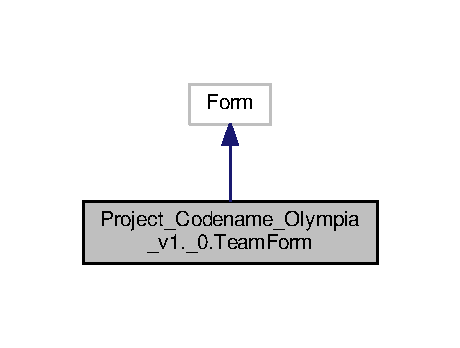
\includegraphics[width=221pt]{classProject__Codename__Olympia__v1_1_1__0_1_1TeamForm__inherit__graph}
\end{center}
\end{figure}


Collaboration diagram for Project\+\_\+\+Codename\+\_\+\+Olympia\+\_\+v1.\+\_\+0.\+Team\+Form\+:
\nopagebreak
\begin{figure}[H]
\begin{center}
\leavevmode
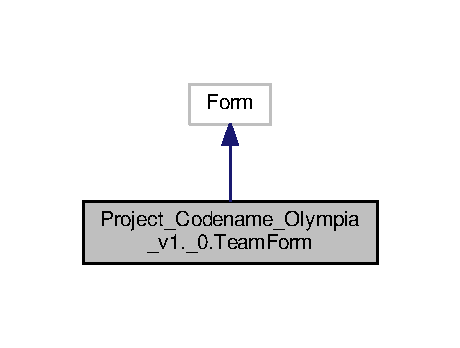
\includegraphics[width=221pt]{classProject__Codename__Olympia__v1_1_1__0_1_1TeamForm__coll__graph}
\end{center}
\end{figure}
\subsection*{Protected Member Functions}
\begin{DoxyCompactItemize}
\item 
override void \hyperlink{classProject__Codename__Olympia__v1_1_1__0_1_1TeamForm_a7896ce3551a76d8161138e412e507a17}{Dispose} (bool disposing)
\begin{DoxyCompactList}\small\item\em Clean up any resources being used. \end{DoxyCompactList}\end{DoxyCompactItemize}


\subsection{Member Function Documentation}
\mbox{\Hypertarget{classProject__Codename__Olympia__v1_1_1__0_1_1TeamForm_a7896ce3551a76d8161138e412e507a17}\label{classProject__Codename__Olympia__v1_1_1__0_1_1TeamForm_a7896ce3551a76d8161138e412e507a17}} 
\index{Project\+\_\+\+Codename\+\_\+\+Olympia\+\_\+v1\+::\+\_\+0\+::\+Team\+Form@{Project\+\_\+\+Codename\+\_\+\+Olympia\+\_\+v1\+::\+\_\+0\+::\+Team\+Form}!Dispose@{Dispose}}
\index{Dispose@{Dispose}!Project\+\_\+\+Codename\+\_\+\+Olympia\+\_\+v1\+::\+\_\+0\+::\+Team\+Form@{Project\+\_\+\+Codename\+\_\+\+Olympia\+\_\+v1\+::\+\_\+0\+::\+Team\+Form}}
\subsubsection{\texorpdfstring{Dispose()}{Dispose()}}
{\footnotesize\ttfamily override void Project\+\_\+\+Codename\+\_\+\+Olympia\+\_\+v1.\+\_\+0.\+Team\+Form.\+Dispose (\begin{DoxyParamCaption}\item[{bool}]{disposing }\end{DoxyParamCaption})\hspace{0.3cm}{\ttfamily [inline]}, {\ttfamily [protected]}}



Clean up any resources being used. 


\begin{DoxyParams}{Parameters}
{\em disposing} & true if managed resources should be disposed; otherwise, false.\\
\hline
\end{DoxyParams}


The documentation for this class was generated from the following files\+:\begin{DoxyCompactItemize}
\item 
Form2.\+cs\item 
Form2.\+Designer.\+cs\end{DoxyCompactItemize}

%--- End generated contents ---

% Index
\backmatter
\newpage
\phantomsection
\clearemptydoublepage
\addcontentsline{toc}{chapter}{Index}
\printindex

\end{document}
